\documentclass[a4paper,12pt,twoside]{includes/ThesisStyle}

\usepackage[T1]{fontenc} %%%key to get copy and paste for the code!
%\usepackage[utf8]{inputenc} %%% to support copy and paste with accents for frnehc stuff
\usepackage{times}
\usepackage{ifthen}
\usepackage{xspace}
\usepackage{alltt}
\usepackage{latexsym}
\usepackage{url}            
\usepackage{amssymb}
\usepackage{amsfonts}
\usepackage{amsmath}
\usepackage{stmaryrd}
\usepackage{enumerate}
\usepackage{cite}
%\usepackage[pdftex,colorlinks=true,pdfstartview=FitV,linkcolor=blue,citecolor=blue,urlcolor=blue]{hyperref}
\usepackage{xspace}
%\usepackage{graphicx}
\usepackage{subfigure}
\usepackage[scaled=0.85]{helvet}
        
        
\newcommand{\sepe}{\mbox{>>}}
\newcommand{\pack}[1]{\emph{#1}}
\newcommand{\ozo}{\textsc{oZone}\xspace}
\newcommand\currentissues{\par\smallskip\textbf{Current Issues -- }}

\newboolean{showcomments}
\setboolean{showcomments}{true}
\ifthenelse{\boolean{showcomments}}
  {\newcommand{\bnote}[2]{
	\fbox{\bfseries\sffamily\scriptsize#1}
    {\sf\small$\blacktriangleright$\textit{#2}$\blacktriangleleft$}
    % \marginpar{\fbox{\bfseries\sffamily#1}}
   }
   \newcommand{\cvsversion}{\emph{\scriptsize$-$Id: macros.tex,v 1.1.1.1 2007/02/28 13:43:36 bergel Exp $-$}}
  }
  {\newcommand{\bnote}[2]{}
   \newcommand{\cvsversion}{}
  } 


\newcommand{\here}{\bnote{***}{CONTINUE HERE}}
\newcommand{\nb}[1]{\bnote{NB}{#1}}
\newcommand{\fix}[1]{\bnote{FIX}{#1}}
%%%% add your own macros 

\newcommand{\sd}[1]{\bnote{Stef}{#1}}
\newcommand{\ja}[1]{\bnote{Jannik}{#1}}
\newcommand{\na}[1]{\bnote{Nico}{#1}}
%%% 


\newcommand{\figref}[1]{Figure~\ref{fig:#1}}
\newcommand{\figlabel}[1]{\label{fig:#1}}
\newcommand{\tabref}[1]{Table~\ref{tab:#1}}
\newcommand{\layout}[1]{#1}
\newcommand{\commented}[1]{}
\newcommand{\secref}[1]{Section \ref{sec:#1}}
\newcommand{\seclabel}[1]{\label{sec:#1}}

%\newcommand{\ct}[1]{\textsf{#1}}
\newcommand{\stCode}[1]{\textsf{#1}}
\newcommand{\stMethod}[1]{\textsf{#1}}
\newcommand{\sep}{\texttt{>>}\xspace}
\newcommand{\stAssoc}{\texttt{->}\xspace}

\newcommand{\stBar}{$\mid$}
\newcommand{\stSelector}{$\gg$}
\newcommand{\ret}{\^{}}
\newcommand{\msup}{$>$}
%\newcommand{\ret}{$\uparrow$\xspace}

\newcommand{\myparagraph}[1]{\noindent\textbf{#1.}}
\newcommand{\eg}{\emph{e.g.,}\xspace}
\newcommand{\ie}{\emph{i.e.,}\xspace}
\newcommand{\ct}[1]{{\textsf{#1}}\xspace}


\newenvironment{code}
    {\begin{alltt}\sffamily}
    {\end{alltt}\normalsize}

\newcommand{\defaultScale}{0.55}
\newcommand{\pic}[3]{
   \begin{figure}[h]
   \begin{center}
   \includegraphics[scale=\defaultScale]{#1}
   \caption{#2}
   \label{#3}
   \end{center}
   \end{figure}
}

\newcommand{\twocolumnpic}[3]{
   \begin{figure*}[!ht]
   \begin{center}
   \includegraphics[scale=\defaultScale]{#1}
   \caption{#2}
   \label{#3}
   \end{center}
   \end{figure*}}

\newcommand{\infe}{$<$}
\newcommand{\supe}{$\rightarrow$\xspace}
\newcommand{\di}{$\gg$\xspace}
\newcommand{\adhoc}{\textit{ad-hoc}\xspace}

\usepackage{url}            
\makeatletter
\def\url@leostyle{%
  \@ifundefined{selectfont}{\def\UrlFont{\sf}}{\def\UrlFont{\small\sffamily}}}
\makeatother
% Now actually use the newly defined style.
\urlstyle{leo}



\usepackage{amsmath,amssymb}             % AMS Math
% \usepackage[french]{babel}
\usepackage[latin1]{inputenc}
\usepackage[T1]{fontenc}
\usepackage[left=1.5in,right=1.3in,top=1.1in,bottom=1.1in,includefoot,includehead,headheight=13.6pt]{geometry}
\renewcommand{\baselinestretch}{1.05}

\usepackage{multicol}

% Table of contents for each chapter

\usepackage[nottoc, notlof, notlot]{tocbibind}
\usepackage{minitoc}
\setcounter{minitocdepth}{1}
\mtcindent=15pt
% Use \minitoc where to put a table of contents

\usepackage{enumitem}

\usepackage{aecompl}

% Glossary / list of abbreviations

%\usepackage[intoc]{nomencl}
%\renewcommand{\nomname}{List of Abbreviations}
%
%\makenomenclature

% My pdf code

\usepackage[pdftex]{graphicx}
\usepackage[a4paper,pagebackref,hyperindex=true]{hyperref}

\usepackage{pgfplotstable,booktabs,colortbl}
\pgfplotsset{compat=1.8}

% Links in pdf
\usepackage{color}
\definecolor{linkcol}{rgb}{0,0,0.4} 
\definecolor{citecol}{rgb}{0.5,0,0} 

% Change this to change the informations included in the pdf file

% See hyperref documentation for information on those parameters

\hypersetup
{
bookmarksopen=true,
pdftitle="Sista: a Metacircular Architecture for Runtime Optimisation Persistence",
pdfauthor="Clement BERA", 
pdfsubject="Thesis", %subject of the document
%pdftoolbar=false, % toolbar hidden
pdfmenubar=true, %menubar shown
pdfhighlight=/O, %effect of clicking on a link
colorlinks=true, %couleurs sur les liens hypertextes
pdfpagemode=None, %aucun mode de page
pdfpagelayout=SinglePage, %ouverture en simple page
pdffitwindow=true, %pages ouvertes entierement dans toute la fenetre
linkcolor=linkcol, %couleur des liens hypertextes internes
citecolor=citecol, %couleur des liens pour les citations
urlcolor=linkcol %couleur des liens pour les url
}

% definitions.
% -------------------

\setcounter{secnumdepth}{3}
\setcounter{tocdepth}{1}

% Some useful commands and shortcut for maths:  partial derivative and stuff

\newcommand{\pd}[2]{\frac{\partial #1}{\partial #2}}
\def\abs{\operatorname{abs}}
\def\argmax{\operatornamewithlimits{arg\,max}}
\def\argmin{\operatornamewithlimits{arg\,min}}
\def\diag{\operatorname{Diag}}
\newcommand{\eqRef}[1]{(\ref{#1})}

\usepackage{rotating}                    % Sideways of figures & tables
%\usepackage{bibunits}
%\usepackage[sectionbib]{chapterbib}          % Cross-reference package (Natural BiB)
%\usepackage{natbib}                  % Put References at the end of each chapter
                                         % Do not put 'sectionbib' option here.
                                         % Sectionbib option in 'natbib' will do.
\usepackage{fancyhdr}                    % Fancy Header and Footer

% \usepackage{txfonts}                     % Public Times New Roman text & math font
  
%%% Fancy Header %%%%%%%%%%%%%%%%%%%%%%%%%%%%%%%%%%%%%%%%%%%%%%%%%%%%%%%%%%%%%%%%%%
% Fancy Header Style Options

\pagestyle{fancy}                       % Sets fancy header and footer
\fancyfoot{}                            % Delete current footer settings

%\renewcommand{\chaptermark}[1]{         % Lower Case Chapter marker style
%  \markboth{\chaptername\ \thechapter.\ #1}}{}} %

%\renewcommand{\sectionmark}[1]{         % Lower case Section marker style
%  \markright{\thesection.\ #1}}         %

\fancyhead[LE,RO]{\bfseries\thepage}    % Page number (boldface) in left on even
% pages and right on odd pages
\fancyhead[RE]{\bfseries\nouppercase{\leftmark}}      % Chapter in the right on even pages
\fancyhead[LO]{\bfseries\nouppercase{\rightmark}}     % Section in the left on odd pages

\let\headruleORIG\headrule
\renewcommand{\headrule}{\color{black} \headruleORIG}
\renewcommand{\headrulewidth}{1.0pt}
\usepackage{colortbl}
\arrayrulecolor{black}

\fancypagestyle{plain}{
  \fancyhead{}
  \fancyfoot{}
  \renewcommand{\headrulewidth}{0pt}
}

\usepackage{algorithm}
\usepackage[noend]{algorithmic}

%%% Clear Header %%%%%%%%%%%%%%%%%%%%%%%%%%%%%%%%%%%%%%%%%%%%%%%%%%%%%%%%%%%%%%%%%%
% Clear Header Style on the Last Empty Odd pages
\makeatletter

\def\cleardoublepage{\clearpage\if@twoside \ifodd\c@page\else%
  \hbox{}%
  \thispagestyle{empty}%              % Empty header styles
  \newpage%
  \if@twocolumn\hbox{}\newpage\fi\fi\fi}

\makeatother
 
%%%%%%%%%%%%%%%%%%%%%%%%%%%%%%%%%%%%%%%%%%%%%%%%%%%%%%%%%%%%%%%%%%%%%%%%%%%%%%% 
% Prints your review date and 'Draft Version' (From Josullvn, CS, CMU)
\newcommand{\reviewtimetoday}[2]{\special{!userdict begin
    /bop-hook{gsave 20 710 translate 45 rotate 0.8 setgray
      /Times-Roman findfont 12 scalefont setfont 0 0   moveto (#1) show
      0 -12 moveto (#2) show grestore}def end}}
% You can turn on or off this option.
% \reviewtimetoday{\today}{Draft Version}
%%%%%%%%%%%%%%%%%%%%%%%%%%%%%%%%%%%%%%%%%%%%%%%%%%%%%%%%%%%%%%%%%%%%%%%%%%%%%%% 

\newenvironment{maxime}[1]
{
\vspace*{0cm}
\hfill
\begin{minipage}{0.5\textwidth}%
%\rule[0.5ex]{\textwidth}{0.1mm}\\%
\hrulefill $\:$ {\bf #1}\\
%\vspace*{-0.25cm}
\it 
}%
{%

\hrulefill
\vspace*{0.5cm}%
\end{minipage}
}

\let\minitocORIG\minitoc
\renewcommand{\minitoc}{\minitocORIG \vspace{1.5em}}

\usepackage{multirow}
\usepackage{slashbox}

\newenvironment{bulletList}%
{ \begin{list}%
	{$\bullet$}%
	{\setlength{\labelwidth}{25pt}%
	 \setlength{\leftmargin}{30pt}%
	 \setlength{\itemsep}{\parsep}}}%
{ \end{list} }

\newtheorem{definition}{D�finition}
\renewcommand{\epsilon}{\varepsilon}

% centered page environment

\newenvironment{vcenterpage}
{\newpage\vspace*{\fill}\thispagestyle{empty}\renewcommand{\headrulewidth}{0pt}}
{\vspace*{\fill}}



\graphicspath{{.}{figures/}}
\newcommand \logoInria{./includes/logos/Inria}
\newcommand \logoRegion{./includes/logos/Region}
\newcommand \logoLifl{./includes/logos/lifl}
\newcommand \logoUSTL{./includes/logos/Lille1}

\let\wholebook=\relax

\begin{document}
\include{chapters/titlePage}
\dominitoc

\pagenumbering{roman}

\cleardoublepage

\section*{Acknowledgments}

I would like to thank my thesis supervisors St\'ephane Ducasse and Marcus Denker for allowing me to do a Ph.D at the RMoD group, as well as helping and supporting me during the three years of my Ph.D.

I thank the thesis reviewers and jury members Ga\"el Thomas, Laurence Tratt for kindly reviewing my thesis and providing me valuable feedback. I thank Laurence Duchien for leading the jury.

I would like to express my gratitude to Eliot Miranda for his first design of the Sista architecture and his support during the three years of my Ph.D. 

I would like to thank Tim Felgentreff for his evaluation of Sista architecture using the Squeak speed center.

For remarks on earlier versions of this thesis I thank (To confirm if they actually do it, potentially other people too) Guillermo Polito and Damien Cassou.

\cleardoublepage

\section*{Abstract}

Most high-level programming languages run on top of a virtual machine (VM) to abstract away from the underlying hardware. To reach high-performance, the VM typically relies on an optimising just-in-time compiler (JIT), which speculates on the program behavior based on its first runs to generate at runtime efficient machine code and speed-up the program execution. As multiple runs are required to speculate correctly on the program behavior, such a VM requires a certain amount of time at start-up to reach peak performance. The optimising JIT itself is usually compiled ahead-of-time to executable code as part of the VM.

The dissertation proposes an architecture for an optimising JIT, in which the optimised state of the VM can be persisted across multiple start-ups and the optimising JIT is running in the same runtime than the program executed. To do so, the optimising JIT is split in two parts. One part is high-level: it performs optimisations specific to the programming language run by the VM and is written in a metacircular style. Staying away from low-level details, this part can be read, edited and debugged while the program is running using the standard tool set of the programming language executed by the VM. The second part is low-level: it performs machine specific optimisations and is compiled ahead-of-time to executable code as part of the virtual machine. The two parts of the JIT use a well-defined intermediate representation to share the code to optimise. This representation is machine-independent and can be persisted across multiple start-ups, allowing the virtual machine to reach peak performance very quickly.

To validate the architecture, the dissertation includes the description of an implementation on top of Pharo Smalltalk and its virtual machine. The implementation is able to run a large set of benchmarks, from large application benchmarks provided by industrial users to micro-benchmarks used to measure the performance of specific code patterns. The optimising JIT is implemented according to the architecture proposed and shows significant speed-up (1.5x to 5x) over the current production virtual machine. In addition, large benchmarks show that peak performance can be reached almost immediately after start-up if the VM can reuse the optimised state persisted from another run.

\cleardoublepage

\section*{R\'esum\'e}

\tableofcontents
\listoffigures
%\listoftables

\mainmatter

\ifx\wholebook\relax\else

% --------------------------------------------
% Lulu:

    \documentclass[a4paper,12pt,twoside]{../includes/ThesisStyle}

	\usepackage[T1]{fontenc} %%%key to get copy and paste for the code!
%\usepackage[utf8]{inputenc} %%% to support copy and paste with accents for frnehc stuff
\usepackage{times}
\usepackage{ifthen}
\usepackage{xspace}
\usepackage{alltt}
\usepackage{latexsym}
\usepackage{url}            
\usepackage{amssymb}
\usepackage{amsfonts}
\usepackage{amsmath}
\usepackage{stmaryrd}
\usepackage{enumerate}
\usepackage{cite}
%\usepackage[pdftex,colorlinks=true,pdfstartview=FitV,linkcolor=blue,citecolor=blue,urlcolor=blue]{hyperref}
\usepackage{xspace}
%\usepackage{graphicx}
\usepackage{subfigure}
\usepackage[scaled=0.85]{helvet}
        
        
\newcommand{\sepe}{\mbox{>>}}
\newcommand{\pack}[1]{\emph{#1}}
\newcommand{\ozo}{\textsc{oZone}\xspace}
\newcommand\currentissues{\par\smallskip\textbf{Current Issues -- }}

\newboolean{showcomments}
\setboolean{showcomments}{true}
\ifthenelse{\boolean{showcomments}}
  {\newcommand{\bnote}[2]{
	\fbox{\bfseries\sffamily\scriptsize#1}
    {\sf\small$\blacktriangleright$\textit{#2}$\blacktriangleleft$}
    % \marginpar{\fbox{\bfseries\sffamily#1}}
   }
   \newcommand{\cvsversion}{\emph{\scriptsize$-$Id: macros.tex,v 1.1.1.1 2007/02/28 13:43:36 bergel Exp $-$}}
  }
  {\newcommand{\bnote}[2]{}
   \newcommand{\cvsversion}{}
  } 


\newcommand{\here}{\bnote{***}{CONTINUE HERE}}
\newcommand{\nb}[1]{\bnote{NB}{#1}}
\newcommand{\fix}[1]{\bnote{FIX}{#1}}
%%%% add your own macros 

\newcommand{\sd}[1]{\bnote{Stef}{#1}}
\newcommand{\ja}[1]{\bnote{Jannik}{#1}}
\newcommand{\na}[1]{\bnote{Nico}{#1}}
%%% 


\newcommand{\figref}[1]{Figure~\ref{fig:#1}}
\newcommand{\figlabel}[1]{\label{fig:#1}}
\newcommand{\tabref}[1]{Table~\ref{tab:#1}}
\newcommand{\layout}[1]{#1}
\newcommand{\commented}[1]{}
\newcommand{\secref}[1]{Section \ref{sec:#1}}
\newcommand{\seclabel}[1]{\label{sec:#1}}

%\newcommand{\ct}[1]{\textsf{#1}}
\newcommand{\stCode}[1]{\textsf{#1}}
\newcommand{\stMethod}[1]{\textsf{#1}}
\newcommand{\sep}{\texttt{>>}\xspace}
\newcommand{\stAssoc}{\texttt{->}\xspace}

\newcommand{\stBar}{$\mid$}
\newcommand{\stSelector}{$\gg$}
\newcommand{\ret}{\^{}}
\newcommand{\msup}{$>$}
%\newcommand{\ret}{$\uparrow$\xspace}

\newcommand{\myparagraph}[1]{\noindent\textbf{#1.}}
\newcommand{\eg}{\emph{e.g.,}\xspace}
\newcommand{\ie}{\emph{i.e.,}\xspace}
\newcommand{\ct}[1]{{\textsf{#1}}\xspace}


\newenvironment{code}
    {\begin{alltt}\sffamily}
    {\end{alltt}\normalsize}

\newcommand{\defaultScale}{0.55}
\newcommand{\pic}[3]{
   \begin{figure}[h]
   \begin{center}
   \includegraphics[scale=\defaultScale]{#1}
   \caption{#2}
   \label{#3}
   \end{center}
   \end{figure}
}

\newcommand{\twocolumnpic}[3]{
   \begin{figure*}[!ht]
   \begin{center}
   \includegraphics[scale=\defaultScale]{#1}
   \caption{#2}
   \label{#3}
   \end{center}
   \end{figure*}}

\newcommand{\infe}{$<$}
\newcommand{\supe}{$\rightarrow$\xspace}
\newcommand{\di}{$\gg$\xspace}
\newcommand{\adhoc}{\textit{ad-hoc}\xspace}

\usepackage{url}            
\makeatletter
\def\url@leostyle{%
  \@ifundefined{selectfont}{\def\UrlFont{\sf}}{\def\UrlFont{\small\sffamily}}}
\makeatother
% Now actually use the newly defined style.
\urlstyle{leo}



	\usepackage{amsmath,amssymb}             % AMS Math
% \usepackage[french]{babel}
\usepackage[latin1]{inputenc}
\usepackage[T1]{fontenc}
\usepackage[left=1.5in,right=1.3in,top=1.1in,bottom=1.1in,includefoot,includehead,headheight=13.6pt]{geometry}
\renewcommand{\baselinestretch}{1.05}

\usepackage{multicol}

% Table of contents for each chapter

\usepackage[nottoc, notlof, notlot]{tocbibind}
\usepackage{minitoc}
\setcounter{minitocdepth}{1}
\mtcindent=15pt
% Use \minitoc where to put a table of contents

\usepackage{enumitem}

\usepackage{aecompl}

% Glossary / list of abbreviations

%\usepackage[intoc]{nomencl}
%\renewcommand{\nomname}{List of Abbreviations}
%
%\makenomenclature

% My pdf code

\usepackage[pdftex]{graphicx}
\usepackage[a4paper,pagebackref,hyperindex=true]{hyperref}

\usepackage{pgfplotstable,booktabs,colortbl}
\pgfplotsset{compat=1.8}

% Links in pdf
\usepackage{color}
\definecolor{linkcol}{rgb}{0,0,0.4} 
\definecolor{citecol}{rgb}{0.5,0,0} 

% Change this to change the informations included in the pdf file

% See hyperref documentation for information on those parameters

\hypersetup
{
bookmarksopen=true,
pdftitle="Sista: a Metacircular Architecture for Runtime Optimisation Persistence",
pdfauthor="Clement BERA", 
pdfsubject="Thesis", %subject of the document
%pdftoolbar=false, % toolbar hidden
pdfmenubar=true, %menubar shown
pdfhighlight=/O, %effect of clicking on a link
colorlinks=true, %couleurs sur les liens hypertextes
pdfpagemode=None, %aucun mode de page
pdfpagelayout=SinglePage, %ouverture en simple page
pdffitwindow=true, %pages ouvertes entierement dans toute la fenetre
linkcolor=linkcol, %couleur des liens hypertextes internes
citecolor=citecol, %couleur des liens pour les citations
urlcolor=linkcol %couleur des liens pour les url
}

% definitions.
% -------------------

\setcounter{secnumdepth}{3}
\setcounter{tocdepth}{1}

% Some useful commands and shortcut for maths:  partial derivative and stuff

\newcommand{\pd}[2]{\frac{\partial #1}{\partial #2}}
\def\abs{\operatorname{abs}}
\def\argmax{\operatornamewithlimits{arg\,max}}
\def\argmin{\operatornamewithlimits{arg\,min}}
\def\diag{\operatorname{Diag}}
\newcommand{\eqRef}[1]{(\ref{#1})}

\usepackage{rotating}                    % Sideways of figures & tables
%\usepackage{bibunits}
%\usepackage[sectionbib]{chapterbib}          % Cross-reference package (Natural BiB)
%\usepackage{natbib}                  % Put References at the end of each chapter
                                         % Do not put 'sectionbib' option here.
                                         % Sectionbib option in 'natbib' will do.
\usepackage{fancyhdr}                    % Fancy Header and Footer

% \usepackage{txfonts}                     % Public Times New Roman text & math font
  
%%% Fancy Header %%%%%%%%%%%%%%%%%%%%%%%%%%%%%%%%%%%%%%%%%%%%%%%%%%%%%%%%%%%%%%%%%%
% Fancy Header Style Options

\pagestyle{fancy}                       % Sets fancy header and footer
\fancyfoot{}                            % Delete current footer settings

%\renewcommand{\chaptermark}[1]{         % Lower Case Chapter marker style
%  \markboth{\chaptername\ \thechapter.\ #1}}{}} %

%\renewcommand{\sectionmark}[1]{         % Lower case Section marker style
%  \markright{\thesection.\ #1}}         %

\fancyhead[LE,RO]{\bfseries\thepage}    % Page number (boldface) in left on even
% pages and right on odd pages
\fancyhead[RE]{\bfseries\nouppercase{\leftmark}}      % Chapter in the right on even pages
\fancyhead[LO]{\bfseries\nouppercase{\rightmark}}     % Section in the left on odd pages

\let\headruleORIG\headrule
\renewcommand{\headrule}{\color{black} \headruleORIG}
\renewcommand{\headrulewidth}{1.0pt}
\usepackage{colortbl}
\arrayrulecolor{black}

\fancypagestyle{plain}{
  \fancyhead{}
  \fancyfoot{}
  \renewcommand{\headrulewidth}{0pt}
}

\usepackage{algorithm}
\usepackage[noend]{algorithmic}

%%% Clear Header %%%%%%%%%%%%%%%%%%%%%%%%%%%%%%%%%%%%%%%%%%%%%%%%%%%%%%%%%%%%%%%%%%
% Clear Header Style on the Last Empty Odd pages
\makeatletter

\def\cleardoublepage{\clearpage\if@twoside \ifodd\c@page\else%
  \hbox{}%
  \thispagestyle{empty}%              % Empty header styles
  \newpage%
  \if@twocolumn\hbox{}\newpage\fi\fi\fi}

\makeatother
 
%%%%%%%%%%%%%%%%%%%%%%%%%%%%%%%%%%%%%%%%%%%%%%%%%%%%%%%%%%%%%%%%%%%%%%%%%%%%%%% 
% Prints your review date and 'Draft Version' (From Josullvn, CS, CMU)
\newcommand{\reviewtimetoday}[2]{\special{!userdict begin
    /bop-hook{gsave 20 710 translate 45 rotate 0.8 setgray
      /Times-Roman findfont 12 scalefont setfont 0 0   moveto (#1) show
      0 -12 moveto (#2) show grestore}def end}}
% You can turn on or off this option.
% \reviewtimetoday{\today}{Draft Version}
%%%%%%%%%%%%%%%%%%%%%%%%%%%%%%%%%%%%%%%%%%%%%%%%%%%%%%%%%%%%%%%%%%%%%%%%%%%%%%% 

\newenvironment{maxime}[1]
{
\vspace*{0cm}
\hfill
\begin{minipage}{0.5\textwidth}%
%\rule[0.5ex]{\textwidth}{0.1mm}\\%
\hrulefill $\:$ {\bf #1}\\
%\vspace*{-0.25cm}
\it 
}%
{%

\hrulefill
\vspace*{0.5cm}%
\end{minipage}
}

\let\minitocORIG\minitoc
\renewcommand{\minitoc}{\minitocORIG \vspace{1.5em}}

\usepackage{multirow}
\usepackage{slashbox}

\newenvironment{bulletList}%
{ \begin{list}%
	{$\bullet$}%
	{\setlength{\labelwidth}{25pt}%
	 \setlength{\leftmargin}{30pt}%
	 \setlength{\itemsep}{\parsep}}}%
{ \end{list} }

\newtheorem{definition}{D�finition}
\renewcommand{\epsilon}{\varepsilon}

% centered page environment

\newenvironment{vcenterpage}
{\newpage\vspace*{\fill}\thispagestyle{empty}\renewcommand{\headrulewidth}{0pt}}
{\vspace*{\fill}}



	\graphicspath{{.}{../figures/}}
	\begin{document}
\fi

\chapter{Introduction}
\label{chap:intro}
\minitoc

\section{Context}

One of the most popular family of programming languages in the 21st century is the object-oriented languages family. Many high-level object-oriented programming languages run on top of a virtual machine (VM)~\footnote{In the whole thesis, VM refers to a virtual machine for high-level languages, by opposition to Operating System VMs which are not discussed.} which provides certain advantages from running directly on the underlying hardware. 

\subsection{Virtual machines for high-level programming languages}

Most high-level languages pursue a strict separation between language-side and VM-side. VMs for instance provide automatic memory management or use platform agnostic instructions such as bytecodes. These properties allow a programming language to develop independently from the underlying hardware.

High performance VMs, such as Java HotSpot or current Javascript VMs achieve high performance through just-in-time compilation techniques: once the VM has detected that a portion of code is frequently used, it recompiles it on-the-fly with speculative optimizations based on previous runs of the code. If usage patterns change and the code is not executed as previously speculated anymore, the VM dynamically deoptimizes the execution stack and resumes execution with the unoptimized code.

Such performance techniques allow object-oriented languages to greatly improve their peak performance. However, a warm-up time is required for the VM to speculate correctly about frequently used patterns. This warm-up time can be problematic for multiple different use-cases.

Originally VMs were built in performance oriented low-level programming languages such as C. However, as the VMs were reaching higher and higher performance, the complexity of their code base increased and some VMs started to get written in higher-level languages as an attempt to ease develpment. Such VMs got written either in the language run by the VM itself (cite Klein, jikes, Maxine) or in domain specific languages. (CITE RPYTHON paper, Back to the future)

\subsection{Pharo programming language}

In this thesis the focus is on a specific high-level object-oriented programming language, the Smalltalk dialect named Pharo (CITE PHARO by example). In Pharo, everything is an object, including classes, bytecoded versions of methods or processes. It is dynamically-typed and every call is a virtual call. The VM relies on a bytecode interpreter and a baseline just-in-time compiler (JIT) to gain performance. Modern Smalltalk dialects directly inherit from Smalltalk-80 specified in (CITE Goldberg  Robson 1983) but have evolved during the past 35 years. For example, real closures and exceptions were added.

As Pharo is evolving, the community is looking for better VM performance. Compared to many high performance VMs, the Pharo VM is lacking an optimising JIT with speculative optimisations. In addition, the optimising JIT is one of the most complex part of existing high performance VMs. As the Pharo community has just enough ressources to fund the maintenance and minor evolutions of the existing VM, the optimising JIT had to be designed under two main constraints:
\begin{itemize}
\item The maintenance of the resulting VM has to remain affordable.
\item The resulting VM should be built on top of the existing runtime to reuse as much of existing code as possible.
\end{itemize}

A first design emerged in the early 2000s according to those constraints. The main ideas were:
\begin{itemize}
	\item \emph{Constraint 1:} To build the optimising JIT in the Pharo runtime itself. The existing VM is written in a domain specific language (DSL) compiling to native code through C. As the DSL semantics are very close to C and that most people in the Smalltalk community are either not familiar with C or more productive with Smalltalk than C, this design was seen as a way to reduce the maintenance cost.
	\item \emph{Constraint 2:} To build the optimising JIT as a bytecode to bytecode optimiser and reuse the baseline JIT as a back-end of the optimising JIT to produce efficent machine code. This design would avoid implementing and maintaining two native code back-ends while reusing and extending the existing language-VM interface with the bytecodes, overall lowering the development cost.
\end{itemize}

The design looked interesting but was incomplete so it was unclear how multiple part of the system would work. The thesis started from this proposal and explore multiple aspects of the design that are different from existing VMs, especially their advantages and issues.

\section{Problem}

According to \emph{Constraint 1}, the optimising compiler compiler has to run in the same runtime as the running application. This design cause multiple metacircular issues, for example, if the optimising compiler attempts to optimise itself, the runtime may get stuck in an infinite loop. The Graal compiler (CITE) has a similar design as it runs on top of the Java hotspot VM as an alternative optimising JIT. In this case, as Java is multithreaded, it runs in the same runtime than the running application but in different threads. In Graal though, the development team chose to keep part of the optimising logic, such as the deoptimisation process and the stack analysis to determine what method to optimise in the hotspot VM and not in the Java runtime. 

Due to \emph{Constraint 2}, the optimising JIT was designed in the thesis mostly as a bytecode-to-bytecode optimiser. In this context, a clear interface between the in-language optimising JIT and the rest of the VM had to be designed. One of the goal was to build a small but expressive interface between the two elements. In the Graal compiler, which is one of the closest project, machine code is generated from the Java runtime hence the interface between the VM and the language had to be extended very differently.

As the attempt to implement the proposal was started to work, we analysed the interaction between optimising JITs and Smalltalk-style \emph{snapshots}. In Smalltalk, a normal programmer regularly takes a snapshot, a memory dump of all the existing objects, to save the running system state. The Smalltalk VM normally starts-up by resuming execution from a snapshot, restoring all the object states and resuming all running processes. Each process has its own execution stack, which may refer to optimised code, which is not kept across multiple start-ups in most existing production VMs. With the bytecode to bytecode optimisation design, the persistance of running processes, including the persistance of optimised code refered by such processes, across multiple start-ups became possible.

The thesis focuses on these three problems:

\begin{itemize}
	\item \emph{Problem 1:} How to build an optimising JIT, including its deoptimisation process, in the same runtime as the running application ?
	\item \emph{Problem 2:} How to design a minimal interface between the VM and the language in the context of a language-side bytecode-to-bytecode optimising JIT ?
	\item \emph{Problem 2:} How to persist the runtime state across multiple VM start-up, including the running processes state and the optimised code state ?
\end{itemize}

\section{Contributions}

The main contributions of this thesis are, in the context of the Pharo programming language:
\begin{itemize}
	\item An optimising JIT running on top of the existing production virtual-machine, showing improved performance in execution time.
	\item An alternative bytecode set solving multiple existing encoding limitations.
	\item A language extension: each object can now be marked as a read-only object.
	\item An alternative implementation of closures, both allowing simplifications in existing code and enabling optimisation possibilities.
\end{itemize}

\section{Outline}

TODO

\section{Terminology}
In the languages supporting snapshots we refer to, non-tracing JITs are available, we call the compilation unit for the JIT compilers a \emph{function}, which corresponds in practice to a method or a closure.

\ifx\wholebook\relax\else
    \end{document}
\fi
\ifx\wholebook\relax\else

% --------------------------------------------
% Lulu:

    \documentclass[a4paper,12pt,twoside]{../includes/ThesisStyle}

	\usepackage[T1]{fontenc} %%%key to get copy and paste for the code!
%\usepackage[utf8]{inputenc} %%% to support copy and paste with accents for frnehc stuff
\usepackage{times}
\usepackage{ifthen}
\usepackage{xspace}
\usepackage{alltt}
\usepackage{latexsym}
\usepackage{url}            
\usepackage{amssymb}
\usepackage{amsfonts}
\usepackage{amsmath}
\usepackage{stmaryrd}
\usepackage{enumerate}
\usepackage{cite}
%\usepackage[pdftex,colorlinks=true,pdfstartview=FitV,linkcolor=blue,citecolor=blue,urlcolor=blue]{hyperref}
\usepackage{xspace}
%\usepackage{graphicx}
\usepackage{subfigure}
\usepackage[scaled=0.85]{helvet}
        
        
\newcommand{\sepe}{\mbox{>>}}
\newcommand{\pack}[1]{\emph{#1}}
\newcommand{\ozo}{\textsc{oZone}\xspace}
\newcommand\currentissues{\par\smallskip\textbf{Current Issues -- }}

\newboolean{showcomments}
\setboolean{showcomments}{true}
\ifthenelse{\boolean{showcomments}}
  {\newcommand{\bnote}[2]{
	\fbox{\bfseries\sffamily\scriptsize#1}
    {\sf\small$\blacktriangleright$\textit{#2}$\blacktriangleleft$}
    % \marginpar{\fbox{\bfseries\sffamily#1}}
   }
   \newcommand{\cvsversion}{\emph{\scriptsize$-$Id: macros.tex,v 1.1.1.1 2007/02/28 13:43:36 bergel Exp $-$}}
  }
  {\newcommand{\bnote}[2]{}
   \newcommand{\cvsversion}{}
  } 


\newcommand{\here}{\bnote{***}{CONTINUE HERE}}
\newcommand{\nb}[1]{\bnote{NB}{#1}}
\newcommand{\fix}[1]{\bnote{FIX}{#1}}
%%%% add your own macros 

\newcommand{\sd}[1]{\bnote{Stef}{#1}}
\newcommand{\ja}[1]{\bnote{Jannik}{#1}}
\newcommand{\na}[1]{\bnote{Nico}{#1}}
%%% 


\newcommand{\figref}[1]{Figure~\ref{fig:#1}}
\newcommand{\figlabel}[1]{\label{fig:#1}}
\newcommand{\tabref}[1]{Table~\ref{tab:#1}}
\newcommand{\layout}[1]{#1}
\newcommand{\commented}[1]{}
\newcommand{\secref}[1]{Section \ref{sec:#1}}
\newcommand{\seclabel}[1]{\label{sec:#1}}

%\newcommand{\ct}[1]{\textsf{#1}}
\newcommand{\stCode}[1]{\textsf{#1}}
\newcommand{\stMethod}[1]{\textsf{#1}}
\newcommand{\sep}{\texttt{>>}\xspace}
\newcommand{\stAssoc}{\texttt{->}\xspace}

\newcommand{\stBar}{$\mid$}
\newcommand{\stSelector}{$\gg$}
\newcommand{\ret}{\^{}}
\newcommand{\msup}{$>$}
%\newcommand{\ret}{$\uparrow$\xspace}

\newcommand{\myparagraph}[1]{\noindent\textbf{#1.}}
\newcommand{\eg}{\emph{e.g.,}\xspace}
\newcommand{\ie}{\emph{i.e.,}\xspace}
\newcommand{\ct}[1]{{\textsf{#1}}\xspace}


\newenvironment{code}
    {\begin{alltt}\sffamily}
    {\end{alltt}\normalsize}

\newcommand{\defaultScale}{0.55}
\newcommand{\pic}[3]{
   \begin{figure}[h]
   \begin{center}
   \includegraphics[scale=\defaultScale]{#1}
   \caption{#2}
   \label{#3}
   \end{center}
   \end{figure}
}

\newcommand{\twocolumnpic}[3]{
   \begin{figure*}[!ht]
   \begin{center}
   \includegraphics[scale=\defaultScale]{#1}
   \caption{#2}
   \label{#3}
   \end{center}
   \end{figure*}}

\newcommand{\infe}{$<$}
\newcommand{\supe}{$\rightarrow$\xspace}
\newcommand{\di}{$\gg$\xspace}
\newcommand{\adhoc}{\textit{ad-hoc}\xspace}

\usepackage{url}            
\makeatletter
\def\url@leostyle{%
  \@ifundefined{selectfont}{\def\UrlFont{\sf}}{\def\UrlFont{\small\sffamily}}}
\makeatother
% Now actually use the newly defined style.
\urlstyle{leo}



	\usepackage{amsmath,amssymb}             % AMS Math
% \usepackage[french]{babel}
\usepackage[latin1]{inputenc}
\usepackage[T1]{fontenc}
\usepackage[left=1.5in,right=1.3in,top=1.1in,bottom=1.1in,includefoot,includehead,headheight=13.6pt]{geometry}
\renewcommand{\baselinestretch}{1.05}

\usepackage{multicol}

% Table of contents for each chapter

\usepackage[nottoc, notlof, notlot]{tocbibind}
\usepackage{minitoc}
\setcounter{minitocdepth}{1}
\mtcindent=15pt
% Use \minitoc where to put a table of contents

\usepackage{enumitem}

\usepackage{aecompl}

% Glossary / list of abbreviations

%\usepackage[intoc]{nomencl}
%\renewcommand{\nomname}{List of Abbreviations}
%
%\makenomenclature

% My pdf code

\usepackage[pdftex]{graphicx}
\usepackage[a4paper,pagebackref,hyperindex=true]{hyperref}

\usepackage{pgfplotstable,booktabs,colortbl}
\pgfplotsset{compat=1.8}

% Links in pdf
\usepackage{color}
\definecolor{linkcol}{rgb}{0,0,0.4} 
\definecolor{citecol}{rgb}{0.5,0,0} 

% Change this to change the informations included in the pdf file

% See hyperref documentation for information on those parameters

\hypersetup
{
bookmarksopen=true,
pdftitle="Sista: a Metacircular Architecture for Runtime Optimisation Persistence",
pdfauthor="Clement BERA", 
pdfsubject="Thesis", %subject of the document
%pdftoolbar=false, % toolbar hidden
pdfmenubar=true, %menubar shown
pdfhighlight=/O, %effect of clicking on a link
colorlinks=true, %couleurs sur les liens hypertextes
pdfpagemode=None, %aucun mode de page
pdfpagelayout=SinglePage, %ouverture en simple page
pdffitwindow=true, %pages ouvertes entierement dans toute la fenetre
linkcolor=linkcol, %couleur des liens hypertextes internes
citecolor=citecol, %couleur des liens pour les citations
urlcolor=linkcol %couleur des liens pour les url
}

% definitions.
% -------------------

\setcounter{secnumdepth}{3}
\setcounter{tocdepth}{1}

% Some useful commands and shortcut for maths:  partial derivative and stuff

\newcommand{\pd}[2]{\frac{\partial #1}{\partial #2}}
\def\abs{\operatorname{abs}}
\def\argmax{\operatornamewithlimits{arg\,max}}
\def\argmin{\operatornamewithlimits{arg\,min}}
\def\diag{\operatorname{Diag}}
\newcommand{\eqRef}[1]{(\ref{#1})}

\usepackage{rotating}                    % Sideways of figures & tables
%\usepackage{bibunits}
%\usepackage[sectionbib]{chapterbib}          % Cross-reference package (Natural BiB)
%\usepackage{natbib}                  % Put References at the end of each chapter
                                         % Do not put 'sectionbib' option here.
                                         % Sectionbib option in 'natbib' will do.
\usepackage{fancyhdr}                    % Fancy Header and Footer

% \usepackage{txfonts}                     % Public Times New Roman text & math font
  
%%% Fancy Header %%%%%%%%%%%%%%%%%%%%%%%%%%%%%%%%%%%%%%%%%%%%%%%%%%%%%%%%%%%%%%%%%%
% Fancy Header Style Options

\pagestyle{fancy}                       % Sets fancy header and footer
\fancyfoot{}                            % Delete current footer settings

%\renewcommand{\chaptermark}[1]{         % Lower Case Chapter marker style
%  \markboth{\chaptername\ \thechapter.\ #1}}{}} %

%\renewcommand{\sectionmark}[1]{         % Lower case Section marker style
%  \markright{\thesection.\ #1}}         %

\fancyhead[LE,RO]{\bfseries\thepage}    % Page number (boldface) in left on even
% pages and right on odd pages
\fancyhead[RE]{\bfseries\nouppercase{\leftmark}}      % Chapter in the right on even pages
\fancyhead[LO]{\bfseries\nouppercase{\rightmark}}     % Section in the left on odd pages

\let\headruleORIG\headrule
\renewcommand{\headrule}{\color{black} \headruleORIG}
\renewcommand{\headrulewidth}{1.0pt}
\usepackage{colortbl}
\arrayrulecolor{black}

\fancypagestyle{plain}{
  \fancyhead{}
  \fancyfoot{}
  \renewcommand{\headrulewidth}{0pt}
}

\usepackage{algorithm}
\usepackage[noend]{algorithmic}

%%% Clear Header %%%%%%%%%%%%%%%%%%%%%%%%%%%%%%%%%%%%%%%%%%%%%%%%%%%%%%%%%%%%%%%%%%
% Clear Header Style on the Last Empty Odd pages
\makeatletter

\def\cleardoublepage{\clearpage\if@twoside \ifodd\c@page\else%
  \hbox{}%
  \thispagestyle{empty}%              % Empty header styles
  \newpage%
  \if@twocolumn\hbox{}\newpage\fi\fi\fi}

\makeatother
 
%%%%%%%%%%%%%%%%%%%%%%%%%%%%%%%%%%%%%%%%%%%%%%%%%%%%%%%%%%%%%%%%%%%%%%%%%%%%%%% 
% Prints your review date and 'Draft Version' (From Josullvn, CS, CMU)
\newcommand{\reviewtimetoday}[2]{\special{!userdict begin
    /bop-hook{gsave 20 710 translate 45 rotate 0.8 setgray
      /Times-Roman findfont 12 scalefont setfont 0 0   moveto (#1) show
      0 -12 moveto (#2) show grestore}def end}}
% You can turn on or off this option.
% \reviewtimetoday{\today}{Draft Version}
%%%%%%%%%%%%%%%%%%%%%%%%%%%%%%%%%%%%%%%%%%%%%%%%%%%%%%%%%%%%%%%%%%%%%%%%%%%%%%% 

\newenvironment{maxime}[1]
{
\vspace*{0cm}
\hfill
\begin{minipage}{0.5\textwidth}%
%\rule[0.5ex]{\textwidth}{0.1mm}\\%
\hrulefill $\:$ {\bf #1}\\
%\vspace*{-0.25cm}
\it 
}%
{%

\hrulefill
\vspace*{0.5cm}%
\end{minipage}
}

\let\minitocORIG\minitoc
\renewcommand{\minitoc}{\minitocORIG \vspace{1.5em}}

\usepackage{multirow}
\usepackage{slashbox}

\newenvironment{bulletList}%
{ \begin{list}%
	{$\bullet$}%
	{\setlength{\labelwidth}{25pt}%
	 \setlength{\leftmargin}{30pt}%
	 \setlength{\itemsep}{\parsep}}}%
{ \end{list} }

\newtheorem{definition}{D�finition}
\renewcommand{\epsilon}{\varepsilon}

% centered page environment

\newenvironment{vcenterpage}
{\newpage\vspace*{\fill}\thispagestyle{empty}\renewcommand{\headrulewidth}{0pt}}
{\vspace*{\fill}}



	\graphicspath{{.}{../figures/}}
	\begin{document}
\fi

\chapter{Optimising Just-in-time compiler architectures}
\label{chap:stateOfTheArt}
\minitoc

The thesis focuses on the design and the implementation of an optimising JIT architecture for Pharo. The main goals of this architecture are to write the optimising JIT in Pharo itself and to have it running in the same runtime than the optimised application on top of the existing VM. The following few paragraphs introduce briefly the need of an optimising JIT for performance and how an optimising JIT improve performance of run programs. Concrete examples and references are present in the context of the two most popular optimising JIT architecture in Section \ref{sec:existing1} and \ref{sec:existing2}, which we call respectevily the function-based architecture and the metatracing architecture.

Standard object-oriented languages feature dynamic dispatch. This feature is typically present in the form of virtual calls: the function to activate for each virtual call depends on information available at runtime but not at compile-time. Because of dynamic dispatch, it is difficult for an ahead-of-time compiler to optimise efficiently the code to execute. This problem is especially important for languages where virtual calls are very common. In our case, in Pharo, every call is a virtual call.

To efficiently optimise code in a language featuring dynamic dispatch, one solution is to use an optimising JIT. A VM featuring an optimising JIT executes a given code snippet through different phases. The first runs of the code snippet are done through a slow execution path, such as an interpreter, which collects information about the running program while executing it. Once the code snippet has been run a significant number of times, the optimising JIT recompiles the code snippet at runtime to optimised native code. The compiler optimisations are directed by the runtime information collected during the first runs. Further uses of the same code snippet can be executed using the optimised version. The same code snippet can therefore be executed differently depending on how frequently it is run and how many times it has been executed since the last VM start-up. We call each different way the VM can execute the same code snippet a different \emph{tier}.

\paragraph{Multiple tiers.} As an optimising JIT requires runtime information to direct the compiler optimisations, high-performance VMs are implemented with at least two tiers. One tier, slow to execute code, is used for the first runs of a code snippet to collect runtime information. The other tier requires both runtime information and compilation time to generate optimised native code, but the resulting execution is faster. Conceptually, a high-performance VM can be implemented with many tiers: each tier requires more compilation time than the previous tier but the resulting generated native code is faster.

The tier concept is summarized in Figure \ref{fig:GeneralTieredArchitecture} with a theoretical VM using two tiers. The first tier is an interpreter: it requires no compilation time and takes 0.5ms to execute the given code snippet. Once the code snippet has been executed a thousand time since the last VM start-up, the optimising JIT kicks in and generates optimised native instructions using runtime information collected during the interpreter runs. The run thousand and one requires 5 ms of compilation time to generate the optimised version. However, once the optimised version is generated, subsequent runs of the same code snippet are much faster, taking 0.1 ms instead of 0.5 ms.

\begin{figure}[h!]
    \begin{center}
        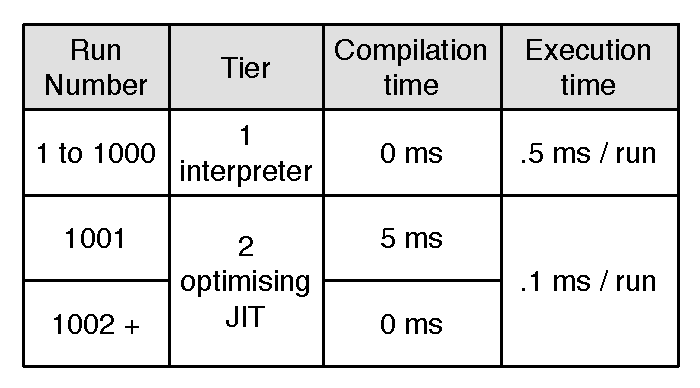
\includegraphics[width=0.5\linewidth]{GeneralTieredArchitecture}
        \caption{Execution of a frequently used code snippet.}
        \label{fig:GeneralTieredArchitecture}
    \end{center}
\end{figure}

\paragraph{Optimising JIT architectures.} Two main architectures are widely used to design an optimising JIT. The first optimising JIT architecture~\cite{UrsPHD}, historically the first one invented, attempts to boost performance by optimising frequently used functions. Such optimising JIT generates native code snippets corresponding to optimised functions. We call this architecture the \emph{Function based architecture} and we describe it in Section \ref{sec:architecture}. The second architecture focuses on the optimisation of linear sequences of frequently used instructions. We call this architecture the \emph{Meta-tracing architecture}. Typically, meta-tracing JITs optimise the common execution path of one iteration of each frequently used loop. This second architecture is detailed in Section \ref{sec:metaArchitecture}. As Sista is more similar to the function based architecture, Section \ref{sec:architecture} is more detailed than the other one.

\paragraph{Research problems.} In the context of the design and implementation of the optimising JIT for Pharo, the thesis focuses on 
two
%three 
aspects:
\begin{itemize}
	\item \emph{Metacircular optimising JITs: } Optimising JITs can be written in different programming languages, including the language they optimise. In the latter case, it may be possible for the JIT to optimise its own code. Such aspects are discussed in Section \ref{sec:implLang}.
	\item \emph{Runtime state persistence:} Most modern VMs always start-up an application with only unoptimised code. The application then needs a certain amount of time, called \emph{warm-up time}, to reach peak performance. Warm-up time is a problem if the application needs high-performance immediately. Existing solutions for this problem are detailed in Section \ref{sec:persistence}.
	%\item \emph{Virtual function instruction set:} Most VMs are either only able to execute code from a specific programming language or from a specific virtual function representation. Several modern VMs are able to execute code in other form, for example
\end{itemize}

%what do we discuss
\paragraph{Closed-source VMs.} This chapter tries to discuss the main production and research open-source VMs. Specific closed-source VMs are described as they are relevant in the context the thesis. However, many closed-source VMs are ignored as it is difficult to get reliable and free-to-share information about them, especially if no publications exist on a specific aspect of the VM. 

%Smalltalk.
\paragraph{Smalltalk VMs.} As Pharo is a Smalltalk dialect, it is relevant to investigate the designs of other Smalltalk VMs. However, commercial Smalltalk VMs in production today are closed-source and do not feature optimising JITs so we do not discuss them. In the 90s, the Self VM~\cite{UrsPHD} and the animorphic VM for Strongtalk~\cite{Sun06} were able to execute Smalltalk code using an optimising JIT. Those VMs are briefly discussed but these VMs are not actively maintained nor used in production.

%%%%%%%%%%%%%%%%%%%%%%%%%%%%%%%%%%%%%%%%%%%%%%%%%%%%%%%%%%%%%%%%%%%%%%%%%%%%%%%%%%%%%%%%%%%%%%%%%%%%%%%%%%%%%%%%%%%%%%%%%%%%%%%%%%%%%%%%%%%%%%%%%%%%%%%%%%%%%%%%%%%%%%%

\section{Terminology}

This section clarifies specific terms to avoid confusion.

\paragraph{Functions.} In the thesis we use the term \emph{function} to refer to executable code, which corresponds in practice to a method or a closure. More specifically, we distinguish \emph{virtual functions}, or v-functions, which can be executed by a virtual machine (in our case, bytecode version of functions) and \emph{native functions}, or n-functions, the native code version of a function executed by a specific processor. 

\paragraph{Frames.} We discuss VMs using a hybrid runtime where v-functions can be executed either through a v-function interpreter or by executing the corresponding n-function generated by a JIT from the v-function. On the one hand, we call \emph{virtual frame} or v-frame a stack frame used by the v-function interpreter. On the other hand, we call \emph{native frame} or n-frame a stack frame used by the execution of a n-function. V-frames have typically a machine-independent representation and all the values used by the execution stored inside the frame, while n-frames may have a machine-dependent representation and may have some values in registers.

\paragraph{Tiered architecture.} One of the most common high-performance VM architectures is the tiered architecture: the first few executions of v-functions are performed by an interpreter and subsequent executions fall into the JIT infrastructure, composed of multiple tiers. Each JIT tier requires more time to compile the v-function to n-function than the previous tier, but the resulting n-function is more efficient. In most VMs, there are two JIT compiler tiers. The first tier is called the \emph{baseline JIT}. It translates quickly v-functions to n-functions with a limited number of optimisations. The baseline JIT typically generates n-functions with inline caches to collect type information. The other tier is called the \emph{optimising JIT}. It translates v-functions to highly optimised n-functions with speculative optimisations, based on the runtime information collected on n-functions generated by the baseline JIT.

\paragraph{Sista.} \emph{Sista} (\textbf{S}peculative \textbf{I}nlining \textbf{S}mall\textbf{T}alk \textbf{A}rchitecture) is the named of the architecture detailed in the thesis. As the architecture has notable differences from the standard tiered architecture, the two runtime compilers are not really a baseline JIT and an optimising JIT. We call them by their project name in the thesis. The first runtime compiler is called \emph{Scorch} and compiles v-functions to optimised v-functions using speculative optimisations. Scorch is written in plain Smalltalk. The second runtime compiler is called \emph{Cogit} and compiles v-functions to n-functions. Cogit can be used alone as the baseline JIT, or as a back-end for Scorch. In the later case, the pair of Scorch and Cogit forms an optimising JIT. Cogit is written in a restrictive Smalltalk compiled ahead-of-time to an executable as part of the VM.

In this context, both v-functions and n-functions can have an optimised version. We therefore used the term v-function to discuss all v-functions (optimised or not), and specify optimised v-function and unoptimised v-function when needed. Similarly, for frames, we say v-frame to discuss v-frames in general, and specify optimised v-frame and unoptimised v-frame when discussing a v-frame respectively representing the execution state of an optimised v-function or a unoptimised v-function. The same terminology is used with native (\emph{n-}) than with virtual (\emph{v-}).

%Both runtime compilers can deoptimise stack frames. Cogit can deoptimise any n-frame to a single v-frame. Scorch can deoptimise an optimised v-frame to multiple unoptimised v-frames. 

%%%%%%%%%%%%%%%%%%%%%%%%%%%%%%%%%%%%%%%%%%%%%%%%%%%%%%%%%%%%%%%%%%%%%%%%%%%%%%%%%%%%%%%%%%%%%%%%%%%%%%%%%%%%%%%%%%%%%%%%%%%%%%%%%%%%%%%%%%%%%%%%%%%%%%%%%%%%%%%%%%%%%%%

\section{Function based architecture}
\label{sec:architecture}

The first optimising JIT architecture invented~\cite{UrsPHD} was designed to generate optimised n-functions. From a given v-function, the optimising JIT performs a set of optimisations which includes inlining of other v-functions, and generates an optimised n-function. The section gives firstly an overview of the architecture and then discuss concrete implementations with references in Section \ref{sec:existing1}. The last sections discuss specific aspects of the architecture.

\subsection{Architecture overview}

In most VMs following this architecture, three tiers are present. The following three paragraphs detail each tier, including how virtual calls are executed in each case.

\paragraph{Tier 1: V-function interpreter. } The first tier is a virtual function interpreter. In most VMs, no compilation time is required at all to interpret a v-function\footnote{Some VMs (such as Strongtalk) require compilation time for interpretation because the v-functions are not provided in a format the interpreter can execute (for example source code is provided).} but the execution of the v-function by the interpreter is not very fast. Virtual calls are usually implemented using a global look-up cache to avoid computing the function to activate at each call. The interpreter tier does not necessarily collect runtime information. 
\paragraph{Tier 2: Baseline JIT. } The second tier is the baseline JIT, which generates from a single v-function a n-function with a very limited number of optimisations. Once compiled, the n-function is used to execute the function instead of interpreting the v-function. A small amount of time is wasted to generate the n-function but the execution of the n-function is faster than the v-function interpretation. The n-function generated by the baseline JIT is introspected to collect runtime information if the function is executed enough times to be optimised by the next tier. The goal of the baseline JIT is therefore to generate n-functions providing reliable runtime information with limited performance overhead and not to generate the most efficent n-functions. Virtual calls are usually generated in machine code using inline caches~\cite{Deut84a,Holz91a}: each virtual call has a local cache with the functions it has activated, both speeding-up the execution and collecting runtime information for the next tier.
\paragraph{Tier 3: Optimising JIT. } The last tier is the optimising JIT, which generates an optimised n-function. The optimising JIT uses runtime information such as the inline cache data to speculate on what function is called at each virtual call, allowing to perform inlining and to generate the optimised n-function from multiple v-functions. Such optimisations greatly speed-up the execution but are invalid if one of the compile-time speculation is not valid at runtime. In this case, the VM deoptimises the code and re-optimises it differently~\cite{Holz94a,Holz92a}. The optimising JIT requires more time than the baseline JIT to generate n-functions, but the generated code is much faster. The execution of virtual calls is not really relevant in this tier as most virtual calls are removed through inlining and most of the remaining ones are transformed to direct calls.

\vspace{0.5em}

\begin{figure}[h!]
    \begin{center}
        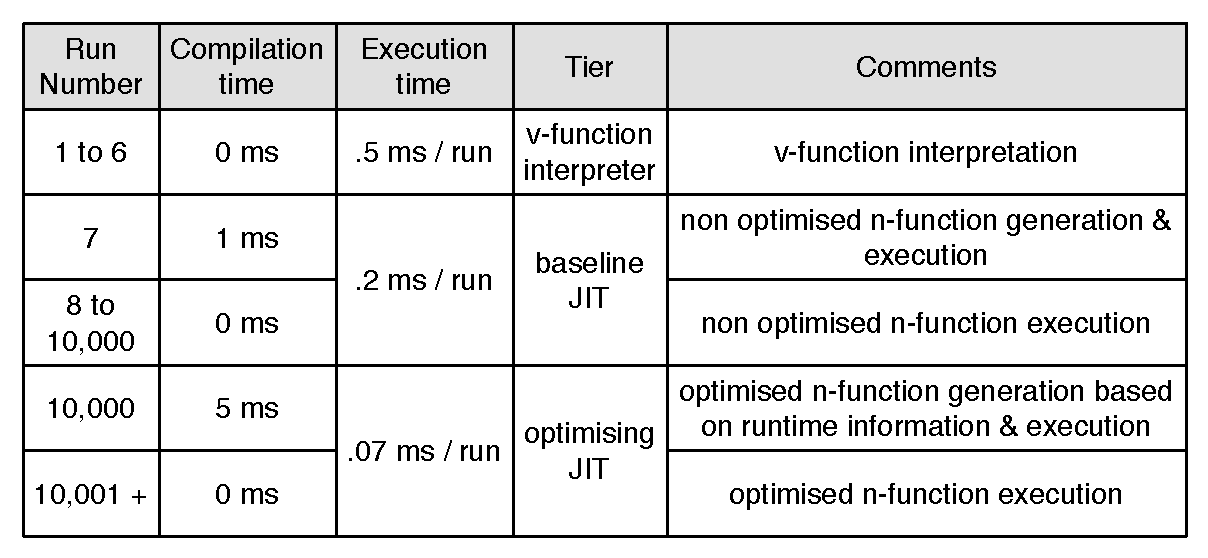
\includegraphics[width=0.95\linewidth]{TieredArchitecture}
        \caption{Execution of a frequently used v-function}
        \label{fig:TieredArchitecture}
    \end{center}
\end{figure}

Figure \ref{fig:TieredArchitecture} shows the theoretical execution of a frequently used v-function over the three tiers. The first few runs are interpreted, each run taking 0.5 ms. The following run requires some compilation time for the baseline JIT to kick in, but the function is then executed 2.5 times faster and runtime information is collected. Lastly, after 10,000 runs, the optimising JIT takes a significant amount of time to generate an optimised n-function. The optimised n-function is executed three times faster than n-function generated by the baseline JIT.

\subsection{Existing virtual machines}
\label{sec:existing1}

The first VM featuring this function based architecture was the Self VM~\cite{UrsPHD}. The Self VM had only two tiers, the baseline JIT and the optimising JIT. %The Self programming language has never really become popular so the VM is not really used anymore. 

The second VM built with this design was the Animorphic VM for the Strongtalk programming language~\cite{Sun06}, a Smalltalk dialect. This VM is the first to feature three tiers. The first tier is a threaded code interpreter hence interpretation requires a small amount of compilation time to generate threaded code from the v-function. The two other tiers are the same as in the Self VM. The animorphic VM has never reached production.

The Hotspot VM~\cite{Pale01a} was implemented from the Self and animorphic VM code base and has been the default Java VM provided by Sun then Oracle for more than a decade. In the first versions of the Hotspot VM, two executables were distributed. One was called the client VM, which included only the baseline JIT and was distributed for applications where start-up performance matters. The other one was called the server VM, which included both JIT tiers, and was distributed for application where peak performance matters. Later, the optimising JIT was introduced in the client VM with different optimisation policies than the server version to improve the client VM performance without decreasing too much start-up performance. In Java 6 and onwards, the server VM became the default VM as new strategies allowed the optimising JIT to improve performance with little impact on start-up performance. Lastly, a single binary is now distributed for the 64 bits release, including only the server VM. 

More recently, multiple Javascript VMs were built with a similar design. A good example is the V8 Javascript engine~\cite{V8}, used to execute Javascript in Google Chrome and Node JS. Other VMs, less popular than the Java and Javascript VMs are also using similar architectures, such as the Dart VM. 

One research project, the Graal compiler~\cite{Oracle13,Dubo13c}, is a function-based optimising JIT for Java that can be used, among multiple use-cases, as an alternative optimising JIT in the Hotspot VM.

\subsection{Just-in-time compiler tiers}

Most VMs featuring a function based architecture in production nowadays have three tiers. The number of tiers may however vary from two to as many as the development team feels like. The following paragraphs discuss the reasons why the VM implementors may choose to implement a VM with two tiers, three tiers or more.

\paragraph{Engineering cost.} Each new tier needs to be maintained and evolved accordingly to the other tiers. Hence, a VM having more tiers requires more engineering time for maintainance and evolutions. Any bug can come from any tier and bugs coming from only a single tier can be difficult to track down. Evolutions need to be implemented on each tier. To lower the VM maintenance and evolution cost, a VM needs to have the least number of tiers possible.

\paragraph{Minimum number of tiers.} By design, the optimising JIT is the key component for high-performance and it needs runtime information from previous runs to generate optimised code. Hence, a VM with a function based architecture requires at least two tiers. One tier, the non-optimising tier, is used for the first runs to collect statistical information and is typically implemented as an interpreter tier or a baseline JIT tier. The second tier, the optimising tier, generates optimised n-functions and is implemented as an optimising JIT. To perform well, the optimising tier has to kick in only if the function is used frequently (else the compilation time would not be worth the execution time saved) and the previous tier(s) must have executed the v-function enough time to have collected reliable runtime information. For this reason, the optimising tier usually kicks in after several thousands executions of the v-function by the previous tier(s).

\paragraph{Two non-optimising tiers.}Most VMs feature two non-optimising tiers and one optimising tier. The non-optimising tiers are composed of an interpreter tier and a baseline JIT tier. These two tiers have different pros and cons and featuring both allows the VM to have the best of both worlds. There are three main differences between the two tiers: execution speed, efficiency of runtime information collection and memory footprint. The three differences are detailed in the next three paragraphs.

\subparagraph{Execution speed.} The interpreter tier is faster than the baseline JIT tier if the function is executed a very small number of times because there are not enough executions to outweight the baseline JIT compilation time. Figure \ref{fig:NonOptTierGraph} compares the speed of one to ten executions of the frequently used v-function from Figure \ref{fig:TieredArchitecture}. As interpreting the v-function takes 0.5 ms, the compilation by the baseline JIT 1 ms and the execution of the n-function generated by the baseline JIT 0.2 ms, the interpreter is faster if the v-function is executed less than three times. However, if the function is executed between four times and 10,000 (at which point the optimising JIT kicks in), the baseline JIT tier is faster.

\begin{figure}[h!]
    \begin{center}
        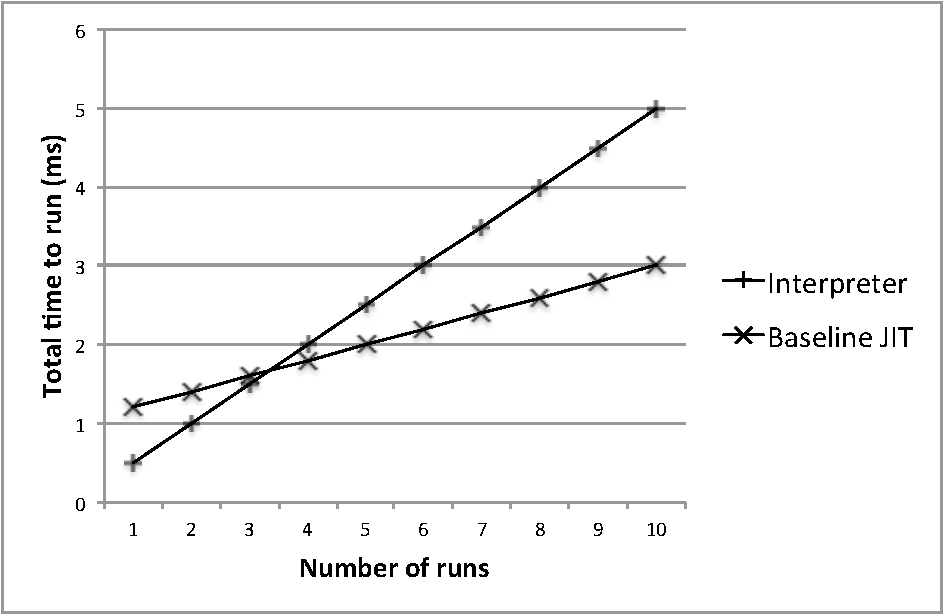
\includegraphics[width=0.70\linewidth]{NonOptTierGraph}
        \caption{Time to execute a v-function in non-optimising tiers}
        \label{fig:NonOptTierGraph}
    \end{center}
\end{figure}
	
	\subparagraph{Runtime information collection.} One of the most relevant runtime information to collect is the function called at each virtual call. It is currently not possible to collect this information without overhead in an interpreter if the interpreter is written in a machine independent language. However, the inline cache technique~\cite{Deut84a,Holz91a} allows one to collect such information in a baseline JIT tier while speeding-up code execution.
	
	\subparagraph{Memory footprint.}The interpreter does not require extra memory for the function it executes as only the v-function representation is needed. On the other hand, the baseline JIT requires memory to store the generated n-function for each v-function it executes. If many functions are executed once, not having the interpreter tier can lead to significant memory overhead.
	
	%\item \emph{Compatibility with optimising JIT: }The code executed by the processor in the interpreter tier is the interpreter code while in the baseline JIT tier is native code. Having both an interpreter and JIT tiers require the runtime to be able to switch efficiently between both runtime, including the management of stack frame representation in both cases.
%\end{enumerate}

\vspace{0.5em}

Having both tiers allows the VM to have a lower memory footprint thanks to the interpreter tier. If the interpreter tier does not collect runtime information and is used only for the first few executions, the start-up performance is much better when both tiers are present than when one or the other is present alone. Runtime information can be collected with little overhead thanks to the baseline JIT tier. For these reasons, many VMs feature these two non-optimising tiers. 

A good example of the pros and cons of multiple tiers is the evolution of the V8 Javascript engine~\cite{V8}. In 2008, the first version was released featuring only the baseline JIT tier. The following year, the optimising JIT tier was added to improve performance. In 2016, the interpreter tier was added both to lower the memory footprint and to improve start-up performance.

In general, the two non-optimising tiers are kept as simple as possible to ease maintainance and evolutions. Only the third tier, the optimising JIT, may be more complex to be able to generate efficient n-functions.

\paragraph{More than three tiers.} Adding more than three tiers is usually not worth it as it would mean additional maintenance and evolution cost. However, in specific languages such as Javascript where the start-up performance is critical, it can be worth it to have two optimising JIT tiers to increase start-up performance. The Javascript Webkit VM has four tiers since 2015~\cite{Webkit15}. In this case, the VM team introduced two optimising JIT tiers after the interpreter and baseline JIT. One optimising JIT tier has smaller compilation time than the other one but produce less efficient n-function.

\paragraph{Independant compiler tiers.}
In most VMs, the baseline JIT and the optimising JIT are completely independant entities. Indeed, both JIT tiers are fundamentally different and it is difficult to share code between both tiers. 

\subparagraph{Baseline JIT.} The baseline JIT has to be as simple as possible to limit the maintenance cost, simplicity is more important than generated code quality as most of the VM performance comes from the optimising JIT. The n-functions it generates need to be easily introspected to collect runtime information about the previous runs for the optimising JIT to direct compiler optimisations. The baseline JIT compilation time has to be very small.

The baseline JIT is typically implemented as a template-based engine~\cite{Deut84a}, generating a predefined sequence of native instructions for each virtual instruction. Template-based generation engines are relatively simple to implement and maintain. Templates are very convenient for native code introspection because the JIT knows the exact sequence of native instructions generated for each virtual instruction so it knows the exact bytes to read to extract runtime information. Lastly, template-based compilation is usually very efficient, providing low compilation time.

\subparagraph{Optimising JIT.} The optimising JIT is significantly different. It needs to generate n-functions as efficient as possible with a reasonnable compilation time, but potentially much higher than the baseline JIT. The n-functions generated by the optimising JIT are not introspected in most VMs, allowing the optimising JIT to generate the most efficient instructions. As any software project, complexity has to be controlled but it is usually worth to add complexity in the optimising JIT to allow it to generate more efficient code as it leads to overall better VM performance. The optimising JIT is typically implemented, as shown in Figure \ref{fig:OptJITFig}, by translating the v-function to a high-level intermediate representation to perform language-specific optimisations. It then transforms the representation to another intermediate representation, closer to native instructions, where machine-specific optimisations are performed. Lastly it generates native code.

\begin{figure}[h!]
    \begin{center}
        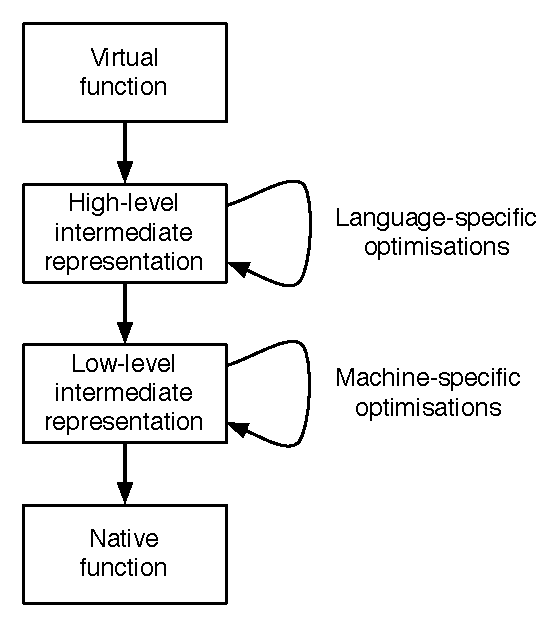
\includegraphics[width=0.49\linewidth]{OptJITFig}
        \caption{Classical optimising JIT architecture}
        \label{fig:OptJITFig}
    \end{center}
\end{figure}

\paragraph{Sharing code between compiler tiers.} Because of the fundamental differences, most optimising JITs use a completely different code base than the baseline JIT they work with. However, there are some rare cases where part of the JIT compilers are shared between multiple tiers. 

The first case is the Javascript Webkit VM~\cite{Webkit15}. As four tiers are present, it is possible to share portions of the compilers because some features are required in multiple tiers. For example, both the baseline JIT and the first-level optimising JIT requires the VM to be able to instrospect the generated machine code. In addition, both optimising JITs have optimisation logic in common allowing to share part of the optimisation pipeline. In this case, they share the high-level optimisations while the low-level optimisations are done in different back-ends.

The second case is related to VM extensions. The Javascript VMs are now attempting to support, in addition of Javascript, an abstract assembly language called WebAssembly~\cite{WebAssembly}. WebAssembly allows the programmer to compile ahead-of-time specific frameworks or libraries for use-cases difficult to optimise efficiently at runtime, such as real-time libraries. WebAssembly provides both abstract assembly code instructions and convenient instructions to interface WebAssembly with Javascript and the web page. In the V8 Javascript engine~\cite{V8}, the low-level intermediate representation of TurboFan, the optimising JIT of V8, is shared between the WebAssembly back-end and the optimisation path for Javascript code.

\subsection{Concurrent compilation}

The first optimising JIT, designed and implemented in Self~\cite{UrsPHD}, was done in a single-threaded environment. In this case, the optimising JIT had a limited time period to produce optimised code, and if the time period was not enough, the function was not optimised. Since the early 2000s, multi-threaded environments have become more common and many optimising JITs now perform optimisations concurrently to the application native thread(s)~\cite{Arn00,Stad12a}.

In most cases, not all the runtime compilations are however done concurrently. The baseline JIT is typically executed in the same native thread than the application. As it has very small compilation time, the compilation time overhead is usually not significant enough to justify concurrent compilation. When a frequently used portion of code is detected, the optimising JIT has to choose a function to optimise based on the current stack. This cannot be done concurrently as the stack needs to be introspected. Once the function to optimise is chosen, the optimisation of the function can be done concurrently. The optimising JIT has usually access to a pool of native threads which take functions to optimise in a compilation queue, optimises them and installs them. Further calls on such functions can use the optimised version installed. The optimising JIT may insert guards to ensure assumptions speculated at compile-time (such as the type of a specific variable) are valid at runtime. If one of the guard fails, the stack needs to be deoptimised to resume with non-optimised code. Deoptimisation of the stack is not done concurrently as the application requires the deoptimisation to be finished to resume execution. 

\subsection{Aosta technical report}

Normally technical reports are not relevant enough to be mentioned, but as Sista is based on the Aosta technical report\cite{Mira02c}, it is definitely worth talking about it.

Aosta is a design sketch for an adaptive optimiser implemented in Smalltalk above a conventional Smalltalk virtual machine (a virtual machine featuring a baseline JIT) with \emph{minor} extensions. Adaptive optimisation are discussed in the sense of Urs H\"olzle \cite{UrsPHD}. The sketch is far from complete, focusing on the interface between the optimiser and the virtual machine, hence outlining a potentially portable architecture where an optimiser written in Smalltalk can be hosted above a range of specific virtual machines. This portability is intended to allow the Smalltalk community to collaborate on the project without having to define and implement a common VM, with all the difficulties of migrating current systems to a new VM, allowing the community to apply the optimiser within the existing systems.  Of course, this architecture still requires significant extensions to the execution machinery of existant VMs but these extensions amount to something far from a rewrite.

The sketch is then detailed in the context of HPS, the VisualWorks VM, which is a second generation implementation of Peter Deutsch's PS Smalltalk~\cite{Deut84a}. The author chose to describe the architecture with this VM as he is familiar with it and the sketch needed (according to the author) to be based on an existing VM to make it as real as possible. The sketch is expected to apply more broadly than just HPS but this is yet to prove. The sketch was, in 2002, functioning as a specification for the HPS implementation. 

%%%%%%%%%%%%%%%%%%%%%%%%%%%%%%%%%%%%%%%%%%%%%%%%%%%%%%%%%%%%%%%%%%%%%%%%%%%%%%%%%%%%%%%%%%%%%%%%%%%%%%%%%%%%%%%%%%%%%%%%%%%%%%%%%%%%%%%%%%%%%%%%%%%%%%%%%%%%%%%%%%%%%%%

\section{Meta-tracing architecture}
\label{sec:metaArchitecture}

The main alternative to the function based architecture is the meta-tracing architecture. Meta-tracing JITs do not optimise entire functions but instead focus on optimising linear sequences of instructions. As most meta-tracing JITs focus on the optimisation of loop iterations, we detail this case in this section. The section starts by providing an overview of the architecture and then discusses concrete implementation with references in Section \ref{sec:existing2}.

\subsection{Architecture overview}

VMs with meta-tracing JITs generate optimised native code only for the frequently used paths of commonly executed loops and interpret virtual instructions for the rest of the program. Tracing JITs are built on the following basic assumptions:
\begin{itemize}
	\item Programs spend most of their runtime in loops.
	\item Several iterations of the same loop are likely to take similar code paths.
\end{itemize}

Typically, in VMs with tracing JITs, the first executions of a loop are done using a v-function interpreter. The interpreter profiles the code executed to detect frequently used loops, usually by having a counter on each backward jump instruction that counts how often this particular backward jump is executed. When a hot loop is identified, the interpreter enters a special mode, called tracing mode. During tracing, the interpreter records a history of all the operations it executes during a single execution of the hot loop. The history recorded by the tracer is called a trace: it is a list of operations, together with their actual operands and results. Such a trace can be used to generate efficient native code. This generated machine code is immediately executable and can be used in the next iteration of the loop.

Being sequential, the trace represents only one of the many possible paths through the code. To ensure correctness, the trace contains a guard at every possible point where the path could have followed another direction, for example at conditional branches or virtual calls. When generating native code, every guard is turned into a quick check to guarantee that the path we are executing is still valid. If a guard fails, the execution immediately quits the native code and resumes the execution by falling back to the interpreter.

\subsection{Existing VMs}
\label{sec:existing2}

Tracing optimisations were initially explored by the Dynamo project~\cite{Bala00a} to dynamically optimise native code at runtime. Its techniques were then successfully used to implement a JIT compiler for a Java VM~\cite{Gal06a}. The technique was used in Mozilla's JavaScript VM from Firefox 3 to Firefox 11~\cite{Gal09a} until Mozilla removed it to replace it by a function-based JIT. 

The most famous meta-tracing JITs in production are certainly the ones generated from the RPython toolchain~\cite{Rigo06a}. The RPython toolchain allows the generation of a meta-tracing JIT for free if one writes a virtual function interpreter in RPython. The most popular example is Pypy~\cite{Rigo06a,PyPyTracing}, a Python VM using a meta-tracing JIT through the RPython toolchain framework.

\subsection{Sista and metatracing JITs}

Sista was not designed as a metatracing JIT. There were two main reasons. First, the design was inspired from the Aosta proposal, which is a function-based architecture design. Second, we did not believe that optimising loop bodies would make sense in the context of Smalltalk and we will explain why in the second paragraph of Section \ref{sec:relWArch}.

%%%%%%%%%%%%%%%%%%%%%%%%%%%%%%%%%%%%%%%%%%%%%%%%%%%%%%%%%%%%%%%%%%%%%%%%%%%%%%%%%%%%%%%%%%%%%%%%%%%%%%%%%%%%%%%%%%%%%%%%%%%%%%%%%%%%%%%%%%%%%%%%%%%%%%%%%%%%%%%%%%%%%%%

\section{Metacircular optimising Just-in-time compiler}
\label{sec:implLang}

An optimising JIT is implemented in a programming language and is able to optimise code from one or multiple programming languages. If the implementing language of the optimising JIT is one of the language it can optimise, is the optimising JIT able to optimise its own code ?

The section starts by discussing the programming languages in which the optimising JITs are written. For the rare case where the implementing language of an optimising JIT is included in the languages the JIT can optimise, we detail if such optimisations are possible and used in production.

\subsection{Implementation language}
Historically, VMs have been implemented in low-level languages such as C++. Low-level languages are very convenient for multiple VM development tasks, such as direct memory access or optimisation of specific portion of the VM code for performance. The first optimising JITs, including the Self, Animorphic and Java Hotspot VMs~\cite{UrsPHD,Sun06} were written in C++. More recently, Javascript VMs such as V8 or Webkit~\cite{Webkit15} were still written in C++. As far as we know, there is no optimising JIT in production optimising C++ code, hence none of these JITs are able to optimise their own code.

Another approach is to use a high-level language compiled ahead-of-time to assembly code to write the optimising JIT. This approach is used by the RPython toolchain~\cite{Rigo06a}, where RPython is a restricted Python that can be compiled to native code through C. RPython was used to write Pypy's meta-tracing optimising JIT. In the case of Pypy, the JIT is able to optimise Python code, and as RPython is a subset of Python, the JIT is able to optimise its own code. However, in production, all the RPython code is compiled ahead-of-time to an executable binary. All the JIT code base is therefore translated to native code, and as the JIT cannot optimise native code, the JIT does not optimise itself in production.

Figure \ref{fig:RPythonVMCompilation} shows the compilation of the production VM using RPython. The Core VM is written in RPython, and the RPython to C compiler generates C files from the RPython code. The final VM is compiled using a C compiler from the generated C files and additional C files for platform-specific code.

\begin{figure}[h!]
    \begin{center}
        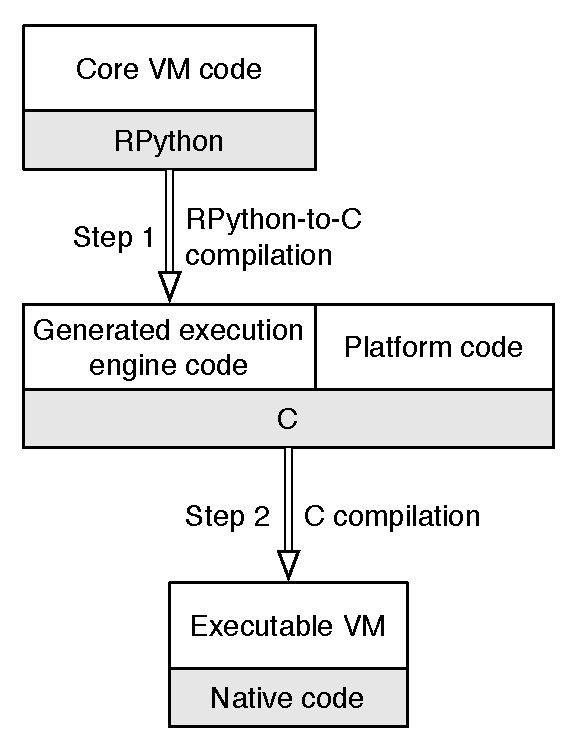
\includegraphics[width=0.45\linewidth]{RPythonVMCompilation}
        \caption{RPython VM executable generation}
        \label{fig:RPythonVMCompilation}
    \end{center}
\end{figure}

\paragraph{Metacircular VMs.} Multiple research projects showed that it is possible to implement an entire VM in the programming language the VM runs. Such VMs are called metacircular VMs. 

The Jalape\~no project, now called Jikes RVM~\cite{Alp99a}, was the first successful VM with such a design. Jikes RVM is a Java VM written in Java. On the Jikes RVM official page, it is written that the current version of the VM does not perform runtime optimisations based on runtime information. There is however a runtime compiler present in Jikes RVM~\cite{Arn00} optimising the code more aggressively than the baseline JIT, but it does not seem to use runtime information to direct its optimisations. 

%TODO Disambig metacircular VM.

Another Java VM written in Java was implemented in the late 2000s at Oracle, called Maxine VM~\cite{Wimm13a}. Maxine had multiple working optimising JITs. The most popular was extracted from the Maxine VM and is now known as the Graal compiler~\cite{Oracle13,Dubo13c}. In the case of Maxine, the optimising JIT is written in Java and is able to optimise its own code.

There were other attempts to implement meta-circular VMs for other languages than Java. The Klein VM~\cite{Unga05b} is a Self VM written in Self and reportedly, in 2009, there was some work in the direction of an optimising JIT. The project does not seem however to be very active today and the optimising JIT is definitely not fully working. There is even an attempt to write a Smalltalk VM in Smalltalk~\cite{Pim14a}, called Bee Smalltalk. Unfortunately, as of today, Bee Smalltalk is not open-source and it is not clear if an optimising JIT is present or not.

The last but not least project is the Truffle framework~\cite{Wur13a}. Truffle is a framework allowing to write efficiently VMs for different programming languages. The Truffle runtime is built on top of Java's Hotspot VM, but the Graal compiler is used as the optimising JIT instead of the Hotspot optimising compiler. 
Multiple VMs using the Truffle framework were implemented for different programming language in the past years. For each of them, the Graal compiler in the Truffle runtime can optimise both Java code and the programming language run. As Graal is written in Java, it can optimise its own code.
 
\subsection{Optimising Just-in-time compiler optimising itself}

Overall, very few optimising JITs are written in a programming language they can optimise. Even when they could optimise themselves, the VM development team may choose to compile the JIT code to native code ahead-of-time and the optimising JIT does not optimise itself in production. The main existing case where the optimising JIT is optimising its own code is the Graal optimising JIT. Graal can be used in different contexts. It was built as the Maxine VM optimising JIT. It is now mainly used as the optimising JIT of the Truffle runtime, as an alternative optimising JIT for Java Hotspot.

We detail here briefly how the Graal compiler optimise its own code when it is running as an alternative optimising JIT in the Java Hotspot VM. In this case, the Graal optimising JIT is written in Java while the rest of the VM, originally from the Java Hotspot VM, are written in C++. The application is running using multiple native threads and the Graal compiler is running in other native threads, concurrently.

When a frequently used portion of code is detected, the Hotspot VM chooses a function to optimise based on the current stack. The VM then puts the function to optimise in a thread-safe compilation queue. The Graal compiler native threads, running concurrently to the application, take functions to optimise from the compilation queue and generate an optimised function for each function in the queue. Hotspot provides APIs to extract runtime information from each unoptimised function to direct the compiler optimisation. Once the optimisation finished, the Graal compiler provides to Hotspot an optimised n-function with deoptimisation metadata. The Hotspot VM installs the optimised n-function. If one of the compilation-time assumption is invalid at runtime, the Hotspot VM is able to deoptimise the stack based on the deoptimisation metadata provided by the Graal compiler.

%%%%%%%%%%%%%%%%%%%%%%%%%%%%%%%%%%%%%%%%%%%%%%%%%%%%%%%%%%%%%%%%%%%%%%%%%%%%%%%%%%%%%%%%%%%%%%%%%%%%%%%%%%%%%%%%%%%%%%%%%%%%%%%%%%%%%%%%%%%%%%%%%%%%%%%%%%%%%%%%%%%%%%%

\section{Runtime state persistence}
\label{sec:persistence}

In Sista, we persist the runtime state across multiple start-ups, including the optimised code but also the running green threads using optimised code. Persistence of running green threads with optimised code has not been done before to the best of our knowledge. In our case, we need to persist green threads as the normal Smalltalk developer workflow requires it. It seems no other programming language with an optimising JIT have the same requirement so the running green threads are not persisted across start-ups. For this reason, we focus in this section on the persistence of optimised code between multiple start-ups.

One of the main problems with optimising JITs, compared to ahead-of-time compiler, is the start-up performance. As the optimising JIT needs runtime information to optimise code, usually thousands of unoptimised runs of a code snippet are required before reaching peak performance. This warm-up time can cause significant problems in specific short-lived applications, where most of the execution time is spent before reaching peak performance. 
%In addition, the warm-up time implies additional energy consumption (the processor needs to optimise code, consuming energy) at each application start-up, which is a problem in specific use-cases such as mobiles where battery consumption is critical.

Because of these constraints, some object-oriented languages are compiled with an ahead-of-time compiler. Static analysis is performed over the code to guess what function is called at each virtual call. Applications for the iPhone are a good example where static analysis is used to pre-optimise the Objective-C application. The peak performance is lower than with a JIT compiler if the program uses a lot of virtual calls, as static analysis is not as precise as runtime information on highly dynamic languages. However, if the program uses few dynamic features (for example most of the calls are not virtual) and is running on top of a high-performance language kernel like the Objective-C kernel, the result can be satisfying.

Most object-oriented languages still choose to run on top of a VM with an optimising JIT. The section describes four existing techniques to improve start-up performance, including techniques related to optimised code persistence across start-ups.

\paragraph{Many tiers architecture.}
One solution to decrease warm-up time is to have many tiers in the function based architecture. The idea is that code would be executed slowly the few first iterations, a bit faster the next iterations, faster after an certain number of optimisations, and so on. Instead of being slow for many iterations before being fast, the VM can this way have a very good trade off between compilation time, runtime information quality and code performance.

The best example is the Javascript Webkit VM~\cite{Webkit15}. A code snippet is:
\begin{enumerate}
\item Interpreted by a bytecode interpreter the first 6 executions.
\item Compiled to machine code at 7th execution, with a non-optimising compiler, and executed as machine code up to 66 executions.
\item Recompiled to more optimised machine code at 67th execution, with an optimizing compiler doing some but not all optimisations, up to 666 executions.
\item Recompiled to heavily optimised machine code at 667th execution, with all the optimisations.
\end{enumerate}

At each step, the compilation time is greater but the execution time decreases. The many tiers approach (four tiers in the case of Webkit), allows the VM to have decent performance during start-up, while reaching high performance for long running code. However, this technique has a severe drawback: the VM team needs to maintain and evolve many different tiers.

\paragraph{Persisting runtime information.}

To quickly reach peak performance, one way is to save the runtime information, especially inlining decisions made by the optimising JIT. In 
 \cite{Sun06}, it is possible to save the inlining decisions of the optimising compiler in a separate file. The optimising compiler can then reuse this file to take the right inlining decision in subsequent start-ups. In \cite{Arno05c}, the profiling information of unoptimised runs is persisted in a repository shared by multiple VMs, so new runs of the VM can re-use the information to direct compiler optimisations.

\paragraph{Persisting machine code.}

In the Azul VM Zing~\cite{Azul}, available for Java, the official web site claims that "operations teams can save accumulated optimizations from one day or set of market conditions for later reuse" thanks to the technology called \emph{Ready Now!}. In addition, the website precises that the Azul VM provides an API for the developer to help the JIT to make the right optimisation decisions. 

As Azul is closed source, implementation details are not entirely known. However, word has been that the Azul VM reduces the warm-up time by saving machine code across multiple start-ups. If the application is started on another processor, then the saved machine code is simply discarded. It is very difficult to persist optimised native code across multiple start-ups due to position dependent code and low-level details, but with the example of Azul, we know it is possible.

Aside from Azul, the work of Reddi and all~\cite{Redd07a} details how they persist the machine code generated by the optimising JIT across multiple start-ups of the VM. JRockit~\cite{JRockit}, an Oracle product, is a production Java VM allowing to persist the machine code generated by the optimising JIT across multiple start-ups.

\paragraph{Preheating through snapshots.} This paragraph discusses the persistence of the runtime state in snapshots in Dart and in a specifc Java VM.

\paragraph{Dart snapshots.}
The Dart programming language features snapshots for fast application start-up. In Dart, the programmer can generate different kind of snapshots \cite{Anna13a}. The Dart team added in 2016 two new kind of snapshots, specialized for iOS and Android application deployment.

\subparagraph{Android.} A Dart snapshot for an Android application is a complete representation of the application code and the heap once the application code has been loaded but before the execution of the application. The Android snapshots are taken after a warm-up phase to be able to record call site caches in the snapshot. The call site cache is a regular heap object accessed from machine code, and its presence in the snapshot allows one to persist type feedback and call site frequency. %Call sites are filled ahead ot time by simulating the execution of the application.

\subparagraph{iOS.} For iOS, the Dart snapshot is slightly different as the platform does not allow JIT compilers. All reachable functions from the iOS application are compiled ahead of time, using only the features of the Dart optimising compiler that don't require dynamic deoptimisation. A shared library is generated, including all the instructions, and a snapshot that includes all the classes, functions, literal pools, call site caches, etc.

\paragraph{Cloneable VMs.}
In Java, snapshots are not available and used by default. However, Kawachiya and all describe in their work~\cite{Kawa07a} extensions to a Java VM to be able to clone the state of a running Java VM in a similar way to snapshots. In this work, the cloned VM duplicates the heap but also the machine code generated by the different JIT tiers.

%%%%%%%%%%%%%%%%%%%%%%%%%%%%%%%%%%%%%%%%%%%%%%%%%%%%%%%%%%%%%%%%%%%%%%%%%%%%%%%%%%%%%%%%%%%%%%%%%%%%%%%%%%%%%%%%%%%%%%%%%%%%%%%%%%%%%%%%%%%%%%%%%%%%%%%%%%%%%%%%%%%%%%%

%\section{Virtual machine interface}

%\subsection{The Graal-Hotspot architecture}

%+ Graal and interface

%\subsection{WebAssembly}

%WebAssembly 

%%%%%%%%%%%%%%%%%%%%%%%%%%%%%%%%%%%%%%%%%%%%%%%%%%%%%%%%%%%%%%%%%%%%%%%%%%%%%%%%%%%%%%%%%%%%%%%%%%%%%%%%%%%%%%%%%%%%%%%%%%%%%%%%%%%%%%%%%%%%%%%%%%%%%%%%%%%%%%%%%%%%%%%

\section*{Conclusion} 

This chapter detailed existing solutions for our research problems, including the existing optimising JIT architectures, their implementation languages and how some VMs persist optimised code across multiple start-ups. The following chapter describes the existing Pharo runtime which was used as a starting point for our implementation.

%%%%%%%%%%%%%%%%%%%%%%%%%%%%%%%%%%%%%%%%%%%%%%%%%%%%%%%%%%%%%%%%%%%%%%%%%%%%%%%%%%%%%%%%%%%%%%%%%%%%%%%%%%%%%%%%%%%%%%%%%%%%%%%%%%%%%%%%%%%%%%%%%%%%%%%%%%%%%%%%%%%%%%%

%FOLLOWING IS OLD VERSION FOR HISTORY.

%In this chapter, the most popular production VMs and relevant research VMs are discussed. In further chapter, the thesis' proposed architecture will be compared against those VMs. 

%Most popular production VMs, such as Java Hotspot (Cite) or Javascript's V8 (Cite) VMs are written in C++. Using C++ as a performance oriented low-level programming language proved to be very effective as it is possible to write code in a performance oriented fashion. A clear separation is made between the VM and the programming language run so there are no metacircular problems.

%Most of those VMs start-up from the language kernel, a set of core librairies and either source files or files containing bytecodes. Reaching peak performance takes a certain amount of time as the VM needs to detect and optimise correctly frequently used patterns of code. Reportedly, this warm-up time can be from several milliseconds up to multiple days. To solve partially the warm-up problem, such VMs are built with a tiered-architecture: the first few executions are run slowly but without any compilation time, subsequent hundreds of executing are run a bit faster with limited compilation time while further execution are run at peak performance after a certain amount of compilation time.

%An interesting point ot note is that several mainstream VMs were led by the same person (Lars Bak), who became very good at implementing very efficient and easy-to-maintain VMs in C++ as he implemented multiple of those in his life. His work therefore pushed the direction of VM implementation in the C++ direction.

%Among the C++ virtual machines, we will detail two specific VMs have uncommon features that are relevant in the context of the thesis. 

%\subsection{Azul}
%The Azul VM \cite{Azul} is a closed-source VM and expensive VM for Java. As for all closed-source projects, no one external to the project can be certain of what the code is doing. However, word has been that the Azul VM is able to persist optimised machine code across multiple start-ups. If the application is started on another processor, then the saved machine code is simply discarded. 

%\subsection{Dart}
%The Dart VM is an open-source VM for the Dart programming language. Dart features snapshots for fast application start-up. In Dart, the programmer can generate different kind of snapshots \cite{Anna13a}. Since that publication, the Dart team have added two new kind of snapshots, specialized for iOS and Android application deployment, which are quite similar to our snapshots.


%As the sista architecture is implemented in the context of Smalltalk, it could be relevant to discuss existing Smalltalk virtual machines. These VMs are interesting for multiple reasons, but unfortunately many of the Smalltalk virtual machines in production today are closed-source, making the discussion around them not that relevant as information is missing and unaccessible. In addition, as far as we know, there are no production Smalltalk VM today with an optimising JIT compiler, so the comparison with such VMs is even less relevant. 

%However, speculative optimisations in VMs started with the Self VM (CITE), with Self being a Smalltalk-like language, and was followed up with the strongtalk VM (CITE). Both VMs are open-source and available today but none of them are used in production. Self had never really broken through mainstream programming while strongtalk had never reached production state.

\ifx\wholebook\relax\else
    \end{document}
\fi
\ifx\wholebook\relax\else

% --------------------------------------------
% Lulu:

    \documentclass[a4paper,12pt,twoside]{../includes/ThesisStyle}

	\usepackage[T1]{fontenc} %%%key to get copy and paste for the code!
%\usepackage[utf8]{inputenc} %%% to support copy and paste with accents for frnehc stuff
\usepackage{times}
\usepackage{ifthen}
\usepackage{xspace}
\usepackage{alltt}
\usepackage{latexsym}
\usepackage{url}            
\usepackage{amssymb}
\usepackage{amsfonts}
\usepackage{amsmath}
\usepackage{stmaryrd}
\usepackage{enumerate}
\usepackage{cite}
%\usepackage[pdftex,colorlinks=true,pdfstartview=FitV,linkcolor=blue,citecolor=blue,urlcolor=blue]{hyperref}
\usepackage{xspace}
%\usepackage{graphicx}
\usepackage{subfigure}
\usepackage[scaled=0.85]{helvet}
        
        
\newcommand{\sepe}{\mbox{>>}}
\newcommand{\pack}[1]{\emph{#1}}
\newcommand{\ozo}{\textsc{oZone}\xspace}
\newcommand\currentissues{\par\smallskip\textbf{Current Issues -- }}

\newboolean{showcomments}
\setboolean{showcomments}{true}
\ifthenelse{\boolean{showcomments}}
  {\newcommand{\bnote}[2]{
	\fbox{\bfseries\sffamily\scriptsize#1}
    {\sf\small$\blacktriangleright$\textit{#2}$\blacktriangleleft$}
    % \marginpar{\fbox{\bfseries\sffamily#1}}
   }
   \newcommand{\cvsversion}{\emph{\scriptsize$-$Id: macros.tex,v 1.1.1.1 2007/02/28 13:43:36 bergel Exp $-$}}
  }
  {\newcommand{\bnote}[2]{}
   \newcommand{\cvsversion}{}
  } 


\newcommand{\here}{\bnote{***}{CONTINUE HERE}}
\newcommand{\nb}[1]{\bnote{NB}{#1}}
\newcommand{\fix}[1]{\bnote{FIX}{#1}}
%%%% add your own macros 

\newcommand{\sd}[1]{\bnote{Stef}{#1}}
\newcommand{\ja}[1]{\bnote{Jannik}{#1}}
\newcommand{\na}[1]{\bnote{Nico}{#1}}
%%% 


\newcommand{\figref}[1]{Figure~\ref{fig:#1}}
\newcommand{\figlabel}[1]{\label{fig:#1}}
\newcommand{\tabref}[1]{Table~\ref{tab:#1}}
\newcommand{\layout}[1]{#1}
\newcommand{\commented}[1]{}
\newcommand{\secref}[1]{Section \ref{sec:#1}}
\newcommand{\seclabel}[1]{\label{sec:#1}}

%\newcommand{\ct}[1]{\textsf{#1}}
\newcommand{\stCode}[1]{\textsf{#1}}
\newcommand{\stMethod}[1]{\textsf{#1}}
\newcommand{\sep}{\texttt{>>}\xspace}
\newcommand{\stAssoc}{\texttt{->}\xspace}

\newcommand{\stBar}{$\mid$}
\newcommand{\stSelector}{$\gg$}
\newcommand{\ret}{\^{}}
\newcommand{\msup}{$>$}
%\newcommand{\ret}{$\uparrow$\xspace}

\newcommand{\myparagraph}[1]{\noindent\textbf{#1.}}
\newcommand{\eg}{\emph{e.g.,}\xspace}
\newcommand{\ie}{\emph{i.e.,}\xspace}
\newcommand{\ct}[1]{{\textsf{#1}}\xspace}


\newenvironment{code}
    {\begin{alltt}\sffamily}
    {\end{alltt}\normalsize}

\newcommand{\defaultScale}{0.55}
\newcommand{\pic}[3]{
   \begin{figure}[h]
   \begin{center}
   \includegraphics[scale=\defaultScale]{#1}
   \caption{#2}
   \label{#3}
   \end{center}
   \end{figure}
}

\newcommand{\twocolumnpic}[3]{
   \begin{figure*}[!ht]
   \begin{center}
   \includegraphics[scale=\defaultScale]{#1}
   \caption{#2}
   \label{#3}
   \end{center}
   \end{figure*}}

\newcommand{\infe}{$<$}
\newcommand{\supe}{$\rightarrow$\xspace}
\newcommand{\di}{$\gg$\xspace}
\newcommand{\adhoc}{\textit{ad-hoc}\xspace}

\usepackage{url}            
\makeatletter
\def\url@leostyle{%
  \@ifundefined{selectfont}{\def\UrlFont{\sf}}{\def\UrlFont{\small\sffamily}}}
\makeatother
% Now actually use the newly defined style.
\urlstyle{leo}



	\usepackage{amsmath,amssymb}             % AMS Math
% \usepackage[french]{babel}
\usepackage[latin1]{inputenc}
\usepackage[T1]{fontenc}
\usepackage[left=1.5in,right=1.3in,top=1.1in,bottom=1.1in,includefoot,includehead,headheight=13.6pt]{geometry}
\renewcommand{\baselinestretch}{1.05}

\usepackage{multicol}

% Table of contents for each chapter

\usepackage[nottoc, notlof, notlot]{tocbibind}
\usepackage{minitoc}
\setcounter{minitocdepth}{1}
\mtcindent=15pt
% Use \minitoc where to put a table of contents

\usepackage{enumitem}

\usepackage{aecompl}

% Glossary / list of abbreviations

%\usepackage[intoc]{nomencl}
%\renewcommand{\nomname}{List of Abbreviations}
%
%\makenomenclature

% My pdf code

\usepackage[pdftex]{graphicx}
\usepackage[a4paper,pagebackref,hyperindex=true]{hyperref}

\usepackage{pgfplotstable,booktabs,colortbl}
\pgfplotsset{compat=1.8}

% Links in pdf
\usepackage{color}
\definecolor{linkcol}{rgb}{0,0,0.4} 
\definecolor{citecol}{rgb}{0.5,0,0} 

% Change this to change the informations included in the pdf file

% See hyperref documentation for information on those parameters

\hypersetup
{
bookmarksopen=true,
pdftitle="Sista: a Metacircular Architecture for Runtime Optimisation Persistence",
pdfauthor="Clement BERA", 
pdfsubject="Thesis", %subject of the document
%pdftoolbar=false, % toolbar hidden
pdfmenubar=true, %menubar shown
pdfhighlight=/O, %effect of clicking on a link
colorlinks=true, %couleurs sur les liens hypertextes
pdfpagemode=None, %aucun mode de page
pdfpagelayout=SinglePage, %ouverture en simple page
pdffitwindow=true, %pages ouvertes entierement dans toute la fenetre
linkcolor=linkcol, %couleur des liens hypertextes internes
citecolor=citecol, %couleur des liens pour les citations
urlcolor=linkcol %couleur des liens pour les url
}

% definitions.
% -------------------

\setcounter{secnumdepth}{3}
\setcounter{tocdepth}{1}

% Some useful commands and shortcut for maths:  partial derivative and stuff

\newcommand{\pd}[2]{\frac{\partial #1}{\partial #2}}
\def\abs{\operatorname{abs}}
\def\argmax{\operatornamewithlimits{arg\,max}}
\def\argmin{\operatornamewithlimits{arg\,min}}
\def\diag{\operatorname{Diag}}
\newcommand{\eqRef}[1]{(\ref{#1})}

\usepackage{rotating}                    % Sideways of figures & tables
%\usepackage{bibunits}
%\usepackage[sectionbib]{chapterbib}          % Cross-reference package (Natural BiB)
%\usepackage{natbib}                  % Put References at the end of each chapter
                                         % Do not put 'sectionbib' option here.
                                         % Sectionbib option in 'natbib' will do.
\usepackage{fancyhdr}                    % Fancy Header and Footer

% \usepackage{txfonts}                     % Public Times New Roman text & math font
  
%%% Fancy Header %%%%%%%%%%%%%%%%%%%%%%%%%%%%%%%%%%%%%%%%%%%%%%%%%%%%%%%%%%%%%%%%%%
% Fancy Header Style Options

\pagestyle{fancy}                       % Sets fancy header and footer
\fancyfoot{}                            % Delete current footer settings

%\renewcommand{\chaptermark}[1]{         % Lower Case Chapter marker style
%  \markboth{\chaptername\ \thechapter.\ #1}}{}} %

%\renewcommand{\sectionmark}[1]{         % Lower case Section marker style
%  \markright{\thesection.\ #1}}         %

\fancyhead[LE,RO]{\bfseries\thepage}    % Page number (boldface) in left on even
% pages and right on odd pages
\fancyhead[RE]{\bfseries\nouppercase{\leftmark}}      % Chapter in the right on even pages
\fancyhead[LO]{\bfseries\nouppercase{\rightmark}}     % Section in the left on odd pages

\let\headruleORIG\headrule
\renewcommand{\headrule}{\color{black} \headruleORIG}
\renewcommand{\headrulewidth}{1.0pt}
\usepackage{colortbl}
\arrayrulecolor{black}

\fancypagestyle{plain}{
  \fancyhead{}
  \fancyfoot{}
  \renewcommand{\headrulewidth}{0pt}
}

\usepackage{algorithm}
\usepackage[noend]{algorithmic}

%%% Clear Header %%%%%%%%%%%%%%%%%%%%%%%%%%%%%%%%%%%%%%%%%%%%%%%%%%%%%%%%%%%%%%%%%%
% Clear Header Style on the Last Empty Odd pages
\makeatletter

\def\cleardoublepage{\clearpage\if@twoside \ifodd\c@page\else%
  \hbox{}%
  \thispagestyle{empty}%              % Empty header styles
  \newpage%
  \if@twocolumn\hbox{}\newpage\fi\fi\fi}

\makeatother
 
%%%%%%%%%%%%%%%%%%%%%%%%%%%%%%%%%%%%%%%%%%%%%%%%%%%%%%%%%%%%%%%%%%%%%%%%%%%%%%% 
% Prints your review date and 'Draft Version' (From Josullvn, CS, CMU)
\newcommand{\reviewtimetoday}[2]{\special{!userdict begin
    /bop-hook{gsave 20 710 translate 45 rotate 0.8 setgray
      /Times-Roman findfont 12 scalefont setfont 0 0   moveto (#1) show
      0 -12 moveto (#2) show grestore}def end}}
% You can turn on or off this option.
% \reviewtimetoday{\today}{Draft Version}
%%%%%%%%%%%%%%%%%%%%%%%%%%%%%%%%%%%%%%%%%%%%%%%%%%%%%%%%%%%%%%%%%%%%%%%%%%%%%%% 

\newenvironment{maxime}[1]
{
\vspace*{0cm}
\hfill
\begin{minipage}{0.5\textwidth}%
%\rule[0.5ex]{\textwidth}{0.1mm}\\%
\hrulefill $\:$ {\bf #1}\\
%\vspace*{-0.25cm}
\it 
}%
{%

\hrulefill
\vspace*{0.5cm}%
\end{minipage}
}

\let\minitocORIG\minitoc
\renewcommand{\minitoc}{\minitocORIG \vspace{1.5em}}

\usepackage{multirow}
\usepackage{slashbox}

\newenvironment{bulletList}%
{ \begin{list}%
	{$\bullet$}%
	{\setlength{\labelwidth}{25pt}%
	 \setlength{\leftmargin}{30pt}%
	 \setlength{\itemsep}{\parsep}}}%
{ \end{list} }

\newtheorem{definition}{D�finition}
\renewcommand{\epsilon}{\varepsilon}

% centered page environment

\newenvironment{vcenterpage}
{\newpage\vspace*{\fill}\thispagestyle{empty}\renewcommand{\headrulewidth}{0pt}}
{\vspace*{\fill}}



	\graphicspath{{.}{../figures/}}
	\begin{document}
\fi

\chapter{Existing Pharo runtime}
\label{chap:existing}
\minitoc

%global intro
This chapter describes the Smalltalk dialect Pharo~\cite{Blac09a} and part of its implementation. The Sista architecture was originally designed to improve the performance of the Pharo VM by adding an optimising JIT. Some existing features and implementation details already present in Pharo impacted design decisions. They are detailled in this chapter to help the reader understanding the design decisions explained in further chapters. The chapter is not meant to explain the whole existing implementation, but only the most relevant points for the thesis. 

Pharo is a pure object-oriented language. Everything is an object, including green threads, classes, method dictionaries or virtual functions. It is dynamically-typed and every call is a virtual call. The virtual machine relies on a virtual function interpreter and a baseline JIT named \emph{Cogit} to gain performance. Pharo directly inherits from Smalltalk-80~\cite{Gold83a} but has additionnal features such as real closures, exceptions or continuations.

The chapter successively describes some aspects of the Pharo VM, the interface with the language and the Pharo programming language.

%%%%%%%%%%%%%%%%%%%%%%%%%%%%%%%%%%%%%%%%%%%%%%%%%%%%%%%%%%%%%%%%%%%%%%%%%%%%%%%%%%%%%%%%%%%%%%%%%%%%%%%%%%%%%%%%%%%%%%%%%%%%%%

\section{Virtual machine}

The Pharo VM is a flavor of the Cog VM~\cite{Mira08a}. It relies on a v-function interpreter and Cogit, the baseline JIT, to gain performance.

\paragraph{Executable generation.}
Most of the existing VM, inheriting from the original Squeak VM~\cite{Inga97a}, is written in Slang, a subset of Smalltalk. Slang is compiled to C and then to native code through standard C compilers. The execution engine (the memory manager, the interpreter and the baseline JIT) are entirely written in Slang.

In addition to providing some abstractions over machine-specific-details, the slang code has two main advantages over plain C:
\begin{itemize}
	\item \emph{Specifying inlining and code duplication:} To keep the interpreter code efficient, one has to be very careful on what code is inlined in the main interpreter loop and what code is not. In addition, for performance, specific code may need to be duplicated. For example, the interpreter code to push a temporary variable on stack is duplicated 17 times. The 16 first versions are dedicated versions for temporary numbers 0 to 15, the most common cases, and are more efficient because of the use of constants. The 17th version is the generic version, which could be used on any temporary variable but is used in practice for temporary variable 16 and over. Slang allows to annotate functions to direct Slang to C compilation, by duplicating or inlining specific functions. This feature is very important for uncommon processors where available C compilers are often not as good at optimising C code as on mainstream processors.
	\item \emph{Simulation:} As Slang is a subset of Smalltalk, it can be executed as normal Smalltalk code. This is used to simulate the interpreter and garbage collector behavior. The JIT runtime is simulated using both Slang execution and external processor simulators. Simulation is very convenient to debug the VM as all the Smalltalk debugging tools are available. In addition, the simulator state can be saved and duplicated, which is very convenient to reproduce quickly and many times the same bug happing from a specific runtime state.
\end{itemize}

The executable is generated in two steps as shown on figure \ref{fig:VMCompilation}. The first step is to generate the two C files representing the whole execution engine written in Slang using the Slang-to-C compiler. During the second step, a C compiler is called to compile the execution engine and the platform-specific code written directly in C to the executable VM.

\begin{figure}[h!]
    \begin{center}
        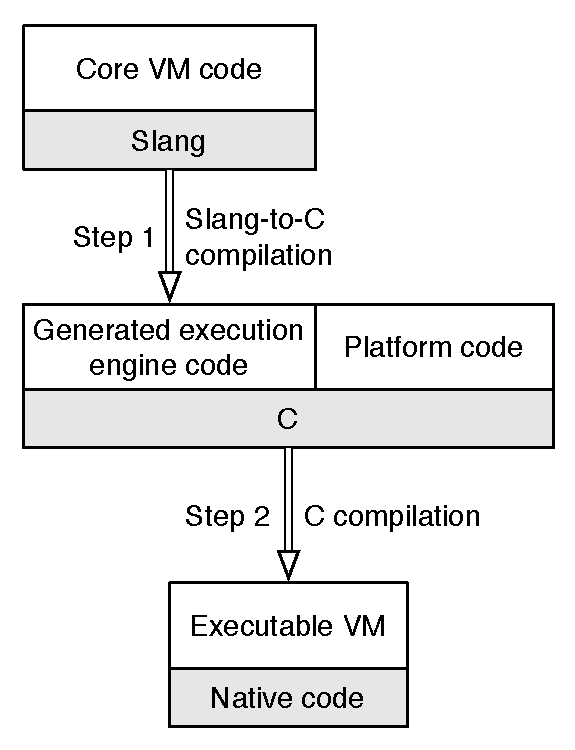
\includegraphics[width=0.45\linewidth]{VMCompilation}
        \caption{VM executable generation}
        \label{fig:VMCompilation}
    \end{center}
\end{figure}

\paragraph{Baseline JIT.}
Cogit is currently used as the baseline JIT. It takes a v-function as input, generates a n-function and installs it. Cogit performs three main kind of optimisations:
\begin{enumerate}
	\item \emph{Stack-to-register mapping:} As the v-functions are encoded using a stack-based bytecode set, values are constantly pushed and popped off the stack. To avoid this behavior, Cogit simulates the stack state during compilation. When reaching an instruction using values on stack, Cogit uses a dynamic template scheme to generate the native instructions. The simulated stack provides information such as which values are constants or already in registers. Based on this information, Cogit picks one of the available template for the instruction, use a linear scan algorithm to allocate registers that do not need to be fixed into specific concrete registers and generate the native instructions.
	\item \emph{Inline caches:} Each virtual call is compiled to an unlinked inline cache. During execution, the inline cache is relinked to a monomorphic, polymorphic or megamorphic inline cache~\cite{Deut84a,Holz91a} when new receiver types are met. The inline caches improve performance but also allows, through n-function introspection, to determine which types were met during previous runs of each virtual call site.
	\item \emph{Calling convention:} Cogit defines specific calling conventions for calls in-between n-functions. Typically, the receiver of the virtual call is always passed by register, and the arguments may or may not be passed by registers depending on how many there are. This is especially efficient to speed-up the inline cache logic and for primitive methods that have an assembly template available as they can directly use the values in registers.
\end{enumerate}

Cogit provides abstractions over the different memory managers supported by the VM (including 32-bits and 64-bits abstractions) and the different assembly back-ends. Most of the optimisations performed are platform-independent, through specific parts, such as inline cache relinking, needs to be implemented differently in each back-end. Cogit currently supports four different back-ends in production: x86, x64, ARMv6 and MIPSEL.

\paragraph{Stack frame reification.}
The current VM evolved from the VM specified in the blue book~\cite{Gold83a}. The original specification relied on a spaghetti stack: the execution stack was represented as a linked list of \emph{contexts}, a context being a v-function activation in the form of an object. Each context was represented as an object that could, as any other object, be read or written by the program. 

Over the years, Deutsch and Schiffman~\cite{Deut84a} changed the VM internal representation of the stack to improve performance. The new stack representation consists of a linked list of stack pages, where each stack page have stack frames next to each other. Most calls and returns, inside a stack page, can use efficient call and return instructions. Only uncommon calls and returns, across stack pages, need to use slower code. With the current production settings, each stack page has enough size to hold around 50 stack frames and different heuristics are used to make calls and returns across stack pages as uncommon as possible. Figure \ref{fig:StackRepresentation} shows the representation of the stack. In the figure, stack pages hold around 5 stack frames to make it easier to read, but in practice stack pages holding less than 40 frames induce considerable overhead.

\begin{figure}[h!]
    \begin{center}
        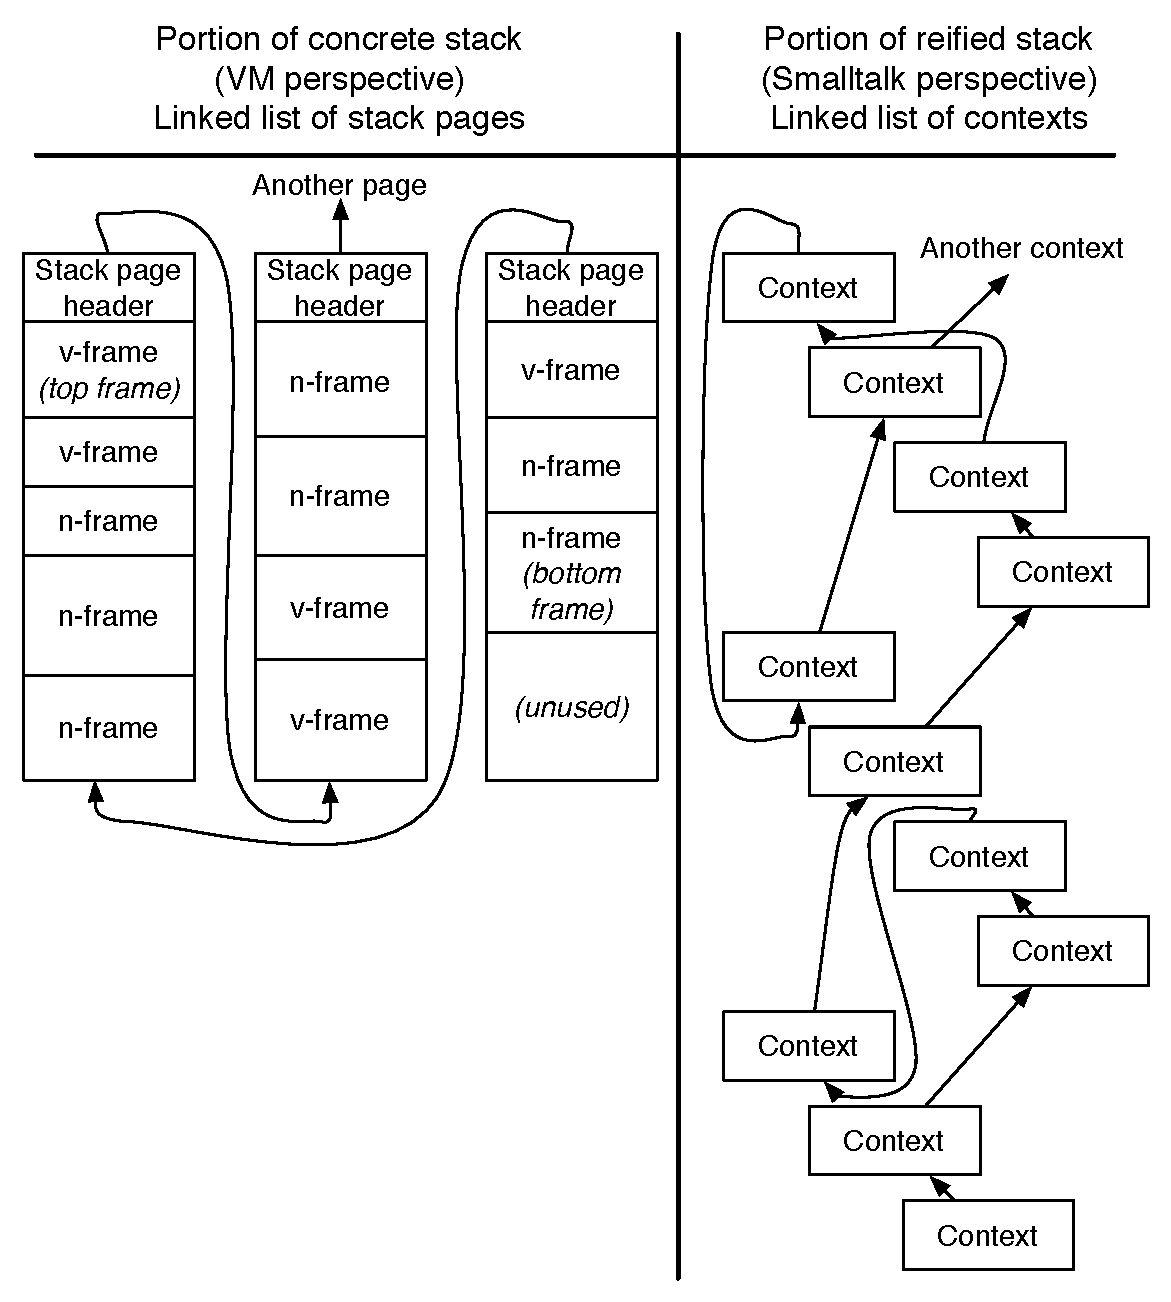
\includegraphics[width=0.52\linewidth]{StackRepresentation}
        \caption{Stack representation}
        \label{fig:StackRepresentation}
    \end{center}
\end{figure}

The VM however still provides the ability for the Smalltalk developer to read and write the reified stack as if it was a linked list of contexts according to the original specification. To do so, the stack is reified as a linked list of contexts on demand. 

The reification of the stack is used in three main places: the debugger, exceptions and continuations. For the two latter, they are implemented in Smalltalk on top of the stack reification, without any special VM support. From Smalltalk, any program can use this feature to instrospect and edit the stack.

Contexts abstract away from low-level details. A context is exactly the same if the VM is started with the interpreter only or with the hybrid interpreter plus baseline JIT runtime. Conceptually, for the Smalltalk developer, the code is interpreted and the contexts always look identical. The VM is responsible to intercept context accesses to read and write concrete v-frames and n-frames.

In the thesis, we will suppose that a context is the same thing as a v-frame as the mapping between both has no impact in the design and brings no interesting additionnal concepts or side-effects. In practice, there are three differences:
\begin{enumerate}
	\item A context is an object while a v-frame use a low-level representation compliant with the stack.
	\item V-frames have to care about some low-level details, such as calls and returns from v-frames to n-frames and n-frames to v-frames, or the access to the v-function arguments by reading values in the caller frame. 
	\item Contexts have a reference to the caller, as conceptually there is a linked list of contexts, while v-frames are below the caller on stack.
\end{enumerate}
However, both v-frames and contexts use the virtual instruction pointer and never the native instruction pointer and both refer to the v-function and never to the n-function. Both representations abstract away from machine-specific state as all the values used by the execution are always on stack and never in registers.

To read and write contexts, the VM intercepts all the accesses to the context objects. To do so, contexts can be in two forms. They can be "married" to a v-frame or n-frame, in which case they act as proxies to the frame. The VM then maps reads and writes to read and write the correct field in the frame representation. Alternatively, they can be "single" (for example when instantiated from Smalltalk), which means there is no stack frame on stack representing the context. In this case, the VM can modify the context as a normal object. Upon activation, the VM lazily recreates a v-frame for a single context to execute it. Returns to single contexts are necessarily across stack page boundaries, hence the overhead to test if the caller is a context on heap or a stack frame on stack is required only in the uncommon case of return across stack pages. 

Aggressive stack manipulation (instruction pointer modification, caller modification) may lead the VM to crash. The program performing such operations needs to guarantee it won't happen, this is not the VM responsibility. In addition, such operations can require a married context to "divorce" the frame, killing the frame in the process. Upon divorce, the stack page is split in two parts and one part if copied to another stack page. One stack page returns to the single divorced context while the context returns to the other stack page, as shown on figure \ref{fig:Divorce}. In normal execution the stack is composed exclusively of stack pages, but after stack manipulation from Smalltalk, the stack can be a linkedlist of stack pages and contexts. 
%as shown on figure \ref{fig:StackRepresentation2}.

\begin{figure}[h!]
    \begin{center}
        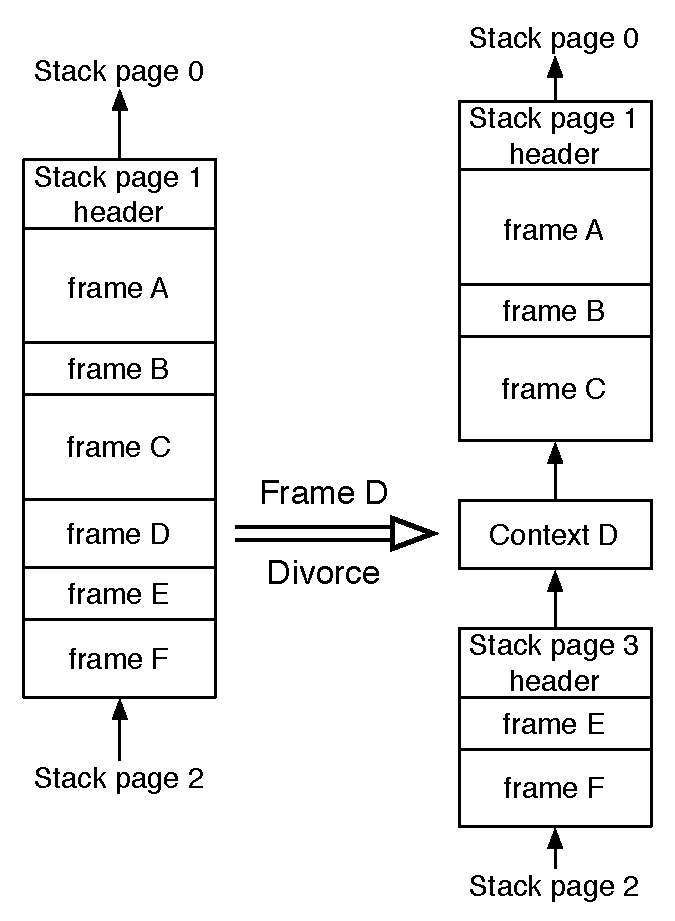
\includegraphics[width=0.55\linewidth]{Divorce}
        \caption{Stack frame divorce}
        \label{fig:Divorce}
    \end{center}
\end{figure}

%\begin{figure}[h!]
%    \begin{center}
%        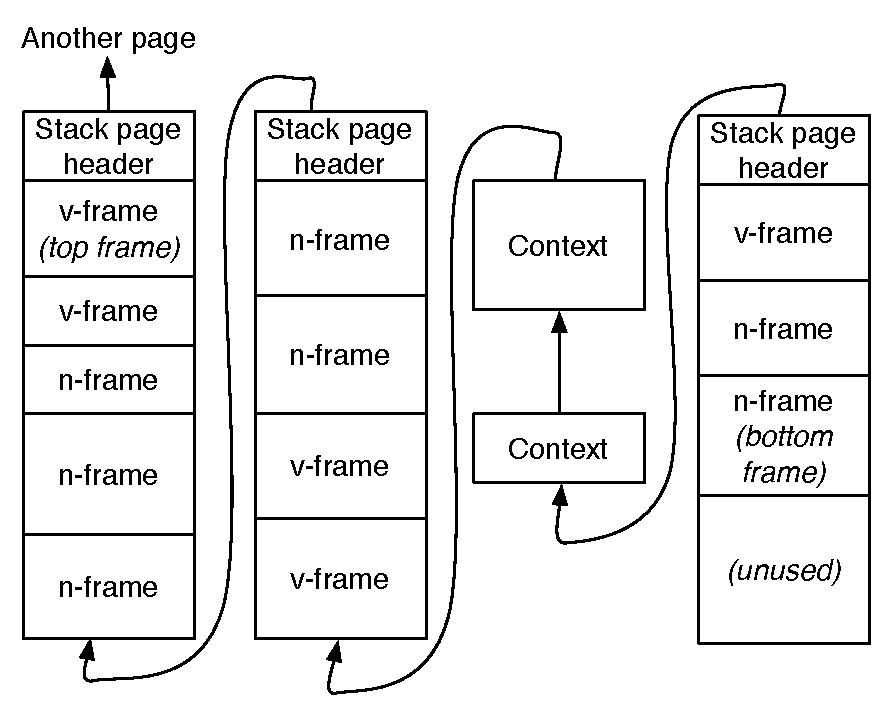
\includegraphics[width=0.7\linewidth]{StackRepresentation2}
%        \caption{Stack representation after stack manipulation}
%        \label{fig:StackRepresentation2}
%    \end{center}
%\end{figure}

Marriage and divorces between stack frames and contexts are not specific to aggressive stack manipulations. They are also used for other features such as snapshots and stack page overflow. In the latter case, as there is a limited number of stack pages (currently 50 in production environments), when a stack page is required and none is available, the VM needs to free a page. To do so, the VM marries then divorces all frames on the least recently used stack page to persist the page in the form of single contexts and re-use the stack page for the execution of new code. 


%%%%%%%%%%%%%%%%%%%%%%%%%%%%%%%%%%%%%%%%%%%%%%%%%%%%%%%%%%%%%%%%%%%%%%%%%%%%%%%%%%%%%%%%%%%%%%%%%%%%%%%%%%%%%%%%%%%%%%%%%%%%%%%

\section{Language-VM interface}

Pharo interfaces with its VM in two different ways:
\begin{enumerate}
	\item Pharo can instantiate v-functions and install them for execution.
	\item A small list of objects is registered in the VM for direct access.
\end{enumerate}

\paragraph{Virtual function representation.}

As everything is an object in Pharo, virtual functions are objects. A v-function is composed of a function's header, a list of literals, a list of bytecodes and a reference to its source code as shown on figure \ref{fig:CompiledCode}. The function's header contains information required for the function's execution such as the number of temporary variables or the size of the frame required.

\begin{figure}[h!]
    \begin{center}
        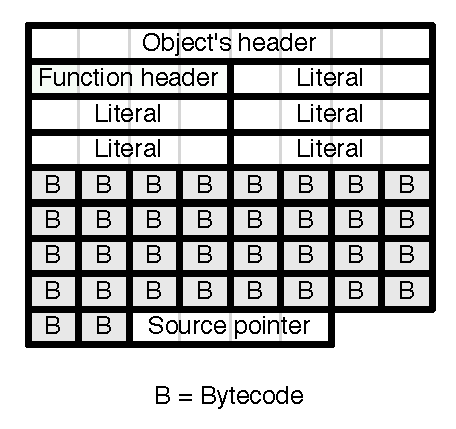
\includegraphics[width=0.38\linewidth]{CompiledCode}
        \caption{Virtual function representation}
        \label{fig:CompiledCode}
    \end{center}
\end{figure}

The bytecode set is stack-based. Most operations are pushing and popping values of the stack. All the operations are untyped and work with any object. One of the main instruction is the virtual call instruction, popping the receiver and arguments from the stack and pushing back the result. The bytecode set also includes conditional and unconditional branches to encode conditions and loops, as well as specific bytecodes to create efficiently closures.


%Move to interface section I believe.

%+ complete list of bytecode instructions, maybe in appendix or a table ? Some of them are duplicated for interpreter performance and compaction (exemple, storePop and push nil), or more or less extended form (uncommon case tke more bytess) but does not really matter.

%Instr - meaning
%In meaning put in emph the variable (index, etc.)

%pushReceiver
%pushLit
%pushThisContext
%pop
%dup
%returnTop
%blockReturnTop

%*2
%pushTemp
%pushInstVar
%pushLitVar
%pushRemoteTemp

%send 
%superSend
%jumpOnTrue
%jumpOnFalse
%jumpForward
%jumpBackward

%createTempVect
%createClosure
%popIntoArray

\subparagraph{Virtual function installation.}

Classes and method dictionaries are normal objects in Pharo. Hence, the installation of a method uses the normal dictionary API, inserting the selector as the key and the method as a value. Method dictionaries, upon modification, request the VM to flush look-up caches for the installed selector. As Pharo is dynamically typed and through uncommon behavior (stack frame modification, exotic primitives) any method can be called by any object, flushing all the methods matching the selector is easier to implement and safer. Closure's functions are installed inside the method that instantiate them as a literal. Changing the literal (hence the closure's function) is normally not done in the current runtime.

\subparagraph{Primitive methods.}

Virtual methods can be annotated with a primitive number at creation time. A primitive method can be executed through a virtual call, like any other method, but upon activation a low-level function (either a Slang function or the native code generated from an assembly code template, depending on the current state of the runtime) is executed. The low-level code can fail if the receiver and arguments of the primitive method do not meet specific constraints. 

Although primitive methods can be used for performance, most of them provides essential features that could not be implemented otherwise. For example, the addition between two integers is implemented as a primitive, forwarding the operation to the processor's implementation of the addition.

Smalltalk features its set of exotic primitives, non present in most other programming languages. A notable example is \ct{become:}, a primitive which swaps the references of two objects. If \ct{a become: b}, then all references to \ct{a} now refer to \ct{b}, and all the references to \ct{b} now refer to \ct{a}. This primitive is implemented efficiently based on specific strategies~\cite{Mir15a}.

\paragraph{Registered objects.} An array of registered objects~\footnote{Smalltalk developers use the term special object array for this array} can be accessed in the Pharo runtime. This array contains multiple objects that need to be accessed directly by the VM, for example the objects \ct{nil, true} and \ct{false}. Any new object can be registered in the array and the array can grow on demand.

Among registered objects are specific selectors. For example, the \ct{\#doesNotUnderstand:} selector is registered. When a look-up performed by the VM does not find any method to activate (the selector is not implemented for the given receiver), the VM instead performs a virtual call, using the same receiver, the registered \ct{\#doesNotUnderstand:} selector and reifies the virtual call as an object (which class is also registered) containing the original selector, the arguments and the look-up class in case of a super send. 

%%%%%%%%%%%%%%%%%%%%%%%%%%%%%%%%%%%%%%%%%%%%%%%%%%%%%%%%%%%%%%%%%%%%%%%%%%%%%%%%%%%%%%%%%%%%%%%%%%%%%%%%%%%%%%%%%%%%%%%%%%%%%%%

\section{Pharo programming language}

This section details two main aspects of the programming language: native thread management and snapshots.

\paragraph{Native threads management.}

Pharo features a global interpreter lock, similarly to python. Only calls to external libraries through the foreign function interface and specific virtual machine extensions have access to the other native threads. Smalltalk execution, including bytecode interpretation, machine code execution, just-in-time compilation and garbage collection are not done concurrently. Being single-threaded has a impact on design decisions because several other VMs implement the optimising JIT in concurrent native threads to the application (CITE Adaptive Optimization in the Jalapeno JVM: The Controller's Analytical Model or maybe somethign with truffle graal).


%TODO, closures and NLR?

\paragraph{Snapshots.}

In the context of Smalltalk, a snapshot~\footnote{Smalltalk developers use the term \emph{image} instead of snapshot.} is a sequence of bytes that represents a serialized form of all the objects present at a precise moment in the runtime. As everything is an object in Smalltalk, including green threads, the virtual machine can, at start-up, load all the objects from a snapshot and resume the execution based on the green thread that was active at snapshot time. In fact, this is the normal way of launching a Smalltalk runtime. 

One interesting problem in snapshots is how to save the execution stack, \ie the green threads. To perform a snapshot, each stack frame is reified into a context and only objects are saved in the snapshot. When the snapshot is restarted, the VM recreates a stack frame for each context lazily. 

In any case, snapshots cannot save n-frames because they are platform-independent. In the Pharo VM for example, a snapshot can be taken on a laptop using a x86 processor and restarted on a raspberry pie using a ARMv6 processor.

%%%%%%%%%%%%%%%%%%%%%%%%%%%%%%%%%%%%%%%%%%%%%%%%%%%%%%%%%%%%%%%%%%%%%%%%%%%%%%%%%%%%%%%%%%%%%%%%%%%%%%%%%%%%%%%%%%%%%%%%%%%%%%%

%Maybe conclusion summary in 1 sentence of chapter + what comes next
\paragraph{Conclusion.} The chapter described the aspects and features of Pharo relevant for the thesis. The following chapter describes the overall Sista architecture.


\ifx\wholebook\relax\else
    \end{document}
\fi
\ifx\wholebook\relax\else

% --------------------------------------------
% Lulu:

    \documentclass[a4paper,12pt,twoside]{../includes/ThesisStyle}

	\usepackage[T1]{fontenc} %%%key to get copy and paste for the code!
%\usepackage[utf8]{inputenc} %%% to support copy and paste with accents for frnehc stuff
\usepackage{times}
\usepackage{ifthen}
\usepackage{xspace}
\usepackage{alltt}
\usepackage{latexsym}
\usepackage{url}            
\usepackage{amssymb}
\usepackage{amsfonts}
\usepackage{amsmath}
\usepackage{stmaryrd}
\usepackage{enumerate}
\usepackage{cite}
%\usepackage[pdftex,colorlinks=true,pdfstartview=FitV,linkcolor=blue,citecolor=blue,urlcolor=blue]{hyperref}
\usepackage{xspace}
%\usepackage{graphicx}
\usepackage{subfigure}
\usepackage[scaled=0.85]{helvet}
        
        
\newcommand{\sepe}{\mbox{>>}}
\newcommand{\pack}[1]{\emph{#1}}
\newcommand{\ozo}{\textsc{oZone}\xspace}
\newcommand\currentissues{\par\smallskip\textbf{Current Issues -- }}

\newboolean{showcomments}
\setboolean{showcomments}{true}
\ifthenelse{\boolean{showcomments}}
  {\newcommand{\bnote}[2]{
	\fbox{\bfseries\sffamily\scriptsize#1}
    {\sf\small$\blacktriangleright$\textit{#2}$\blacktriangleleft$}
    % \marginpar{\fbox{\bfseries\sffamily#1}}
   }
   \newcommand{\cvsversion}{\emph{\scriptsize$-$Id: macros.tex,v 1.1.1.1 2007/02/28 13:43:36 bergel Exp $-$}}
  }
  {\newcommand{\bnote}[2]{}
   \newcommand{\cvsversion}{}
  } 


\newcommand{\here}{\bnote{***}{CONTINUE HERE}}
\newcommand{\nb}[1]{\bnote{NB}{#1}}
\newcommand{\fix}[1]{\bnote{FIX}{#1}}
%%%% add your own macros 

\newcommand{\sd}[1]{\bnote{Stef}{#1}}
\newcommand{\ja}[1]{\bnote{Jannik}{#1}}
\newcommand{\na}[1]{\bnote{Nico}{#1}}
%%% 


\newcommand{\figref}[1]{Figure~\ref{fig:#1}}
\newcommand{\figlabel}[1]{\label{fig:#1}}
\newcommand{\tabref}[1]{Table~\ref{tab:#1}}
\newcommand{\layout}[1]{#1}
\newcommand{\commented}[1]{}
\newcommand{\secref}[1]{Section \ref{sec:#1}}
\newcommand{\seclabel}[1]{\label{sec:#1}}

%\newcommand{\ct}[1]{\textsf{#1}}
\newcommand{\stCode}[1]{\textsf{#1}}
\newcommand{\stMethod}[1]{\textsf{#1}}
\newcommand{\sep}{\texttt{>>}\xspace}
\newcommand{\stAssoc}{\texttt{->}\xspace}

\newcommand{\stBar}{$\mid$}
\newcommand{\stSelector}{$\gg$}
\newcommand{\ret}{\^{}}
\newcommand{\msup}{$>$}
%\newcommand{\ret}{$\uparrow$\xspace}

\newcommand{\myparagraph}[1]{\noindent\textbf{#1.}}
\newcommand{\eg}{\emph{e.g.,}\xspace}
\newcommand{\ie}{\emph{i.e.,}\xspace}
\newcommand{\ct}[1]{{\textsf{#1}}\xspace}


\newenvironment{code}
    {\begin{alltt}\sffamily}
    {\end{alltt}\normalsize}

\newcommand{\defaultScale}{0.55}
\newcommand{\pic}[3]{
   \begin{figure}[h]
   \begin{center}
   \includegraphics[scale=\defaultScale]{#1}
   \caption{#2}
   \label{#3}
   \end{center}
   \end{figure}
}

\newcommand{\twocolumnpic}[3]{
   \begin{figure*}[!ht]
   \begin{center}
   \includegraphics[scale=\defaultScale]{#1}
   \caption{#2}
   \label{#3}
   \end{center}
   \end{figure*}}

\newcommand{\infe}{$<$}
\newcommand{\supe}{$\rightarrow$\xspace}
\newcommand{\di}{$\gg$\xspace}
\newcommand{\adhoc}{\textit{ad-hoc}\xspace}

\usepackage{url}            
\makeatletter
\def\url@leostyle{%
  \@ifundefined{selectfont}{\def\UrlFont{\sf}}{\def\UrlFont{\small\sffamily}}}
\makeatother
% Now actually use the newly defined style.
\urlstyle{leo}



	\usepackage{amsmath,amssymb}             % AMS Math
% \usepackage[french]{babel}
\usepackage[latin1]{inputenc}
\usepackage[T1]{fontenc}
\usepackage[left=1.5in,right=1.3in,top=1.1in,bottom=1.1in,includefoot,includehead,headheight=13.6pt]{geometry}
\renewcommand{\baselinestretch}{1.05}

\usepackage{multicol}

% Table of contents for each chapter

\usepackage[nottoc, notlof, notlot]{tocbibind}
\usepackage{minitoc}
\setcounter{minitocdepth}{1}
\mtcindent=15pt
% Use \minitoc where to put a table of contents

\usepackage{enumitem}

\usepackage{aecompl}

% Glossary / list of abbreviations

%\usepackage[intoc]{nomencl}
%\renewcommand{\nomname}{List of Abbreviations}
%
%\makenomenclature

% My pdf code

\usepackage[pdftex]{graphicx}
\usepackage[a4paper,pagebackref,hyperindex=true]{hyperref}

\usepackage{pgfplotstable,booktabs,colortbl}
\pgfplotsset{compat=1.8}

% Links in pdf
\usepackage{color}
\definecolor{linkcol}{rgb}{0,0,0.4} 
\definecolor{citecol}{rgb}{0.5,0,0} 

% Change this to change the informations included in the pdf file

% See hyperref documentation for information on those parameters

\hypersetup
{
bookmarksopen=true,
pdftitle="Sista: a Metacircular Architecture for Runtime Optimisation Persistence",
pdfauthor="Clement BERA", 
pdfsubject="Thesis", %subject of the document
%pdftoolbar=false, % toolbar hidden
pdfmenubar=true, %menubar shown
pdfhighlight=/O, %effect of clicking on a link
colorlinks=true, %couleurs sur les liens hypertextes
pdfpagemode=None, %aucun mode de page
pdfpagelayout=SinglePage, %ouverture en simple page
pdffitwindow=true, %pages ouvertes entierement dans toute la fenetre
linkcolor=linkcol, %couleur des liens hypertextes internes
citecolor=citecol, %couleur des liens pour les citations
urlcolor=linkcol %couleur des liens pour les url
}

% definitions.
% -------------------

\setcounter{secnumdepth}{3}
\setcounter{tocdepth}{1}

% Some useful commands and shortcut for maths:  partial derivative and stuff

\newcommand{\pd}[2]{\frac{\partial #1}{\partial #2}}
\def\abs{\operatorname{abs}}
\def\argmax{\operatornamewithlimits{arg\,max}}
\def\argmin{\operatornamewithlimits{arg\,min}}
\def\diag{\operatorname{Diag}}
\newcommand{\eqRef}[1]{(\ref{#1})}

\usepackage{rotating}                    % Sideways of figures & tables
%\usepackage{bibunits}
%\usepackage[sectionbib]{chapterbib}          % Cross-reference package (Natural BiB)
%\usepackage{natbib}                  % Put References at the end of each chapter
                                         % Do not put 'sectionbib' option here.
                                         % Sectionbib option in 'natbib' will do.
\usepackage{fancyhdr}                    % Fancy Header and Footer

% \usepackage{txfonts}                     % Public Times New Roman text & math font
  
%%% Fancy Header %%%%%%%%%%%%%%%%%%%%%%%%%%%%%%%%%%%%%%%%%%%%%%%%%%%%%%%%%%%%%%%%%%
% Fancy Header Style Options

\pagestyle{fancy}                       % Sets fancy header and footer
\fancyfoot{}                            % Delete current footer settings

%\renewcommand{\chaptermark}[1]{         % Lower Case Chapter marker style
%  \markboth{\chaptername\ \thechapter.\ #1}}{}} %

%\renewcommand{\sectionmark}[1]{         % Lower case Section marker style
%  \markright{\thesection.\ #1}}         %

\fancyhead[LE,RO]{\bfseries\thepage}    % Page number (boldface) in left on even
% pages and right on odd pages
\fancyhead[RE]{\bfseries\nouppercase{\leftmark}}      % Chapter in the right on even pages
\fancyhead[LO]{\bfseries\nouppercase{\rightmark}}     % Section in the left on odd pages

\let\headruleORIG\headrule
\renewcommand{\headrule}{\color{black} \headruleORIG}
\renewcommand{\headrulewidth}{1.0pt}
\usepackage{colortbl}
\arrayrulecolor{black}

\fancypagestyle{plain}{
  \fancyhead{}
  \fancyfoot{}
  \renewcommand{\headrulewidth}{0pt}
}

\usepackage{algorithm}
\usepackage[noend]{algorithmic}

%%% Clear Header %%%%%%%%%%%%%%%%%%%%%%%%%%%%%%%%%%%%%%%%%%%%%%%%%%%%%%%%%%%%%%%%%%
% Clear Header Style on the Last Empty Odd pages
\makeatletter

\def\cleardoublepage{\clearpage\if@twoside \ifodd\c@page\else%
  \hbox{}%
  \thispagestyle{empty}%              % Empty header styles
  \newpage%
  \if@twocolumn\hbox{}\newpage\fi\fi\fi}

\makeatother
 
%%%%%%%%%%%%%%%%%%%%%%%%%%%%%%%%%%%%%%%%%%%%%%%%%%%%%%%%%%%%%%%%%%%%%%%%%%%%%%% 
% Prints your review date and 'Draft Version' (From Josullvn, CS, CMU)
\newcommand{\reviewtimetoday}[2]{\special{!userdict begin
    /bop-hook{gsave 20 710 translate 45 rotate 0.8 setgray
      /Times-Roman findfont 12 scalefont setfont 0 0   moveto (#1) show
      0 -12 moveto (#2) show grestore}def end}}
% You can turn on or off this option.
% \reviewtimetoday{\today}{Draft Version}
%%%%%%%%%%%%%%%%%%%%%%%%%%%%%%%%%%%%%%%%%%%%%%%%%%%%%%%%%%%%%%%%%%%%%%%%%%%%%%% 

\newenvironment{maxime}[1]
{
\vspace*{0cm}
\hfill
\begin{minipage}{0.5\textwidth}%
%\rule[0.5ex]{\textwidth}{0.1mm}\\%
\hrulefill $\:$ {\bf #1}\\
%\vspace*{-0.25cm}
\it 
}%
{%

\hrulefill
\vspace*{0.5cm}%
\end{minipage}
}

\let\minitocORIG\minitoc
\renewcommand{\minitoc}{\minitocORIG \vspace{1.5em}}

\usepackage{multirow}
\usepackage{slashbox}

\newenvironment{bulletList}%
{ \begin{list}%
	{$\bullet$}%
	{\setlength{\labelwidth}{25pt}%
	 \setlength{\leftmargin}{30pt}%
	 \setlength{\itemsep}{\parsep}}}%
{ \end{list} }

\newtheorem{definition}{D�finition}
\renewcommand{\epsilon}{\varepsilon}

% centered page environment

\newenvironment{vcenterpage}
{\newpage\vspace*{\fill}\thispagestyle{empty}\renewcommand{\headrulewidth}{0pt}}
{\vspace*{\fill}}



	\graphicspath{{.}{../figures/}}
	\begin{document}
\fi

\chapter{Sista Architecture}
\label{chap:architecture}
\minitoc

%Generic intro + overview intro
The overall thesis focuses on the design and implementation of an optimising JIT compiler for Pharo, written in Pharo itself, running in the same runtime than the optimised application on top of the existing runtime environment. The chapter explains the overall architecture designed and implemented, called the Sista architecture. The first section gives an overview of the architecture. Section \ref{sec:functionOptimisation} details how functions are optimised. Section \ref{sec:functionDeoptimisation} focuses on the deoptimisation of optimised stack frames when an assumption taken at optimisation time is not valid at runtime. Section \ref{sec:relatedWorkArch} compares the Sista architecture against related work.

%%%%%%%%%%%%%%%%%%%%%%%%%%%%%%%%%%%%%%%%%%%%%%%%%%%%%%%%%%%%%%%%%%%%%%%%%%%%%%%%%%%%%%%%%%%%%%%%%%%%%%%%%%%%%%%%%%%%%%%%

\section{Overview}

This section starts by describing briefly the existing runtime and evolutions required to introduce an optimising JIT. Section \ref{sec:splitDesign} explain the overall design. As the architecture is different from classical architectures, the terminology is clarified in section \ref{sec:terminologyI}. Lastly, section \ref{sec:further} briefly describe how functions are optimised and deoptimised. 

\subsection{Existing runtime}

The existing Pharo runtime relies on a v-function interpreter and a baseline JIT named Cogit to execute functions. Cogit is able to compile a single v-function to a single n-function with a limited number of optimisations such as inline caches~\cite{Deut84a,Holz91a}. Cogit does not perform optimisations requiring speculations based on runtime information. To load new code in Smalltalk, it is possible to install new v-functions at runtime. In this case, the program requests the VM to flush caches matching the new v-functions installed.

Compared to the function based architecture described in the previous chapter, the Pharo runtime is missing entirely an optimising JIT performing speculative optimisations based on runtime information. The first missing feature is that the baseline JIT is not able to detect hotspots to trigger the optimising JIT nor to introspect the n-function it generates to provide runtime information. The second missing feature is the optimising JIT itelf, which should be able to generate an optimised n-function from v-functions and the corresponding runtime information. The optimising JIT needs to include specific components in addition to the optimisation pipeline. A deoptimiser is needed to resume execution with non optimised code when a speculation made at optimisation time is incorrect at runtime. A dependency manager is required to discard dependant optimised functions when new code is loaded.

\subsection{Split design}
\label{sec:splitDesign}

The architecture requires both baseline JIT extensions and the addition of the optimising JIT.

\paragraph{Baseline JIT extensions.}
The existing baseline JIT, Cogit, had to be extended to detect hot spots and to provide runtime information to direct the optimising JIT decisions. 

To detect hot spots, Cogit was extended to be able to generate profiling counters in generated n-functions. When a profiling counter reaches a specific threshold, a specific routine is triggered and may activate an optimising JIT. More details on the profiling counters are present in section \ref{sec:hotSpot}.

Cogit was already able to introspect the n-function it generates for multiple purposes, such as debugging, inline cache relinking or literals garbage collection. The introspection logic was extended to provide a new primitive method in Smalltalk, which answers for a given function both the values present in inline caches and the values of profiling counters.

\paragraph{Optimising JIT.}
The optimising JIT was designed in two different parts as shown in figure \ref{fig:OptArchitecture}. The high-level part is a non optimised v-functions to optimised v-function compiler called \emph{Scorch}. The second part is a v-function to a n-function compiler and an extended version of Cogit, the baseline JIT, is used. The compilation of non optimised v-functions to an optimised n-function through Scorch followed by Cogit forms an optimising JIT.

Scorch is written in Pharo and runs in the same runtime as the optimised application in a metacircular style. Scorch deals with Smalltalk-specific optimisations. Hence, any work performed on Scorch is done in Smalltalk dealing with Smalltalk-specific optimisations. Such work can be performed with little knowledge on low-level or machine-specific details. The optimised v-functions generated by Scorch may use unsafe instructions in addition to the non optimised v-function instructions. Unsafe instructions are faster to execute but requires the compiler to guarantee specific invariants.

\begin{figure}[h!]
    \begin{center}
        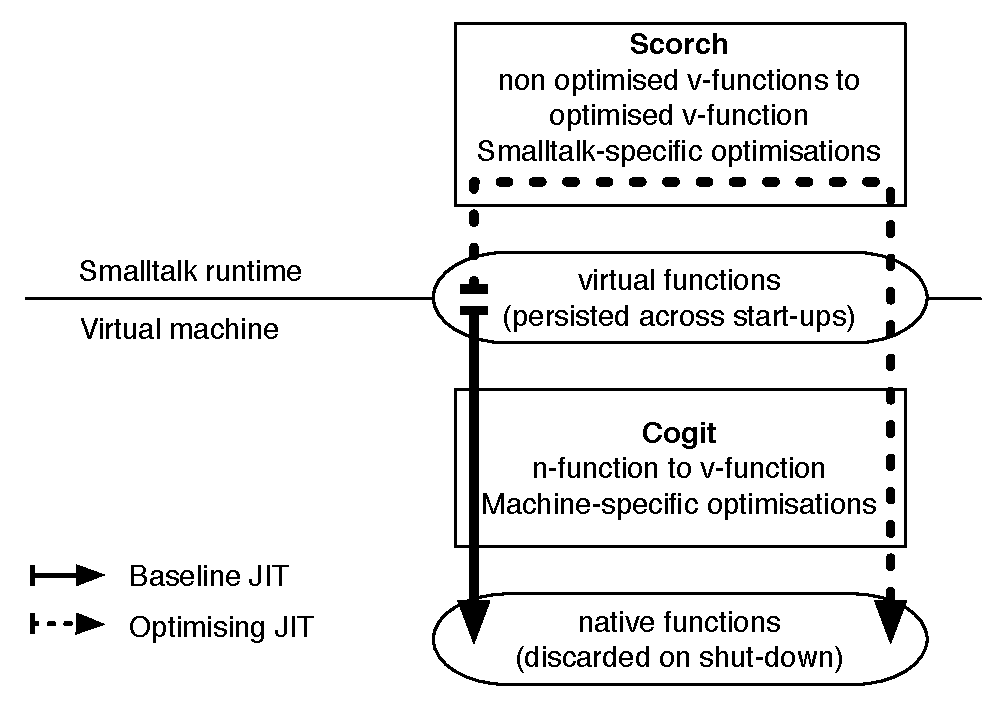
\includegraphics[width=0.8\linewidth]{OptArchitecture}
        \caption{Scorch critical and background modes}
        \label{fig:OptArchitecture}
    \end{center}
\end{figure}

For the low-level part, the existing baseline JIT Cogit is reused. Cogit may perform machine-specific optimisations. To be used as a back-end for the optimised v-functions, Cogit was extended to support the new unsafe instructions, including a specific VM call-back to trigger deoptimisation when an assumption speculated at optimisation time is invalid at runtime.

\subsection{Terminology}
\label{sec:terminologyI}
\emph{Sista} is the named of the overall architecture detailled in the thesis. As the architecture has notable differences from the standard tiered architecture, the two runtime compilers are not really a baseline JIT and an optimising JIT. We call them by their project name in the thesis. The first runtime compiler is called \emph{Scorch} and compiles v-functions to optimised v-functions using speculative optimisations. Scorch is written in plain Smalltalk. The second runtime compiler is called \emph{Cogit} and compiles v-functions to n-functions. Cogit can be used alone as the baseline JIT, or as a back-end for Scorch. In the later case, the pair of Scorch and Cogit forms an optimising JIT. Cogit is written in a restrictive Smalltalk compiled ahead-of-time to an executable as part of the VM. 

In this context, both v-functions and n-functions can have an optimised version. We therefore used the term v-function to discuss all v-functions (optimised or not), and specify optimised v-function and non optimised v-function when needed. Similarly, for frames, we say v-frame to discuss v-frames in general, and specify optimised v-frame and non optimised v-frame when discussing a v-frame respectively representing the execution state of an optimised v-function or a non optimised v-function. The same terminology is used with native (\emph{n-}) than with virtual (\emph{v-}).

Both runtime compilers can deoptimise stack frames. Cogit can deoptimise any n-frame to a single v-frame. 
%Cogit also provides proxies to introspect a n-frame as a v-frame, though certain operations such as instruction pointer mutation do not work with proxies but require deoptimisation from a n-frame to a v-frame. 
Scorch can deoptimise an optimised v-frame to multiple non optimised v-frames. 

\subsection{Optimisation and deoptimisation}
\label{sec:further}

%opt intro
Cogit was extended to detect hot spot through profiling counters in non optimised n-functions. When a hot spot is detected, Cogit immediately calls Scorch in Pharo. Scorch then looks for the best v-function to optimise based on the current stack, optimises it and installs the optimised version. To perform optimisation, Scorch may ask Cogit to introspect specific n-functions to extract type information and basic block usage from previous runs. Once installed, the VM can execute the optimised v-function at the next call to the function. As the VM runtime is hybrid between the interpreter and Cogit, the optimised v-function may conceptually be interpreted or compiled by Cogit and then executed as an optimised n-function. In practice, new heuristics were introduced for optimised v-functions to execute them as optimised n-functions from the first run. The details of the function optimisation logic is written in section \ref{sec:functionOptimisation}.

%deopt intro
Due to speculative optimisations, optimised v-functions may contain guards to ensure optimisation-time assumptions are valid at runtime. If a guard fails, the execution stack needs to be deoptimised to resume execution with non optimised code. When an optimised n-frame needs to be deoptimised, Cogit maps the optimised n-frame to a single optimised v-frame. Cogit then provides the optimised v-frame to Scorch, which maps the optimised v-frame to multiple non optimised v-frames. Scorch may discard the optimised v-function if guards are failing too often in it. The execution can then resume using non optimised v-functions. The deoptimisation logic briefly described here is explained in detail in section \ref{sec:functionDeoptimisation}.

%%%%%%%%%%%%%%%%%%%%%%%%%%%%%%%%%%%%%%%%%%%%%%%%%%%%%%%%%%%%%%%%%%%%%%%%%%%%%%%%%%%%%%%%%%%%%%%%%%%%%%%%%%%%%%%%%%%%%%%%

\section{Function optimisation}
\label{sec:functionOptimisation}

%Intro
Cogit was extended to detect hot spots based on profiling counters. When a hot spot is detected, Cogit triggers a call-back to request Scorch to optimise a v-function based on the current stack. As Pharo is currently single-threaded, the application green thread has to be interrupted to optimise a function. The overall design is then the following: after interrupting the application, Scorch finds a v-function to optimise based on the current stack, optimises it, installs the optimised version, and resumes the application. The optimised v-function installed will be executed at the next call of the function.

\subsection{Optimiser critical and background modes}

%TimeBeforePostPoning: problem so it's required
Scorch's optimiser may however require a significant amount of time to optimise a v-function. Optimising a v-function can take a long time in slow machines or when a pathological function~\footnote{Many compiler algorithms have a good average complexity based on heurisitics but poor worst complexity. A pathological function is a function not matching any heuristic leading to long optimisation time.} is optimised. This can lead to an interruption of the application for an amount time long enough to be noticed by the user. To experiment with the Sista architecture, we worked with the development environment of Pharo (which is written in Pharo). In the case of a user-interface application like this one, it is \emph{very} annoying to see the application interrupted during half a second or more when multiple v-functions long to optimise are optimised in a row. The user interface feels slow, lagging and unresponsive even though the overall code takes less time to execute.

%First solution: timeBeforePostponing, with constraint for long methods
To avoid the problem, we limited the optimisation time to a fixed small time period, configured from the language. For user interface application, we limit it to 40 ms. The limitation is enforced by a high-priority green thread, set to stop the optimiser after the given time period. As the current user interface is refreshing at 50Hz, the optimiser, in the worst case, force the system not to refresh the screen twice. In practice, most v-functions are optimised in less than 40ms. However, some v-functions are still too long to optimise, so an alternative solution is required to optimise them.
%Didn't use frame before not to confuse graphic frames with stack frames.

%idle and postpone
Upon profiling the development tools, as one would expect, we noticed that the application spends a significant amount of time in idle\footnote{An application in idle means it has nothing to do, it is typically waiting for an event to do anything.}. We show for example in figure \ref{fig:ApplicationIdle} that the application is successfully executing code, then idle, then executing code again, etc. In this case, each time an event happen (key stroke, mouse click, etc.), some code is executed, but when no event happens, for example when the developer is reading code, the application is in idle.

\begin{figure}[h!]
    \begin{center}
        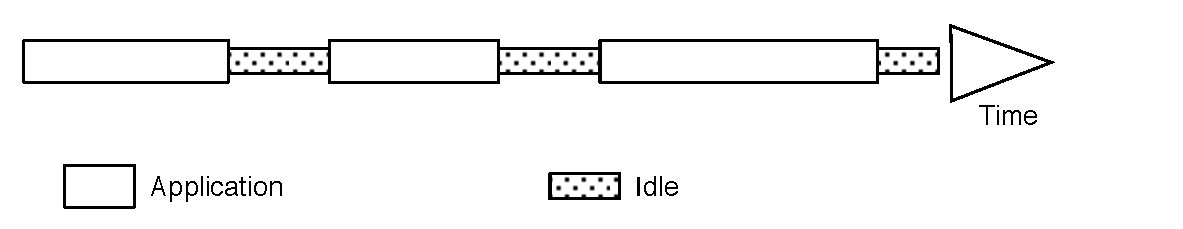
\includegraphics[width=0.95\linewidth]{ApplicationIdle}
        \caption{User interface application idle times}
        \label{fig:ApplicationIdle}
    \end{center}
\end{figure}

%background thread
Based on the profiling result, we introduced a background green thread responsible for optimising the functions too long to optimise in the limited time period allowed. This way, when the application would normally become idle, it starts by optimising such functions and becomes idle when no functions to optimise are remaining. As the background green thread is running at low priority, if the application restarts while an optimisation is being performed, the application green thread preempts the optimisation green thread and no pauses are seen by the user.

%Critical vs background
The optimiser can therefore be run in two mode. When a hot spot is detected, the optimiser is started in \emph{critical mode}. It has a limited time period to optimise a function based on the current stack. If the optimisation takes too long, the function to optimise is added to the background compilation queue. When the application becomes idle, if the background compilation queue is not empty, the optimiser is started in \emph{background mode}. In background mode, the optimiser is run in a low-priority green thread and is preempted by any application green thread. When the optimiser has optimised all the functions in the compilation queue, it stops and the application becomes idle. Scorch's optimiser critical and background modes are represented on figure \ref{fig:ScorchModes}.

\begin{figure}[h!]
    \begin{center}
        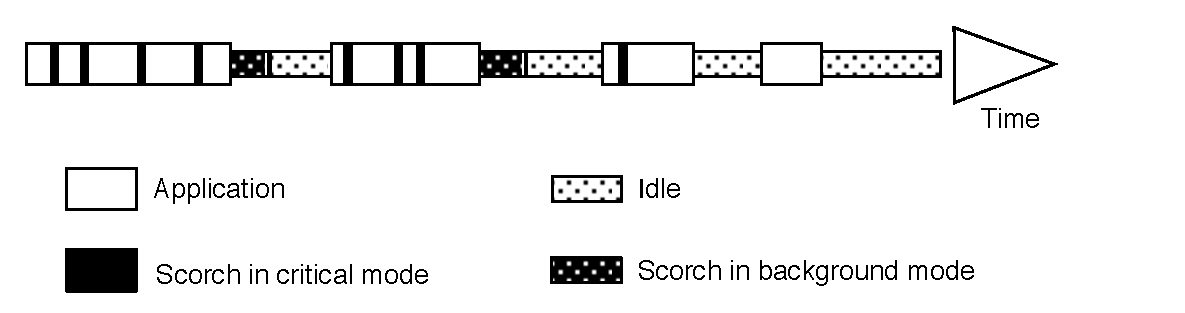
\includegraphics[width=0.95\linewidth]{ScorchModes}
        \caption{Scorch critical and background modes}
        \label{fig:ScorchModes}
    \end{center}
\end{figure}

%Merged with previous paragraph.  Fig explanation, critical vs background mode
%As shown on figure \ref{fig:ScorchModes}, when the application is running, it can be interrupted for a small time window at worst. When the application normally becomes idle, the background green thread starts optimising the functions long to optimise. When no more functions are queued for optimisations, the application becomes idle. In any case, after a while, all critical portions of code have been optimised and the application is usually not interrupted any more while the background green thread has usually no more v-functions to optimise.

\paragraph{Conclusion.}The Scorch optimiser can be run in two modes. In critical mode, it interrupts the application green thread and has a limited time period to optimise a function. If the time limit is not enough, the function's optimisation is postponed to the background mode. In background mode, Scorch optimises code only when the application is idle but has no time limit. This design allow all the application's code to be optimised in a single-threaded environment without the system loosing too much responsiveness.

\subsection{Hot spot management}
\label{sec:hotSpot}

%generic profiling counters
Cogit was extended to be able to generate n-functions with profiling counters. Profiling counters allow to detect hot spots and provide information about basic block usage at the cost of a small overhead, detailled in the validation chapter of the thesis. Because of the overhead, Cogit was extended to support conditionnal compilation. Based on a specific bit in the v-function's header, Cogit compiles the v-function with or without profiling counters. Typically, non optimised v-functions, produced by the source code to v-function bytecode compiler~\cite{Bera13a}, are by default compiled to n-functions with profiling counters, while optimised v-functions are compiled without profiling counters. Profiling counters are generated so that the counter is increased by one when the execution flow reaches it and a specific hot spot detection routine is called when the counter reaches a threshold.

%SHOW v-function header format ?

%Counters on branch
Based on \cite{Arn02}, we added counters by extending the way the baseline JIT generates conditional jumps. Counters are added just before and just after the branch. In several other VMs, the counters are added at the beginning of each function. The technique we used allowed us to reduce the counter overhead as branches are 6 times less frequent that virtual calls in Smalltalk. In addition, the counters provide information about basic block usage. Every finite loop requires a branch to stop the loop iteration and most recursive code requires a branch to stop the recursion, so the main cases where hot spots are present are detected.

%hot spot detection - call-back
When a hot spot is detected, a specific Slang routine is called. The routine makes sure the n-frame where the hot spot is detected is reified so it can be introspected from Smalltalk. Then, the routine performs a virtual call with a selector registered from Smalltalk, the reified stack frame as the receiver and the boolean the conditionnal jump was branching on as a parameter. The method activated by the call-back, in Smalltalk, calls the Scorch optimiser.

During optimisation, the bottom frames of the execution stack are used by the Scorch optimiser. The frame above is the call-back frame, followed by the application frame holding the n-function with the hot spot, as shown on figure \ref{fig:HotSpotCallBackStack}.

\begin{figure}[h!]
    \begin{center}
        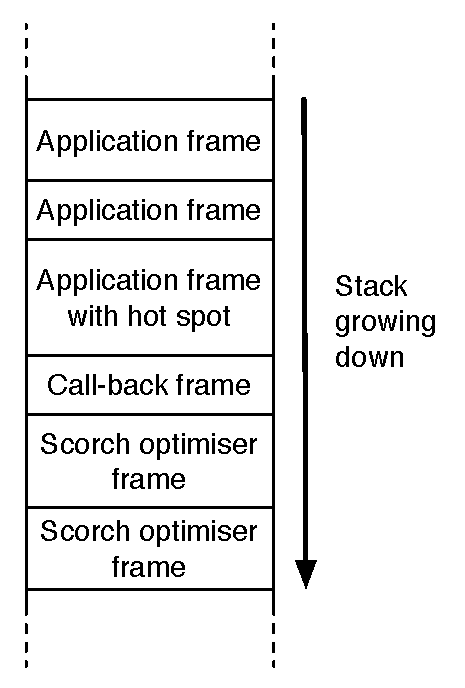
\includegraphics[width=0.35\linewidth]{HotSpotCallBackStack}
        \caption{Stack state during critical mode optimisation}
        \label{fig:HotSpotCallBackStack}
    \end{center}
\end{figure}

%Flag: FRAMEREIFICATION.

%returning from call-back
The profiling counter machine code is generated so that upon return to the n-frame with the profiling counter, the conditionnal branch is performed again on the value returned. This way, if the Smalltalk code resets the profiling counters and returns the boolean passed by argument to the call-back, the application execution is resumed by performing one more time the branch with the same boolean.

%WARNING ! What happen when conditionalBranchTrip and reification.

\subsection{Scorch optimiser}

The Scorch optimiser is activated by the call-back and has access to the reified stack. Scorch firstly analyse the stack and finds the best function to optimise. Then, it generates, either directly in critical mode or indirectly through background mode an optimised v-function and installs it for further uses.

%TO REMOVE
%We call the \emph{tripping function} the function where the hot spot is detected, because a counter has "tripped" in this function.

\paragraph{Stack search.}
\label{ss:stackSearch}

%Function selection, bottom is bad
When a hot spot is detected, Scorch is activated and has access to the reified stack. A naive approach would be to always optimise the function where the hot spot is detected and not to search the stack at all. Unfortunately, this heuristic would be terrible for Smalltalk. An important part of the execution time is due to the extensive use of closures. More specifically, most loops in the executed code, assuming the code respects standard Smalltalk coding conventions, are using closures. To efficiently remove the closure overhead, the closure needs to be inlined up to its enclosing environment to remove both the closure creation and the closure activation. If the function where the hot spot is detected is either activating closures or a closure activation itself, then optimising it won't gain that much performance because the closure creation and activation execution time will remain.

%Function selection, bottom or home is bad
Another approach, a bit less naive, would be to optimise the function where the hot spot is detected if it is a method, and the enclosing environment's function if it is a closure, in an attempt to remove closure overhead. Yet, this heuristic still does not solve the most common case of the problem. To illustrate the problem, let's look at a simple example with a loop over an array.

%array loop example. descr exampleArrayLoop
In the code sample in figure \ref{fig:ExampleCode}, \ct{exampleArrayLoop} is a method installed in the class \ct{ApplicationClass}. Its method body consists of a loop over an array, the array being an instance variable. To loop over an array, Smalltalk provides high level construct such as \ct{do:}. In this case, \ct{do:} is very similar to \ct{foreach} in other languages and allows to iterate over the array while providing at each iteration of the loop the array's element in the variable \ct{element}. The \ct{do:} method, installed in \ct{Array}, takes a single argument, a closure, which is evaluated using \ct{value:} at each iteration of the loop. The parameter of the closure activation is \ct{self at: i}, which represent the access to the element \ct{i} of the array. During the closure evaluation, the bottom three frames are the closure activation, the frame for \ct{Array >> do:} and the frame for \ct{ApplicationClass >> exampleArrayLoop} as shown on figure \ref{fig:ExampleLoopStack}.

\begin{figure}[h!]
    \begin{center}
        \begin{code}
        	ApplicationClass >> exampleArrayLoop
        	    array do: [ :element | FileStream stdout nextPutAll: element printString ].
        		
        	Array >> do: aClosure
        	    1 to: self size do: [:index | aClosure value: (self at: index)].
        \end{code}   
	\caption{Example code}
        \label{fig:ExampleCode}
    \end{center}
\end{figure}

\begin{figure}[h!]
    \begin{center}
        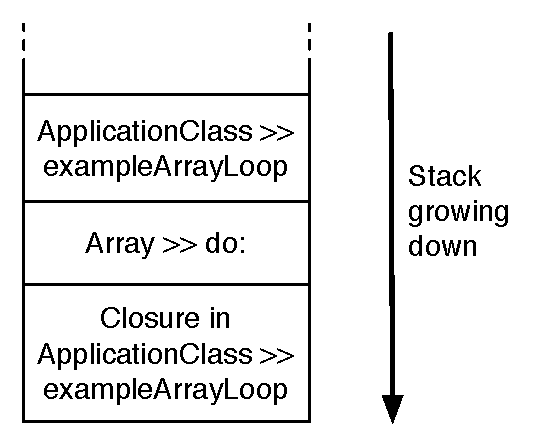
\includegraphics[width=0.42\linewidth]{ExampleLoopStack}
        \caption{Example stack during closure execution}
        \label{fig:ExampleLoopStack}
    \end{center}
\end{figure}

%descr do:
The method \ct{Array >> do:} is using a special selector, \ct{to:do:}, which is compiled by the bytecode compiler to a loop, in a similar way to \ct{for} constructs in other programming languages. In fact, the \ct{Array >> do:} method body is a loop from 1 to the size of the array, evaluating the closure at each iteration for each element in the array. At each iteration, the current value of index is tested against the size of the array, and when that value is reached the loop is exited.

%profiling counter location
As discussed in the previous section, profiling counters detect frequent portion of code on branches. Each finite loop has a branch to either keep iterating over the loop or exit the loop. In the example, it means that the method \ct{Array >> do:} has a profiling counter on the branch testing the value of the index against the size of the array. The rest of the code, in the two methods and in the closure, have no other profiling counters.

%closure issue and why to pick next function
The hot spot is going to be detected on the profiling counter, hence in the method \ct{Array>>do:}. If Scorch optimised the \ct{Array>>do:} method, it cannot know what closure will be executed as the closure is an argument, while an important part of the execution time is spent creating and evaluating the closure. However, if \ct{Array>>do:} gets inlined into \ct{ApplicationClass>>exampleArrayLoop}, the closure evaluated would be known to be the closure \ct{[ :element | FileStream stdout nextPutAll: element printString ]}. Hence, to gain maximum performance, the optimiser should decide to optimise \ct{ApplicationClass>>exampleArrayLoop} and inline both the \ct{Array>>do:} method and the closure evaluation (\ct{value:}). 

%detail of the problem
In this case, the hot spot is detected in \ct{Array>>do:}. The hot spot is therefore detected in a method, not a closure. Naive heuritics would have chosen to optimise \ct{Array>>do:}, while it is better to select the caller stack frame's function.

%closure last explanation
Overall, because of the extensive use of closures, the optimiser almost never chose to optimiser the function where the hot spot is detected. It usually walks up a few frames to find the best function to optimise. 

\paragraph{Optimised v-function generation.}
Once Scorch has selected the v-function to optimise, it generates an optimised v-function. It attempts to do it immediately, within a limited amount of time. If it fails to do it, it postpones the optimisation to background mode. The function's optimisation and installation is using the same code in both cases, so we will discuss only the critical mode optimisation in the following paragraphs.

Scorch's optimiser is implemented with traditional compiler optimisation techniques. It decompiles the v-function to optimise into a single static assignment intermediate representation, represented in the form of a control flow graph. Specific instructions that may require deoptimisation of the optimised frame have deoptimisation metadata attached which is updated during the optimisation passes to still refer to the correct values. During decompilation, Scorch asks Cogit to introspect the n-function corresponding to the v-function decompiled. If such a n-function exists, Cogit provides type information for each virtual call based on the data present in each inline cache and provide basic block usage based on the profiling counter values. The intermediate representation is annotated with this runtime information.

%The same intermediate representation is used during the whole optimisation process.

Scorch's optimiser performs Smalltalk specific optimisations, very similar to the object-oriented specific optimisations present in other optimising JITs. Guided by the information provided by Cogit, Scorch speculates on receiver types for each virtual call to determine what v-function to inline. Each inlined v-function is decompiled to the same intermediate representation, annotated with runtime information the same way and merged into the same control flow graph. Each inlined function requires the insertion of a deoptimisation guard, to stop using the optimised code at runtime if the receiver type assumptions are not valid anymore. Once the inlining phasis is finished, Scorch's optimiser performs standard optimisations such as array-bounds check elimination with the ABCD algorithm~\cite{Bodi00a}, global value numbering, loop invariant code motion and postpone allocation of objects not escaping the optimised v-function from runtime to deoptimisation time (or completely removes the allocation if the object is never required for deoptimisation).

The back-end is the only non conventional part of the optimiser. Scorch needs to generate an optimised v-function and not an optimised n-function. Most intermediate representation instructions map one to one to the extended bytecode set instructions. However, as the bytecode set is stack-based, the back-end needs to map each used intermediate representation instruction value either to a value on stack or a temporary variable. The deoptimisation metadata needs to be updated accordingly.

Lastly, the back-end generates an optimised v-function. For each point where deoptimisation could be requested (typically, failing guards, but also each virtual call for debugger support), the optimised v-function has metadata attached to reconstruct the stack with non optimised v-functions.

\paragraph{Installation.}
If the optimisation has been done in time in critical mode or has simply been done in background mode, the optimised v-function can be installed. It is installed in the method dictionary of a class if this is a method, or in a method if it's a closure. If an optimised method is installed, the installation explicitely requests the VM to flush the caches dependent of this installation so it can be used at next call (the global look-up cache for the interpreter and the inline caches).

In addition, the dependencies are installed in the dependency manager so that if new code is loaded, code that may be dependent is discarded.

Once installed, conceptually, the VM runs the optimised v-function as a normal v-function. The first few runs can be interpreted and the subsequent runs use the n-function produced by Cogit. The only difference is that optimised v-functions have access to additional operations, but those operations are supported both by the interpreter and by Cogit. The first version we had running was working exactly this way.

We then added a cheap heuristic to encourage the execution of optimised v-functions as n-functions. Optimised v-functions have a bit set in their header to tell Cogit not to compile profiling counters when generating their corresponding n-function. If this bit is set, we added the heuristic that the interpreter asks Cogit to compile it at the first run and immediately uses the n-function instead of doing so after a couple of interpretations.

In any case, the VM still needs to support the interpretation of optimised v-functions. Indeed, in very rare cases, Cogit cannot temporarily generate a n-function for the given v-function. For example, as the native code zone for n-functions has a fixed size of a few megabytes, it can happen that Cogit tries to compile a v-function while relinking a polymorphic inline cache~\cite{Holz91a} of another n-function. If there is not enough room in the machine code zone, a compaction of the machine code zone has to happen while relinking. It is not easy to compact the machine code zone at this point as it can happen that the polymorphic inline cache or the n-function holding it is discarded. To keep things simple, in this situation, we postpone the machine code zone compaction to the next interrupt point and interpret the v-function once. The interpretation of optimised v-functions, even if uncommon, is required for the VM to execute code correctly.  

%%%%%%%%%%%%%%%%%%%%%%%%%%%%%%%%%%%%%%%%%%%%%%%%%%%%%%%%%%%%%%%%%%%%%%%%%%%%%%%%%%%%%%%%%%%%%%%%%%%%%%%%%%%%%%%%%%%%%%%%

\section {Function deoptimisation}
\label{sec:functionDeoptimisation}

%intro
The deoptimisation of the execution stack is similar to other VMs \cite{Fin03a, Holz92a}. The optimised frame is on stack and is in most case a n-frame~\footnote{In very uncommon cases, the VM may decide to interpret an optimised v-function, leading to the presence of an optimised v-frame.}. The optimised frame cannot be used any more because an optimisation time assumption is invalid at runtime (a deoptimisation guard has failed) or the optimised function was discarded (by the debugger or because of new code loading). Deoptimising the stack requires the mapping of the optimised frame to multiple non optimised v-frames. 

%Main difference
In our architecture, deoptimisation is done in two steps as shown on figure \ref{fig:SFDeoptimisation}. Firstly, Cogit deoptimises the optimised n-frame to a single optimised v-frame. This step is not performed in the uncommon case where deoptimisation happens already from an optimised v-frame. For the rest of the section, we assume that the optimised frame is a n-frame, the other case being uncommon and being implemented simply by ignoring this first step. Secondly, Scorch deoptimises the optimised v-frames to multiple non optimised v-frames.

\begin{figure}[h!]
    \begin{center}
        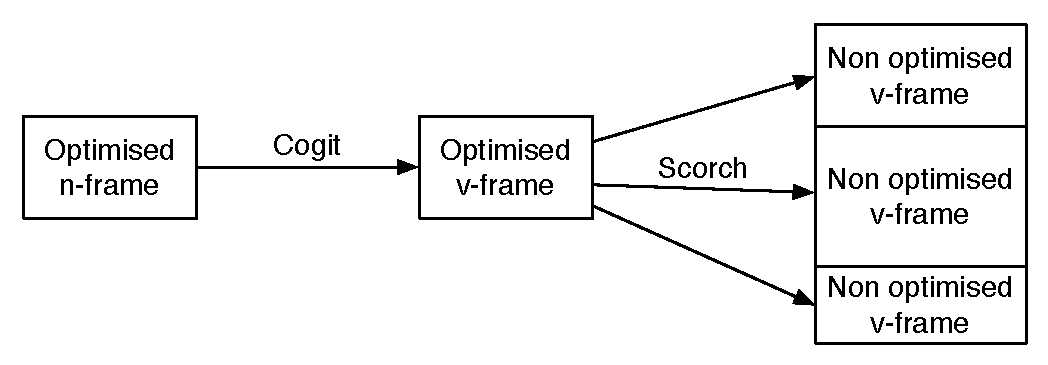
\includegraphics[width=0.8\linewidth]{SFDeoptimisation}
        \caption{Stack frame deoptimisation in two steps}
        \label{fig:SFDeoptimisation}
    \end{center}
\end{figure}

%only stack deopt
When discussing deoptimisation, we deal only with stack recovery (deoptimisation of the optimised frame to the non optimised v-frames). The non optimised v-function is always present and never discarded, so it can be directly set in the non optimised v-frames restored. There is no such thing in our design and implementation as reconstructing non optimised v-function from optimised v-function based on deoptimisation metadata. As far as we know, modern VMs such as V8~\cite{V8} always keep a non-optimised version of each function, so we believe the memory footprint impact of keeping them is acceptable.

\subsection{Deoptimisation management}

%Intro + 2 cases.
Deoptimisation can happen in two main cases. On the one hand, Scorch's optimiser inserts guards(CITE URS OU Dubois) to ensure assumption speculated at optimisation time are valid at runtime, such as the speculation on types. Such guards can fail, requiring deoptimisation of the execution stack to keep executing the application correctly. On the other hand, Smalltalk code can request deoptimisation of the code when manipulating the stack (typically the debugger's code does it).

\paragraph{Guard failure.} When a guard fails, the native code generated by Cogit calls a specific routine in Slang to perform the deoptimisation of the stack. The routine makes sure the frame with the tripping counter is reified so it can be introspected from Smalltalk. Then, the routine performs a virtual call with a selector registered from Smalltalk and the reified stack frame as the receiver. The Smalltalk code lastly calls Scorch deoptimiser's to restore the non optimised stack.

During deoptimisation, the bottom frames are used by the deoptimiser. Just above is a frame for the activation of the virtual call performed by the routine followed by the optimised frame requesting deoptimisation, as shown on figure \ref{fig:DeoptCallBackStack}.

\begin{figure}[h!]
    \begin{center}
        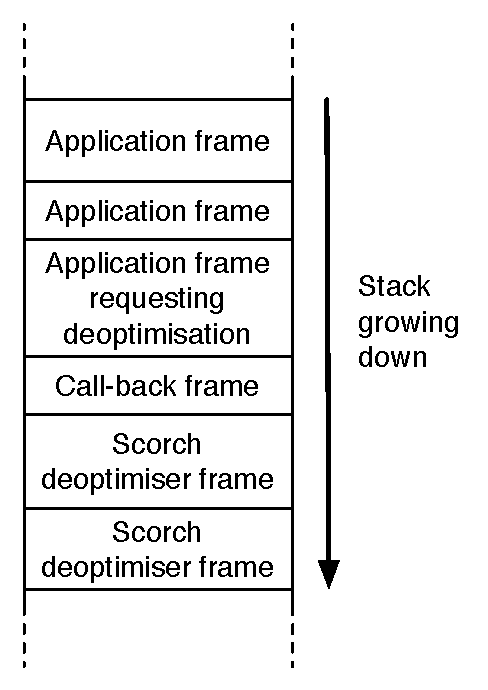
\includegraphics[width=0.4\linewidth]{DeoptCallBackStack}
        \caption{Stack state during guard deoptimisation}
        \label{fig:DeoptCallBackStack}
    \end{center}
\end{figure}

%low-level stack banging issue, in Slang ?
%Flag: FRAMEREIFICATION.

\paragraph{Smalltalk code deoptimisation.}The Smalltalk code can request deoptimisation of specific frames to perform specific operations such as debugging. In this case, the situation is different because:
\begin{enumerate}
	\item The frame to deoptimise is in the middle of the application frames. Instead of having the call-back and deoptimiser frames below the frame to deoptimise on stack, other application frames are present.
	\item The instruction pointer is not on a guard instruction. Although, all instructions where deoptimisation can happen are annotated with deoptimisation metadata, so having the instruction pointer on a non guard instruction does not really change much.
\end{enumerate}

\subsection{Scorch deoptimiser}

%deopt through metadata 
Cogit has reified the optimised n-frame to an optimised v-frame, hence, Scorch's deoptimiser access the optimised v-frame. The frame is necessarily activated on a virtual instruction which is annotated with deoptimisation metadata. The metadata consists of a list of objects to materialize, which allocation have been postponed from runtime to deoptimisation time. As v-frames and closures are reified as objects in Smalltalk, part of those objects to rematerialize are non optimised v-frames and closures. For each field of each object, the metadata specifies if the value is a specific constant, a value to fetch in the optimised v-frame or a reference to one of the other rematerialized object.

\paragraph{Stack edition.}

Once all the non optimised v-frames are reconstructed, the execution stack needs to be edited to use them. This is done using the stack manipulation APIs. Basically, the VM split the current stack page in two, copying one part on another stack page. Deoptimised frames are present in the middle in their single context form, in a similar way to frame divorces described in the previous chapter and as shown in figure \ref{fig:DeoptStacks}.

\begin{figure}[h!]
    \begin{center}
		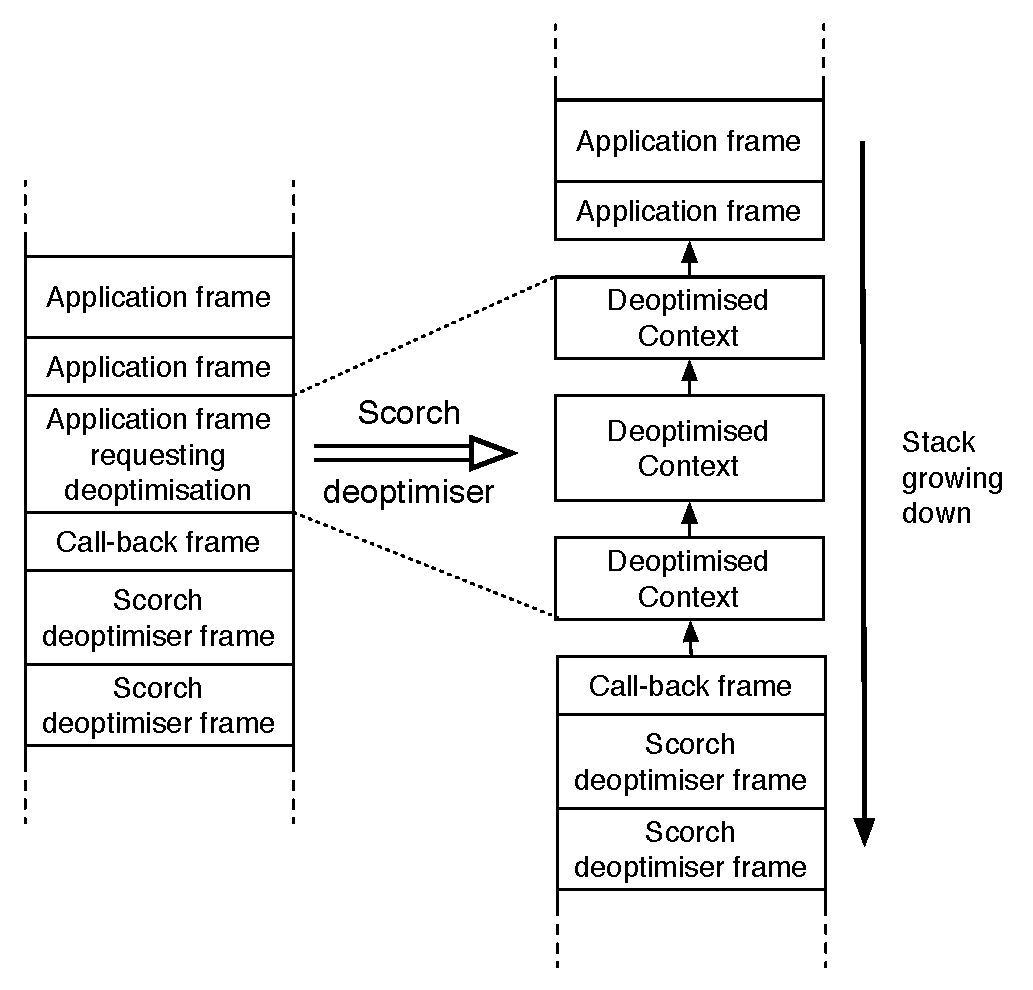
\includegraphics[width=0.80\linewidth]{DeoptStacks}
        \caption{Stack edition}
        \label{fig:DeoptStacks}
    \end{center}
\end{figure}

\paragraph{Discard functions.} When new non optimised functions are installed (for example when a library is loaded), optimisation assumptions may be invalidated because some look-up results cannot be guaranteed any more. In this case, we cannot really iterate over the whole stack and deoptimise all the frames holding invalidated code as it would take a long time (especially multiple stack manipulations may take a while). Instead, Scorch mutates the discarded optimised v-function to hold only guard failures virtual instructions, so optimised v-frames would always trigger deoptimisation upon return. In addition, Scorch requests Cogit to patch all return native instruction pointers of all optimised n-frames representing discarded function activations to a pointer to a specific routine which will trigger deoptimisation upon return.

\paragraph{Execution restart.}

If the deoptimisation happened due to a guard failure (or due to a return to a discarded function), the application needs to resume execution once deoptimisation is performed. In this case, the application frame is just above the call-back frame so returning should resume execution. There is one little detail, a return instruction in Smalltalk pushes the returned value on the caller stack. The deoptimisation call-back returns the top value of the bottom deoptimised frame to resume execution. The bottom deoptimised frame is guaranteed not to be empty as deoptimisation can be only in position in the code where there is necessarily something on stack.

%In those cases, the first deoptimiser frame is just below the bottom restored non optimised v-frame. Returning from the deoptimiser frame to the application is not as easy as for the optimiser call-back. The optimiser is always triggered on a conditional branch and conditionnal branches require a value to test to be on stack. Hence, the optimiser could simply return the value to test and the execution resumes just before the branch. 

%In the case of deoptimisation, the application stack frame could be restored on many different instructions. Especially, it could be restored at an instruction where no value is on stack. Hence to return to the application, the deoptimiser has to perform a special return instruction, which resumes the caller frame execution without pushing any value on its frame.

%%%%%%%%%%%%%%%%%%%%%%%%%%%%%%%%%%%%%%%%%%%%%%%%%%%%%%%%%%%%%%%%%%%%%%%%%%%%%%%%%%%%%%%%%%%%%%%%%%%%%%%%%%%%%%%%%%%%%%%%

\section{Related work}
\label{sec:relatedWorkArch}

This section compares our architecture against existing work. The first section compares the overall Sista architecture versus the meta-tracing and function based architecture. Section \ref{sec:interface} compares our optimised v-function representation against other representation existing in other VMs. Section \ref{sec:codeSharing} discusses how different JIT tiers may or may not share portions of code.

The two research subproblems and their related work are detailed later in the thesis. Chapter \ref{chap:metacircular} discusses how Scorch is able, under specific constraints, to optimise its own code. Chapter \ref{chap:persistance} details how the runtime state, including optimised v-functions, can be persisted across multiple start-ups.

\subsection{Architecture}

Compared to the classical three tier function based architecture described in chapter \ref{chap:stateOfTheArt}, the existing Pharo runtime featured only the first two tiers. The Sista architecture is an implementation of the third tier, the optimising JIT tier. The implementation is however quite different from other VMs. One of the main difference is the split between the high and low level part of the optimising JIT as well as the optimised v-function representation used to communicate between both parts. As far as we know, no other VM splits its optimising JIT this way. The other main difference is Cogit, which in one code base, can be used both as a baseline JIT and as a back-end for the optimising JIT.

The Sista architecture was not designed as a meta-tracing JIT. The main reason is that improving the performance of loop bodies did not seem the right thing to do in the case of Pharo. As explained in the example of section \ref{ss:stackSearch}, if the Smalltalk code executed respects standard Smalltalk coding conventions, most loops just activates a closure. The optimiser needs to optimise code outside of the loop body to be able to inline the closure activation and improve performance. Hence, it is not clear how to implement an efficient meta-tracing JIT for Pharo.

\subsection{Optimised virtual function representation}
\label{sec:interface}

One important difference in the Sista architecture compared to most optimising JITs lies with the optimised v-function representation. Most optimising JIT do not generate optimised v-function but generate only optimised n-functions. As far as we know, no existing baseline JIT is used to compile v-functions optimised using runtime information to optimised n-functions.

\paragraph{Threaded code.}
(CITE ???)
One of the first work in the late 80s to speed up object language virtual machines was in the direction of threaded code interpreters. Such virtual machine would feature a threaded code interpreter instead of a v-function interpreter. A threaded code interpreter is faster to execute code, but require a small compilation time to translate the v-function to its threaded code representation. The threaded code represenation is platform-independent and can be considered as an optimised v-function. The main advantage of the threaded code interpreter is to provide speed-up while keeping the VM platform-independent. Indeed, JIT require a different back-end for each native code supported. 

Work in this direction has mostly vanished for two reasons. Firstly, the execution of v-function through JITs is more efficient than the execution through a threaded interpreter. Secondly, new implementation techniques for v-function interpreters using threaded jumps allowed to massively reduce the performance difference between threaded code interpreter and v-function interpreters.

(CITE ???)
Recently, one problem for VM implementors was to implement JITs for iOS. Apple's policy was forbidding, until very recently, to have a memory page both writable and executable. Such a page is required by a JIT to store the native code it generates so it was not possible to build a JIT running in iOS. One experiment in the Dart VM was to keep the three tier strategy of the function based architecture, but the baseline and optimising JIT would generate an abstract assembly, similar to threaded code. The abstract assembly was then executed quickly by a low-level interpreter, mapping almost one-to-one abstract assembly instructions to native instructions. This solution was not as fast as regular JITs, but it allowed the VM to perform decently under Apple's policy constraints.

\paragraph{Hotspot Graal runtime.}
The VM design the most similar to ours is certainly the Hotspot VM using the Graal compiler~\cite{Oracle13,Dubo13c} as an alternative optimising JIT. In both cases, the baseline JIT and the interpreter are compiled to machine code ahead of time (in our case, from Slang to native code, in Hotspot, from C++ to native code). The optimising JITs, Scorch and Graal, are however written in the language run by the VM and run in the same runtime as the optimised application. 

The main difference still lies with the optimised function representation. Graal generates optimised n-functions in the form of a data structure including the native code and metadata. Graal provides these data structures to the Hotspot VM so it can install them~\cite{Grim13a}. Scorch generates however optimised v-functions, which requires Cogit to compile them. 

With the Graal strategy, it may be possible to produce optimised n-functions slightly faster to execute as the Graal back-end may perform low-level optimisations more aggressively than Cogit. The compilation time may also be slightly better as no optimised v-function representation needs to be created. However, our optimised v-function representation allows us to have a single back-end to maintain for the two JIT tiers in the form of Cogit and as discussed later in the thesis to persist optimised n-functions across multiple start-ups.

\paragraph{WebAssembly.}
Recent Javascript VMs have support for WebAssembly~\cite{WebAssembly}, an abstract assembly code representation for functions. In this case, the VM can take as input two different representations of v-functions. One form is the v-function representation for the language supported, in the case of Javascript the source code of v-functions. The other form, the WebAssembly form, allows the VM to execute v-functions optimised ahead-of-time.

It would be interesting for Scorch to target an optimised v-function representation such as WebAssembly instead of our extended bytecode set. We implemented Scorch to target the extended bytecode set as we could make the architecture work with a limited number of evolutions in Cogit. Being able to compile efficiently a representation such as WebAssembly would require us to add larger extensions to Cogit. One of the goal of our architecture was to limit evolutions on low-level parts of the VM, so the direction we took looked more interesting. Recently, an abstract assembly started to be supported in the Pharo VM, called LowCode~\cite{Salg16a}. It would be interesting, as future work, to investigate if Scorch targeting LowCode would be a valuable option.

\subsection{Sharing code between compiler tiers}
\label{sec:codeSharing}

Most optimising JITs have no code in common with the baseline JIT they extract runtime information from. In our context, Cogit is used both as the baseline JIT and as a back-end for the optimising JIT. Most VM teams keep the back-ends of different JIT tiers independant as each back-end has different constraints. On the one hand, the optimising JIT back-end needs to generate high-performance code in a reasonnable amount of time. On the other hand, the baseline JIT back-end needs to generate code that can be instrospected later as quickly as possible. 

We believe that with Cogit performing a limited number of low-level optimisations while providing n-function instrospection, we can reduce the maintenance cost of the low-level parts of our VM compared to other architecture with a reasonnable performance loss. 

There are two main cases in the litterature where JIT tiers are sharing portions of code.

\paragraph{Webkit VM.}The Javascript Webkit VM~\cite{Webkit15} is one of the only VM where important parts of code are shared between multiple JIT tier. The Webkit VM is different from other VMs as it features four tiers, including two optimising compiler tiers. In the webkit VM, the two optimising JIT tiers are sharing the high-level part of the compiler, but not the back-end. There is some code shared for n-function introspection, but each back-end of each JIT tier is mostly independent from the other tiers.

In our case, we share the back-ends of our two compiler tiers. In addition, the portion of code is shared between a baseline and an optimising JIT and not two optimising JIT tiers.

\paragraph{WebAssembly.}Modern Javascript VMs supports WebAssembly~\cite{WebAssembly}, a abstract assembly representation for functions. In the V8 Javascript engine~\cite{V8}, the back-end of the optimising compiler Turbofan is shared between the WebAssembly compiler and the optimising JIT. This are some similarities with our work as WebAssembly is a representation that could be used to represent optimised v-function. 

In this case, the back-end is shared between two optimising runtime compilers. There is no code shared between the optimising JIT and the baseline JIT. 

%%%%%%%%%%%%%%%%%%%%%%%%%%%%%%%%%%%%%%%%%%%%%%%%%%%%%%%%%%%%%%%%%%%%%%%%%%%%%%%%%%%%%%%%%%%%%%%%%%%%%%%%%%%%%%%%%%%%%%%%

\paragraph{Conclusion.}
The chapter provided an overview of the Sista architecture and detailed the optimisation of functions and deoptimisation of stack frames. The following chapter discusses the evolutions of the Pharo runtime implemented in the context of the thesis.

\ifx\wholebook\relax\else
    \end{document}
\fi
\ifx\wholebook\relax\else

% --------------------------------------------
% Lulu:

    \documentclass[a4paper,12pt,twoside]{../includes/ThesisStyle}

	\usepackage[T1]{fontenc} %%%key to get copy and paste for the code!
%\usepackage[utf8]{inputenc} %%% to support copy and paste with accents for frnehc stuff
\usepackage{times}
\usepackage{ifthen}
\usepackage{xspace}
\usepackage{alltt}
\usepackage{latexsym}
\usepackage{url}            
\usepackage{amssymb}
\usepackage{amsfonts}
\usepackage{amsmath}
\usepackage{stmaryrd}
\usepackage{enumerate}
\usepackage{cite}
%\usepackage[pdftex,colorlinks=true,pdfstartview=FitV,linkcolor=blue,citecolor=blue,urlcolor=blue]{hyperref}
\usepackage{xspace}
%\usepackage{graphicx}
\usepackage{subfigure}
\usepackage[scaled=0.85]{helvet}
        
        
\newcommand{\sepe}{\mbox{>>}}
\newcommand{\pack}[1]{\emph{#1}}
\newcommand{\ozo}{\textsc{oZone}\xspace}
\newcommand\currentissues{\par\smallskip\textbf{Current Issues -- }}

\newboolean{showcomments}
\setboolean{showcomments}{true}
\ifthenelse{\boolean{showcomments}}
  {\newcommand{\bnote}[2]{
	\fbox{\bfseries\sffamily\scriptsize#1}
    {\sf\small$\blacktriangleright$\textit{#2}$\blacktriangleleft$}
    % \marginpar{\fbox{\bfseries\sffamily#1}}
   }
   \newcommand{\cvsversion}{\emph{\scriptsize$-$Id: macros.tex,v 1.1.1.1 2007/02/28 13:43:36 bergel Exp $-$}}
  }
  {\newcommand{\bnote}[2]{}
   \newcommand{\cvsversion}{}
  } 


\newcommand{\here}{\bnote{***}{CONTINUE HERE}}
\newcommand{\nb}[1]{\bnote{NB}{#1}}
\newcommand{\fix}[1]{\bnote{FIX}{#1}}
%%%% add your own macros 

\newcommand{\sd}[1]{\bnote{Stef}{#1}}
\newcommand{\ja}[1]{\bnote{Jannik}{#1}}
\newcommand{\na}[1]{\bnote{Nico}{#1}}
%%% 


\newcommand{\figref}[1]{Figure~\ref{fig:#1}}
\newcommand{\figlabel}[1]{\label{fig:#1}}
\newcommand{\tabref}[1]{Table~\ref{tab:#1}}
\newcommand{\layout}[1]{#1}
\newcommand{\commented}[1]{}
\newcommand{\secref}[1]{Section \ref{sec:#1}}
\newcommand{\seclabel}[1]{\label{sec:#1}}

%\newcommand{\ct}[1]{\textsf{#1}}
\newcommand{\stCode}[1]{\textsf{#1}}
\newcommand{\stMethod}[1]{\textsf{#1}}
\newcommand{\sep}{\texttt{>>}\xspace}
\newcommand{\stAssoc}{\texttt{->}\xspace}

\newcommand{\stBar}{$\mid$}
\newcommand{\stSelector}{$\gg$}
\newcommand{\ret}{\^{}}
\newcommand{\msup}{$>$}
%\newcommand{\ret}{$\uparrow$\xspace}

\newcommand{\myparagraph}[1]{\noindent\textbf{#1.}}
\newcommand{\eg}{\emph{e.g.,}\xspace}
\newcommand{\ie}{\emph{i.e.,}\xspace}
\newcommand{\ct}[1]{{\textsf{#1}}\xspace}


\newenvironment{code}
    {\begin{alltt}\sffamily}
    {\end{alltt}\normalsize}

\newcommand{\defaultScale}{0.55}
\newcommand{\pic}[3]{
   \begin{figure}[h]
   \begin{center}
   \includegraphics[scale=\defaultScale]{#1}
   \caption{#2}
   \label{#3}
   \end{center}
   \end{figure}
}

\newcommand{\twocolumnpic}[3]{
   \begin{figure*}[!ht]
   \begin{center}
   \includegraphics[scale=\defaultScale]{#1}
   \caption{#2}
   \label{#3}
   \end{center}
   \end{figure*}}

\newcommand{\infe}{$<$}
\newcommand{\supe}{$\rightarrow$\xspace}
\newcommand{\di}{$\gg$\xspace}
\newcommand{\adhoc}{\textit{ad-hoc}\xspace}

\usepackage{url}            
\makeatletter
\def\url@leostyle{%
  \@ifundefined{selectfont}{\def\UrlFont{\sf}}{\def\UrlFont{\small\sffamily}}}
\makeatother
% Now actually use the newly defined style.
\urlstyle{leo}



	\usepackage{amsmath,amssymb}             % AMS Math
% \usepackage[french]{babel}
\usepackage[latin1]{inputenc}
\usepackage[T1]{fontenc}
\usepackage[left=1.5in,right=1.3in,top=1.1in,bottom=1.1in,includefoot,includehead,headheight=13.6pt]{geometry}
\renewcommand{\baselinestretch}{1.05}

\usepackage{multicol}

% Table of contents for each chapter

\usepackage[nottoc, notlof, notlot]{tocbibind}
\usepackage{minitoc}
\setcounter{minitocdepth}{1}
\mtcindent=15pt
% Use \minitoc where to put a table of contents

\usepackage{enumitem}

\usepackage{aecompl}

% Glossary / list of abbreviations

%\usepackage[intoc]{nomencl}
%\renewcommand{\nomname}{List of Abbreviations}
%
%\makenomenclature

% My pdf code

\usepackage[pdftex]{graphicx}
\usepackage[a4paper,pagebackref,hyperindex=true]{hyperref}

\usepackage{pgfplotstable,booktabs,colortbl}
\pgfplotsset{compat=1.8}

% Links in pdf
\usepackage{color}
\definecolor{linkcol}{rgb}{0,0,0.4} 
\definecolor{citecol}{rgb}{0.5,0,0} 

% Change this to change the informations included in the pdf file

% See hyperref documentation for information on those parameters

\hypersetup
{
bookmarksopen=true,
pdftitle="Sista: a Metacircular Architecture for Runtime Optimisation Persistence",
pdfauthor="Clement BERA", 
pdfsubject="Thesis", %subject of the document
%pdftoolbar=false, % toolbar hidden
pdfmenubar=true, %menubar shown
pdfhighlight=/O, %effect of clicking on a link
colorlinks=true, %couleurs sur les liens hypertextes
pdfpagemode=None, %aucun mode de page
pdfpagelayout=SinglePage, %ouverture en simple page
pdffitwindow=true, %pages ouvertes entierement dans toute la fenetre
linkcolor=linkcol, %couleur des liens hypertextes internes
citecolor=citecol, %couleur des liens pour les citations
urlcolor=linkcol %couleur des liens pour les url
}

% definitions.
% -------------------

\setcounter{secnumdepth}{3}
\setcounter{tocdepth}{1}

% Some useful commands and shortcut for maths:  partial derivative and stuff

\newcommand{\pd}[2]{\frac{\partial #1}{\partial #2}}
\def\abs{\operatorname{abs}}
\def\argmax{\operatornamewithlimits{arg\,max}}
\def\argmin{\operatornamewithlimits{arg\,min}}
\def\diag{\operatorname{Diag}}
\newcommand{\eqRef}[1]{(\ref{#1})}

\usepackage{rotating}                    % Sideways of figures & tables
%\usepackage{bibunits}
%\usepackage[sectionbib]{chapterbib}          % Cross-reference package (Natural BiB)
%\usepackage{natbib}                  % Put References at the end of each chapter
                                         % Do not put 'sectionbib' option here.
                                         % Sectionbib option in 'natbib' will do.
\usepackage{fancyhdr}                    % Fancy Header and Footer

% \usepackage{txfonts}                     % Public Times New Roman text & math font
  
%%% Fancy Header %%%%%%%%%%%%%%%%%%%%%%%%%%%%%%%%%%%%%%%%%%%%%%%%%%%%%%%%%%%%%%%%%%
% Fancy Header Style Options

\pagestyle{fancy}                       % Sets fancy header and footer
\fancyfoot{}                            % Delete current footer settings

%\renewcommand{\chaptermark}[1]{         % Lower Case Chapter marker style
%  \markboth{\chaptername\ \thechapter.\ #1}}{}} %

%\renewcommand{\sectionmark}[1]{         % Lower case Section marker style
%  \markright{\thesection.\ #1}}         %

\fancyhead[LE,RO]{\bfseries\thepage}    % Page number (boldface) in left on even
% pages and right on odd pages
\fancyhead[RE]{\bfseries\nouppercase{\leftmark}}      % Chapter in the right on even pages
\fancyhead[LO]{\bfseries\nouppercase{\rightmark}}     % Section in the left on odd pages

\let\headruleORIG\headrule
\renewcommand{\headrule}{\color{black} \headruleORIG}
\renewcommand{\headrulewidth}{1.0pt}
\usepackage{colortbl}
\arrayrulecolor{black}

\fancypagestyle{plain}{
  \fancyhead{}
  \fancyfoot{}
  \renewcommand{\headrulewidth}{0pt}
}

\usepackage{algorithm}
\usepackage[noend]{algorithmic}

%%% Clear Header %%%%%%%%%%%%%%%%%%%%%%%%%%%%%%%%%%%%%%%%%%%%%%%%%%%%%%%%%%%%%%%%%%
% Clear Header Style on the Last Empty Odd pages
\makeatletter

\def\cleardoublepage{\clearpage\if@twoside \ifodd\c@page\else%
  \hbox{}%
  \thispagestyle{empty}%              % Empty header styles
  \newpage%
  \if@twocolumn\hbox{}\newpage\fi\fi\fi}

\makeatother
 
%%%%%%%%%%%%%%%%%%%%%%%%%%%%%%%%%%%%%%%%%%%%%%%%%%%%%%%%%%%%%%%%%%%%%%%%%%%%%%% 
% Prints your review date and 'Draft Version' (From Josullvn, CS, CMU)
\newcommand{\reviewtimetoday}[2]{\special{!userdict begin
    /bop-hook{gsave 20 710 translate 45 rotate 0.8 setgray
      /Times-Roman findfont 12 scalefont setfont 0 0   moveto (#1) show
      0 -12 moveto (#2) show grestore}def end}}
% You can turn on or off this option.
% \reviewtimetoday{\today}{Draft Version}
%%%%%%%%%%%%%%%%%%%%%%%%%%%%%%%%%%%%%%%%%%%%%%%%%%%%%%%%%%%%%%%%%%%%%%%%%%%%%%% 

\newenvironment{maxime}[1]
{
\vspace*{0cm}
\hfill
\begin{minipage}{0.5\textwidth}%
%\rule[0.5ex]{\textwidth}{0.1mm}\\%
\hrulefill $\:$ {\bf #1}\\
%\vspace*{-0.25cm}
\it 
}%
{%

\hrulefill
\vspace*{0.5cm}%
\end{minipage}
}

\let\minitocORIG\minitoc
\renewcommand{\minitoc}{\minitocORIG \vspace{1.5em}}

\usepackage{multirow}
\usepackage{slashbox}

\newenvironment{bulletList}%
{ \begin{list}%
	{$\bullet$}%
	{\setlength{\labelwidth}{25pt}%
	 \setlength{\leftmargin}{30pt}%
	 \setlength{\itemsep}{\parsep}}}%
{ \end{list} }

\newtheorem{definition}{D�finition}
\renewcommand{\epsilon}{\varepsilon}

% centered page environment

\newenvironment{vcenterpage}
{\newpage\vspace*{\fill}\thispagestyle{empty}\renewcommand{\headrulewidth}{0pt}}
{\vspace*{\fill}}



	\graphicspath{{.}{../figures/}}
	\begin{document}
\fi

\chapter{Runtime evolutions}
\label{chap:runtimeEvolution}
\minitoc

%Generic intro
To support the architecture described in the previous chapter, the Pharo runtime had to evolve. We distinguish two kind of evolutions. Some evolutions were required to support the architecture, the Sista runtime could not work without those features. Other evolutions were not mandatory, the Sista architecture could have worked without these features, but each of them are really important for the Scorch optimiser to be able to generate optimised code.

%%%%%%%%%%%%%%%%%%%%%%%%%%%%%%%%%%%%%%%%%%%%%%%%%%%%%%%%%%%%%%%%%%%%%%%%%%%%%%%%%%%%%%%%%%%%%%%%%%%%%%%%%%%%%%%%%%%%%%%%%%%%%%%%%%%%
%%%%%%%%%%%%%%%%%%%%%%%%%%%%%%%%%%%%%%%%%%%%%%%%%%%%%%%%%%%%%%%%%%%%%%%%%%%%%%%%%%%%%%%%%%%%%%%%%%%%%%%%%%%%%%%%%%%%%%%%%%%%%%%%%%%%

\section{Required language evolutions}

Five major evoluations were required to have the Sista architecture up and running:
\begin{enumerate}
	\item Cogit were extended to detect hot spot through profiling counters.
	\item The interpreter and Cogit were extended to be able to execute and compile the additional instructions of the extended bytecode set.
	\item Two VM call-backs to announce to Scorch hot spot detection and guard failures were added.
	\item A new primitive was introduce for Cogit to instrospect the n-functions and provide type and basic block usage.
	\item The Scorch framework, including the optimiser and the deoptimiser, were introduced.
\end{enumerate}

\subsection{Profiling counters}

As described in the previous chapter, Cogit was extended to support conditionnal compilation. Based on a bit in a v-function's header, Cogit generates a n-function with or without profiling counters. Profiling counters induce overhead, which can be significant enough to be seen in some benchmarks (this will be discussed in (benchs are in section persistance, or maybe external)). 

Based on \cite{Arn02}, the profiling counter strategy consisted in the addition of counters to conditional branches, to provide basic block usage information instead of just detecting hot spots. Every finite loop requires a branch to stop the loop iteration and most recursive code requires a branch to stop the recursion, so the main cases for which we wanted to detect hot spots for are covered. Each time the execution flow reaches a conditional branch in a n-function, it increases the profiling counter by one, compares the counter value to a threshold and jumps to the tripping counter routine if the threshold is reached. If the threshold is not reached, the conditional branch is performed, but the branch is not taken, a second counter is incremented by one to provide later basic block usage information.

The main issue we had to deal with when implementing profiling counters is the location of the counters and the access to the counters. Indeed, our first naive implementation was to put the counter values directly inlined in the native code. That was a terrible idea as every write near executable code flushes part of the processor instruction cache, leading to horrible performance. In the end, we changed the logic to allocate a pinned array\footnote{A pinned object is an object that can never be moved in memory. For example, the garbage collector cannot move it.} for each n-function requiring counters. The pinned array is therefore on heap, far from executable code, and contains all the counter values. As the array is pinned, the native code can access the array and each of its fields (each counter) through a constant address. This is very nice as the native code can be efficient by using constant addresses and the n-function does not require any metadata~\footnote{References to non pinned objects from n-function normally require metadata to update the reference when the object is moved in memory, typically by the garbage collector.}.

\subsection{Extended bytecode set}

The Sista architecture required an extended bytecode set to support all the new operations permitted only in optimised v-functions. The new operations were described in one of our IWST paper\cite{Bera14a}. The extended bytecode set design relies on the assumption that only a small number of new instructions are needed for Cogit to produce efficient machine code. Four main kind of instructions were added into the bytecode set:
\begin{itemize}
\item \textbf{Guards}: guards are used to ensure a specific object has a given type, else they trigger dynamic deoptimization.
\item \textbf{Object unchecked accesses}: normally variable-sized objects such as arrays or byte arrays require type and bounds checks to allow a program to access their fields. Unchecked access directly reads the field of an object without any checks. Instructions to access the size of a variable-sized object without type-check or format-check (The object format defines if the object holds raw data such as bytes or pointers) are included.
\item \textbf{Unchecked arithmetics}: Arithmetic operations needs to check for the operand types to know what arithmetic operation to call (on integers, double, etc.). Unchecked operations are typed and do not need these check. In addition, unchecked operations do not do an overflow check and are converted efficiently to machine code conditional branches if followed by a conditional jump.
\item \textbf{Unchecked object allocation and stores}: Normal object allocations do many different things in addition to memory allocation, such as the initialization of all fields to \ct{nil} which is not needed if all fields are set immediately after to other values. Normal stores into objects go through a write barrier to make sure that the store does not break any garbage collector invariant. Such a write barrier can be ignored in specific cases, for example when doing a store in an object that has just been allocated, because it is guaranteed to be in the young object space.
\end{itemize}

As the optimized methods are represented as bytecodes, they can potentially be executed by the VM interpreter. However, as discussed in the previous chapter, we made sure that it was very uncommon. Improving the performance to speed-up the bytecode interpreter or to speed-up the machine code generated using Cogit are two different tasks that may conflict with one another. We designed the extended bytecode set so the machine code generated by Cogit is as efficient as possible, not really considering the speed of the interpretation of such v-functions.

\subsection{Call-backs}

%KEEP WRITING FROM HERE

%As in our implementation the runtime optimizer and deoptimizer are implemented in Smalltalk and not in the virtual machine itself, we needed to introduce callbacks activated by the virtual machine to activate the optimizer and the deoptimizer. 

%These callbacks use the reification of stack frames available for the debugger to inform the language which frame had its method detected as a hot spot and which frame has to be deoptimized.

%END WRITING HERE

\subsection{Machine code introspection}

%what does the primitive + intro
To extract runtime information from a n-function, we added a new primitive method called \emph{sendAndBranchData}. SendAndBranchData is activated with no arguments and fails if the receiver is not a v-function. If the v-function was compiled by Cogit and therefore has an associated n-function, the primitive answers the types met at each inline cache and the values of the counters at each branch. This information can be then used by Scorch to speculate on variable type and basic block usage. 

%reading the cache/counter through 
The cache and counter values are read by reusing Cogit's API for relinking. Indeed, each virtual call in non optimised n-functions are implemented with inline caches~\cite{Deut84a,Holz91a}, relinked at runtime each type a new receiver type is met for the call. Each profiling counter native code is followed by a call to the hot spot detection Slang routine, this call is annotated as a relative call is used to call the routine and Cogit needs to relink it when it moves n-functions in memory (typically when compacting the zone where n-functions are). Each native instruction annotation contains a mapping from the native instruction pointer to the virtual instruction pointer, which is used for other purpose such as stack reification or debugging.

%Result of primitive
The new primitive iterates over the n-function, collecting for each virtual call and each conditionnal branch the virtual instruction pointer as well as respectively type and profiling information. Because the data is collected from Slang, it's not convenient to build complex data structure using multiple different kind of objects (Each object's class internal representation would need to be specifically known by both the VM and the language). To keep things simple, the primitive answers an array of array, each inner array containing the virtual program counter of the instruction, and a list of types and v-functions targetted by the inline cache or the number of times each branch has been taken.

\subsection{Runtime optimiser and deoptimiser}

TODO

%Explain simple behavior.

%Maybe it makes sense to say Context are the same as objects.

%Doc: my blog post + sista arch

END TODO

%%%%%%%%%%%%%%%%%%%%%%%%%%%%%%%%%%%%%%%%%%%%%%%%%%%%%%%%%%%%%%%%%%%%%%%%%%%%%%%%%%%%%%%%%%%%%%%%%%%%%%%%%%%%%%%%%%%%%%%%%%%%%%%%%%%%
%%%%%%%%%%%%%%%%%%%%%%%%%%%%%%%%%%%%%%%%%%%%%%%%%%%%%%%%%%%%%%%%%%%%%%%%%%%%%%%%%%%%%%%%%%%%%%%%%%%%%%%%%%%%%%%%%%%%%%%%%%%%%%%%%%%%

\section{Optional language evolutions}


Five major evolutions were introduced in the language in addition to the required evolutions to allow Scorch to produce more efficient optimised v-functions:
\begin{enumerate}
	\item A new memory manager for efficient n-function generation.
	\item A new bytecode set to leverage encoding limitations.
	\item A register allocation algorithm in Cogit.
	\item A write barrier feature to be able to mark object as read-only.
	\item A new closure implementation to be able to optimiser closure more efficiently.
\end{enumerate}

\subsection{New memory manager}

%pb with existing representation
The first version of the Sista architecture was built on the existing VM with a minimum number of modifications. One of the main issue met was related to memory manager, especially the memory representation of objects. The existing memory manager was designed and implemented before the implementation of Cogit, for an interpreter-based VM. The representation of object did not allow Cogit to produce efficient n-function.

%existing class access
One problem for example was the encoding of the class field in an object. It could be encoded in three different ways:
\begin{itemize}
	\item \emph{Immediate classes:} A very limited subset of classes, included \ct{SmallInteger}, have their instances encoded in the pointer to the object itself. As all objects are aligned in memory for efficient access to their fields, the last few bits (the exact number depends on the alignment) of a pointer to an object are never set. By using different numbers on those last few bits, the memory manager can encode a class identifier. \ct{SmallInteger} for example are encoded by setting the last bit of the pointer.
	\item \emph{Compact classes:} A limited set of classes, up to 15 classes, had their instances encoding the class as an index in a 4-bits field in the first word of the object's header. The memory manager had access to an array mapping the indexes to the actual classes.
	\item \emph{Other classes:} All the other instances encode their class as a pointer to the class object, encoded in an extra pointer-sized field in the header of the object.
\end{itemize}

%existing class access pb in n-functions
Cogit frequently to compiles type-checks, mostly in the context of inline caching in non optimised n-functions and in the context of deoptimisation guards in optimised n-functions. For each type-check, the native code generated needs three paths to find out which one of the three encodings is used for the instance which is type-checked, to finally compare it against the expected type. In addition, as most instances encode their class as a pointer to a class object while class objects can be moved by the garbage collector in memory, cogit needs to annotate the expected type to correctly update the pointer value during garbage collection. Overall both the generated n-function and the garbage collector get slowed by the memory representation.

%Spur and problem solving
To solve this problem, a new memory manager was implemented and deployed in production~\cite{Mir15a}. The new representation of objects in memory allows the generation of very efficient n-functions. For example, there is now only two ways for an instance to access its class, the class is either immediate or compact. Compact classes indexes are stored in the instances in a 22-bit fields, allowing over four millions different classes. As all references to classes are now through an indirection index, type-checks do not require Cogit to annotate them and the garbage collector can ignore them.

%other pbs soled
In addition to allowing the generation of efficient n-functions, other problems non directly related to the thesis were present in the existing memory manager (poor support for large heaps, slow scavenges, etc.) which were solved with the new memory manager.

% pinned objects ??? I don't know if it's worth going into details there.

\subsection{New bytecode set}

TODO 

%\cite{Bera14a}
%New bytecode set needs to be discussed (not only extensions).



\subsection{Register allocation}

%Linear scan and reg alloc, plus branches

END TODO

\subsection{Read-only objects}

One of the main problem encountered while trying to improve the performance of the optimised v-functions generated by Scorch was literal mutability. In most programming languages, if the program executes a simple double addition between two double constants the compiler can compute at compile-time the result. In Pharo, as literals are mutable, one of the double constant may be accessed through reflective APIs and mutated into another boxed double, invalidating the compile-time result. 

To solve the problem, we introduced a feature, called read-only objects~\cite{Bera16b}. With this feature, a program can mark any object as read-only. Such read-only objects cannot be modified unless the program explicitly revert them to a writable state. Any attempt to modify a read-only object calls a specific v-function which can be modified from Smalltalk to have the behavior desired by the programmer. The modification failure routine can, for example, revert the object to a writable state, perform the modification and notify a list of subscribers that the modification happened. This feature was introduced with limited overhead to the existing runtime~\cite{Bera16b}. 

Literals can now all be read-only objects by default. Any attempt to modify a read-only literal is caught by the runtime and can notify Scorch just after performing the modification. If the literal was used for compile-time computation, corresponding optimised v-functions are discarded. Thanks to this technique, traditional compiler optimisations can be applied to Smalltalk.

\subsection{Closure implementation}

TODO

%The second major issue encountered was related to the closure implementation. 

%FullBlock
%Doc: ? well... the FullBlock talk

END TODO


\ifx\wholebook\relax\else
    \end{document}
\fi
\ifx\wholebook\relax\else

% --------------------------------------------
% Lulu:

    \documentclass[a4paper,12pt,twoside]{../includes/ThesisStyle}

	\usepackage[T1]{fontenc} %%%key to get copy and paste for the code!
%\usepackage[utf8]{inputenc} %%% to support copy and paste with accents for frnehc stuff
\usepackage{times}
\usepackage{ifthen}
\usepackage{xspace}
\usepackage{alltt}
\usepackage{latexsym}
\usepackage{url}            
\usepackage{amssymb}
\usepackage{amsfonts}
\usepackage{amsmath}
\usepackage{stmaryrd}
\usepackage{enumerate}
\usepackage{cite}
%\usepackage[pdftex,colorlinks=true,pdfstartview=FitV,linkcolor=blue,citecolor=blue,urlcolor=blue]{hyperref}
\usepackage{xspace}
%\usepackage{graphicx}
\usepackage{subfigure}
\usepackage[scaled=0.85]{helvet}
        
        
\newcommand{\sepe}{\mbox{>>}}
\newcommand{\pack}[1]{\emph{#1}}
\newcommand{\ozo}{\textsc{oZone}\xspace}
\newcommand\currentissues{\par\smallskip\textbf{Current Issues -- }}

\newboolean{showcomments}
\setboolean{showcomments}{true}
\ifthenelse{\boolean{showcomments}}
  {\newcommand{\bnote}[2]{
	\fbox{\bfseries\sffamily\scriptsize#1}
    {\sf\small$\blacktriangleright$\textit{#2}$\blacktriangleleft$}
    % \marginpar{\fbox{\bfseries\sffamily#1}}
   }
   \newcommand{\cvsversion}{\emph{\scriptsize$-$Id: macros.tex,v 1.1.1.1 2007/02/28 13:43:36 bergel Exp $-$}}
  }
  {\newcommand{\bnote}[2]{}
   \newcommand{\cvsversion}{}
  } 


\newcommand{\here}{\bnote{***}{CONTINUE HERE}}
\newcommand{\nb}[1]{\bnote{NB}{#1}}
\newcommand{\fix}[1]{\bnote{FIX}{#1}}
%%%% add your own macros 

\newcommand{\sd}[1]{\bnote{Stef}{#1}}
\newcommand{\ja}[1]{\bnote{Jannik}{#1}}
\newcommand{\na}[1]{\bnote{Nico}{#1}}
%%% 


\newcommand{\figref}[1]{Figure~\ref{fig:#1}}
\newcommand{\figlabel}[1]{\label{fig:#1}}
\newcommand{\tabref}[1]{Table~\ref{tab:#1}}
\newcommand{\layout}[1]{#1}
\newcommand{\commented}[1]{}
\newcommand{\secref}[1]{Section \ref{sec:#1}}
\newcommand{\seclabel}[1]{\label{sec:#1}}

%\newcommand{\ct}[1]{\textsf{#1}}
\newcommand{\stCode}[1]{\textsf{#1}}
\newcommand{\stMethod}[1]{\textsf{#1}}
\newcommand{\sep}{\texttt{>>}\xspace}
\newcommand{\stAssoc}{\texttt{->}\xspace}

\newcommand{\stBar}{$\mid$}
\newcommand{\stSelector}{$\gg$}
\newcommand{\ret}{\^{}}
\newcommand{\msup}{$>$}
%\newcommand{\ret}{$\uparrow$\xspace}

\newcommand{\myparagraph}[1]{\noindent\textbf{#1.}}
\newcommand{\eg}{\emph{e.g.,}\xspace}
\newcommand{\ie}{\emph{i.e.,}\xspace}
\newcommand{\ct}[1]{{\textsf{#1}}\xspace}


\newenvironment{code}
    {\begin{alltt}\sffamily}
    {\end{alltt}\normalsize}

\newcommand{\defaultScale}{0.55}
\newcommand{\pic}[3]{
   \begin{figure}[h]
   \begin{center}
   \includegraphics[scale=\defaultScale]{#1}
   \caption{#2}
   \label{#3}
   \end{center}
   \end{figure}
}

\newcommand{\twocolumnpic}[3]{
   \begin{figure*}[!ht]
   \begin{center}
   \includegraphics[scale=\defaultScale]{#1}
   \caption{#2}
   \label{#3}
   \end{center}
   \end{figure*}}

\newcommand{\infe}{$<$}
\newcommand{\supe}{$\rightarrow$\xspace}
\newcommand{\di}{$\gg$\xspace}
\newcommand{\adhoc}{\textit{ad-hoc}\xspace}

\usepackage{url}            
\makeatletter
\def\url@leostyle{%
  \@ifundefined{selectfont}{\def\UrlFont{\sf}}{\def\UrlFont{\small\sffamily}}}
\makeatother
% Now actually use the newly defined style.
\urlstyle{leo}



	\usepackage{amsmath,amssymb}             % AMS Math
% \usepackage[french]{babel}
\usepackage[latin1]{inputenc}
\usepackage[T1]{fontenc}
\usepackage[left=1.5in,right=1.3in,top=1.1in,bottom=1.1in,includefoot,includehead,headheight=13.6pt]{geometry}
\renewcommand{\baselinestretch}{1.05}

\usepackage{multicol}

% Table of contents for each chapter

\usepackage[nottoc, notlof, notlot]{tocbibind}
\usepackage{minitoc}
\setcounter{minitocdepth}{1}
\mtcindent=15pt
% Use \minitoc where to put a table of contents

\usepackage{enumitem}

\usepackage{aecompl}

% Glossary / list of abbreviations

%\usepackage[intoc]{nomencl}
%\renewcommand{\nomname}{List of Abbreviations}
%
%\makenomenclature

% My pdf code

\usepackage[pdftex]{graphicx}
\usepackage[a4paper,pagebackref,hyperindex=true]{hyperref}

\usepackage{pgfplotstable,booktabs,colortbl}
\pgfplotsset{compat=1.8}

% Links in pdf
\usepackage{color}
\definecolor{linkcol}{rgb}{0,0,0.4} 
\definecolor{citecol}{rgb}{0.5,0,0} 

% Change this to change the informations included in the pdf file

% See hyperref documentation for information on those parameters

\hypersetup
{
bookmarksopen=true,
pdftitle="Sista: a Metacircular Architecture for Runtime Optimisation Persistence",
pdfauthor="Clement BERA", 
pdfsubject="Thesis", %subject of the document
%pdftoolbar=false, % toolbar hidden
pdfmenubar=true, %menubar shown
pdfhighlight=/O, %effect of clicking on a link
colorlinks=true, %couleurs sur les liens hypertextes
pdfpagemode=None, %aucun mode de page
pdfpagelayout=SinglePage, %ouverture en simple page
pdffitwindow=true, %pages ouvertes entierement dans toute la fenetre
linkcolor=linkcol, %couleur des liens hypertextes internes
citecolor=citecol, %couleur des liens pour les citations
urlcolor=linkcol %couleur des liens pour les url
}

% definitions.
% -------------------

\setcounter{secnumdepth}{3}
\setcounter{tocdepth}{1}

% Some useful commands and shortcut for maths:  partial derivative and stuff

\newcommand{\pd}[2]{\frac{\partial #1}{\partial #2}}
\def\abs{\operatorname{abs}}
\def\argmax{\operatornamewithlimits{arg\,max}}
\def\argmin{\operatornamewithlimits{arg\,min}}
\def\diag{\operatorname{Diag}}
\newcommand{\eqRef}[1]{(\ref{#1})}

\usepackage{rotating}                    % Sideways of figures & tables
%\usepackage{bibunits}
%\usepackage[sectionbib]{chapterbib}          % Cross-reference package (Natural BiB)
%\usepackage{natbib}                  % Put References at the end of each chapter
                                         % Do not put 'sectionbib' option here.
                                         % Sectionbib option in 'natbib' will do.
\usepackage{fancyhdr}                    % Fancy Header and Footer

% \usepackage{txfonts}                     % Public Times New Roman text & math font
  
%%% Fancy Header %%%%%%%%%%%%%%%%%%%%%%%%%%%%%%%%%%%%%%%%%%%%%%%%%%%%%%%%%%%%%%%%%%
% Fancy Header Style Options

\pagestyle{fancy}                       % Sets fancy header and footer
\fancyfoot{}                            % Delete current footer settings

%\renewcommand{\chaptermark}[1]{         % Lower Case Chapter marker style
%  \markboth{\chaptername\ \thechapter.\ #1}}{}} %

%\renewcommand{\sectionmark}[1]{         % Lower case Section marker style
%  \markright{\thesection.\ #1}}         %

\fancyhead[LE,RO]{\bfseries\thepage}    % Page number (boldface) in left on even
% pages and right on odd pages
\fancyhead[RE]{\bfseries\nouppercase{\leftmark}}      % Chapter in the right on even pages
\fancyhead[LO]{\bfseries\nouppercase{\rightmark}}     % Section in the left on odd pages

\let\headruleORIG\headrule
\renewcommand{\headrule}{\color{black} \headruleORIG}
\renewcommand{\headrulewidth}{1.0pt}
\usepackage{colortbl}
\arrayrulecolor{black}

\fancypagestyle{plain}{
  \fancyhead{}
  \fancyfoot{}
  \renewcommand{\headrulewidth}{0pt}
}

\usepackage{algorithm}
\usepackage[noend]{algorithmic}

%%% Clear Header %%%%%%%%%%%%%%%%%%%%%%%%%%%%%%%%%%%%%%%%%%%%%%%%%%%%%%%%%%%%%%%%%%
% Clear Header Style on the Last Empty Odd pages
\makeatletter

\def\cleardoublepage{\clearpage\if@twoside \ifodd\c@page\else%
  \hbox{}%
  \thispagestyle{empty}%              % Empty header styles
  \newpage%
  \if@twocolumn\hbox{}\newpage\fi\fi\fi}

\makeatother
 
%%%%%%%%%%%%%%%%%%%%%%%%%%%%%%%%%%%%%%%%%%%%%%%%%%%%%%%%%%%%%%%%%%%%%%%%%%%%%%% 
% Prints your review date and 'Draft Version' (From Josullvn, CS, CMU)
\newcommand{\reviewtimetoday}[2]{\special{!userdict begin
    /bop-hook{gsave 20 710 translate 45 rotate 0.8 setgray
      /Times-Roman findfont 12 scalefont setfont 0 0   moveto (#1) show
      0 -12 moveto (#2) show grestore}def end}}
% You can turn on or off this option.
% \reviewtimetoday{\today}{Draft Version}
%%%%%%%%%%%%%%%%%%%%%%%%%%%%%%%%%%%%%%%%%%%%%%%%%%%%%%%%%%%%%%%%%%%%%%%%%%%%%%% 

\newenvironment{maxime}[1]
{
\vspace*{0cm}
\hfill
\begin{minipage}{0.5\textwidth}%
%\rule[0.5ex]{\textwidth}{0.1mm}\\%
\hrulefill $\:$ {\bf #1}\\
%\vspace*{-0.25cm}
\it 
}%
{%

\hrulefill
\vspace*{0.5cm}%
\end{minipage}
}

\let\minitocORIG\minitoc
\renewcommand{\minitoc}{\minitocORIG \vspace{1.5em}}

\usepackage{multirow}
\usepackage{slashbox}

\newenvironment{bulletList}%
{ \begin{list}%
	{$\bullet$}%
	{\setlength{\labelwidth}{25pt}%
	 \setlength{\leftmargin}{30pt}%
	 \setlength{\itemsep}{\parsep}}}%
{ \end{list} }

\newtheorem{definition}{D�finition}
\renewcommand{\epsilon}{\varepsilon}

% centered page environment

\newenvironment{vcenterpage}
{\newpage\vspace*{\fill}\thispagestyle{empty}\renewcommand{\headrulewidth}{0pt}}
{\vspace*{\fill}}



	\graphicspath{{.}{../figures/}}
	\begin{document}
\fi

\chapter{Metacircular optimising JIT}
\label{chap:metacircular}
\minitoc

%Intro
By design, Scorch's optimiser and deoptimiser are written in Smalltalk and are running in the same runtime than the optimised application. This design leads to multiple problems similar to the ones existing in metacircular virtual machines. 

%single-threaded -> for comparison with Graal and co later
As Pharo is currently single-threaded, it is not possible to run Scorch in a concurrent native thread. To optimise code, Scorch requires either to temporarily interrupt the application green thread or to postpone the optimisation to a background-priority green thread as described in section \ref{sec:optModes}. The deoptimiser cannot however postpone the deoptimisation of a frame as it would block completely the running application. The deoptimiser has necessarily to interrupt the application green thread until deoptimisation is finished.

%introduction of the main issue
Hot spots can be detected in any Smalltalk code using conditionnal branches, including Scorch optimiser code itself (as Scorch is written in Smalltalk). When a hot spot is detected in the optimiser code, the optimiser interrupts itself and starts to optimise one of its own function. While doing so, the same hot spot may be detected again before any optimised function is installed, leading the optimiser to interrupt itself repeatedly. 

As Scorch deoptimiser is written in Smalltalk, its code base may get optimised. One of the optimisation-time speculation may be incorrect at runtime, leading the deoptimiser to require the deoptimisation of one of its own frame. In this case, the deoptimiser calls itself on one of its own frame, which may require to deoptimise a frame for the same function, leading the deoptimiser to call itself repeatedly. 

We call the \emph{infinite recursion} problem this issue where the optimiser or the deoptimiser respectively calls itself. The issue is detailed for each case in the first two sections.

%Different constraint so different solutions
The optimiser and deoptimiser have different constraints. It is possible to disable temporarily the optimiser while the application is running. In the worst case, a disabled optimiser leads to some functions not to be optimised, but the application keeps running correctly. However, the deoptimiser cannot be disabled temporarily while the application is running as the deoptimiser may be needed to keep executing code. As the optimiser and the deoptimiser have different constraints, they need different solutions for the infinite recursion problem.

%Outline and solution
This chapter explains the design used to avoid the infinite recursion issue in both the optimiser and the deoptimiser. The problem is solved in the optimiser by temporarily disabling it in specific circumstances. The deoptimiser solves the problem by using a code base completely independent from the rest of the system that cannot be optimised, hence it never requires to be deoptimised. The last section discuss similar design issues in other VMs and compares our solution to other solutions when relevant.

%%%%%%%%%%%%%%%%%%%%%%%%%%%%%%%%%%%%%%%%%%%%%%%%%%%%%%%%%%%%%%%%%%%%%%%%%%%%%%%%%%%%%%%%%%%%%%%%%%%%%%%%%%%%%%%%%%%%%%%%%%%%%

\section{Scorch optimiser}

%Intro, what Scorch optimiser does and critical mode.
Scorch optimiser is activated by the VM when a hot spot is detected. As Pharo is single-threaded, the optimiser is activated by interrupting the application green thread. The optimiser chooses, based on the current stack, a v-function to optimise.  Once the v-function to optimise is chosen, the optimiser gets started in critical mode: it attempts to generate an optimised v-function in a limited time period. If it succeeds, the optimised v-function is installed and used by further calls on the function. If the optimiser fails to generate the optimised v-function in the limited time period, it adds the v-function to a background compilation queue. In any case, the application is then resumed. When the application becomes idle, if the background compilation queue is not empty, Scorch gets activated in background mode. It produces and installs optimised v-functions for each function in the compilation queue without any time limit. 

\subsection{Infinite recursion issue}

%repeat problem for optimiser
As Scorch optimiser is written in Smalltalk, it can theoretically optimise its own code. In practice, if it happens, it may lead to an infinite recursion. Indeed, each time Scorch tries to optimise a function, before reaching the point where it can install the optimised function, it may interrupt itself to start optimising one of its own function. If a hot spot is detected in the optimiser code each time it attempts to optimise anything, then the optimiser never reaches the point where it can install an optimised function.

Figure \ref{fig:InfiniteRecursionOptPb} shows the problem. On the left, in the normal optimisation flow, the application is interrupted when a hot spot is detected, the optimiser generates an optimised v-function, installs it and the application resumes. On the right, in the infinite recursion issue, the application is also interrupted when a hot spot is detected, but while the optimiser is generating an optimised function, a hot spot is detected in the optimiser code. The optimiser then restarts to optimise one of its own function, but another hot spot is detected in the optimiser code. The optimiser keeps restarting the optimisation of one of its function.

\begin{figure}[h!]
    \begin{center}
        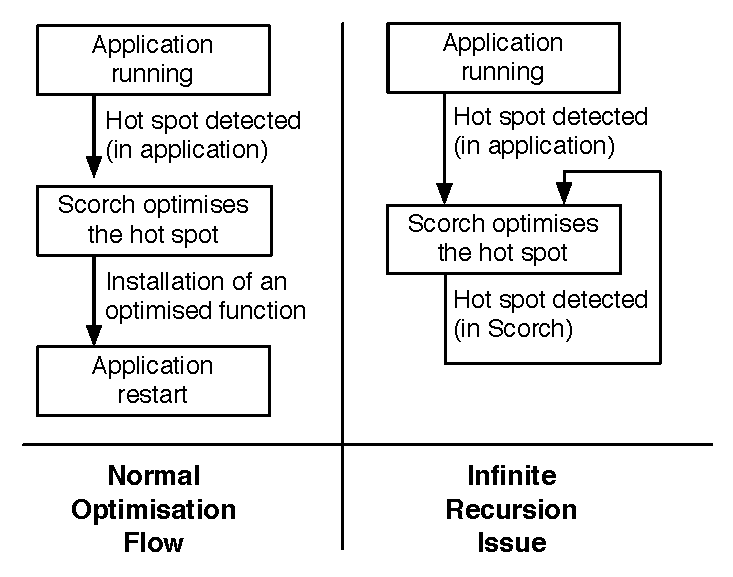
\includegraphics[width=0.65\linewidth]{InfiniteRecursionOptPb}
        \caption{Infinite recursion problem during optimisation}
        \label{fig:InfiniteRecursionOptPb}
    \end{center}
\end{figure}

In practice, the infinite recursion issue leads to a massive performance loss.

%slow down - critical
In critical mode, the optimiser has a limited time period to optimise code. If the infinite recursion issue happens, the optimiser spins until the time period ends as shown in figure \ref{fig:InfiniteRecursionOptPbCritical}. The application is then resumed without any optimised function installed. The application gets drastically slower as it gets interrupted for the full critical mode time period without gaining any performance from those interruptions.


\begin{figure}
    \begin{center}
		\subfigure[Critical mode]{\label{fig:InfiniteRecursionOptPbCritical}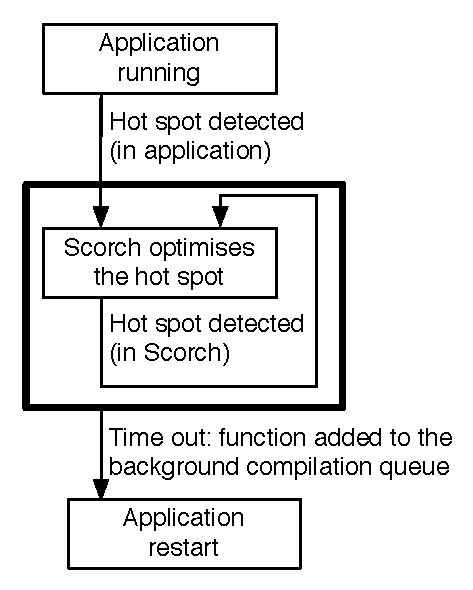
\includegraphics[width=0.4\linewidth]{InfiniteRecursionOptPbCritical}}
		\hfill
		\subfigure[Background mode]{\label{fig:InfiniteRecursionOptPbBackground}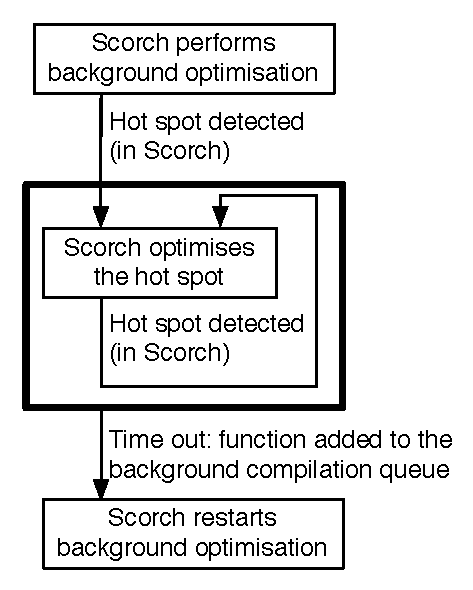
\includegraphics[width=0.4\linewidth]{InfiniteRecursionOptPbBackground}}
		\subfigure{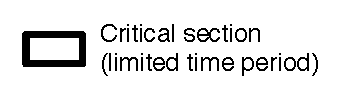
\includegraphics[width=0.3\linewidth]{InfiniteRecursionOptPbLegend}}
		\caption{Infinite recursion problem in the two optimisation modes}
    \end{center}
\end{figure}

%slow down - background
It can conceptually happen that the optimiser starts spinning while searching the stack for a function to optimise. In this case, no function can be added to the background compilation queue as the optimiser has not been able to find a function to optimise in the limited time period. In practice, in our case, the stack search code is quite simple and no hot spot can be detected repeatedly in this code.

When the application becomes idle, the optimiser is started in background mode to optimise functions in the background compilation queue. In this case, the optimiser always successfully generates and installs optimised functions. However, the optimisation of a function is verey slow. Indeed, while the optimiser is running in background mode, it activates itself in critical mode when detecting hot spots in its own code. Each time it happens, the optimiser spins in critical mode for the time period allowed as shown on figure \ref{fig:InfiniteRecursionOptPbBackground}. If the optimiser is started many times on itself during background optimisation, the optimisation of the function may take a significant amount of time. 

Eventually, the optimiser optimise most of its own code correctly through the background mode. Once done, both modes can work correctly as no hot spot can be detected in optimised code.

The problem is therefore that the application executed gets really slow at start-up because of time wasted spinning in critical mode. Peak performance takes a long time to reach because the optimiser successfully installs code only in background mode or when the infinite recursion issue does not happen in critical mode. 

\subsection{Current solution}

The first solution we wanted to implement was to disable the optimiser when it is running. This first design has a significant advantage: it is quite simple both conceptually and implementation-wise, while it completely avoids the infinite recursion problem. It has however a major drawback: the optimiser cannot optimise its own code any more. Of course, the optimiser may use core libraries that can be optimised. For example, the optimiser may use collections such as arrays. If the application optimised is also using the same collections, and it is very likely that an application would use arrays, the array code base may get optimised. Then, the optimiser ends up using an optimised version of arrays. For this reason, it is possible that while optimising code the optimiser triggers the deoptimiser, and it works perfectly fine.

%call-back removal / addition implementation
To implement our first solution, we changed the VM call-back activating the optimiser to uninstall itself upon activation. When a hot spot is detected but the call-back is not installed, the VM resets the profiling counters which has reached the hot spot threshold and restarts immediately the execution of the application. Then, we changed the optimiser to install back the call-back when it resumes the application, after adding a function to the background queue or installing optimised code. This way, we believed the optimiser would never end up in a situation where it optimises itself, solving entirely the problem.

%can optimise itself through back process
Then, we ran our benchmarks and saw that the problem was solved but the optimiser could still optimise its own code. Our first implementation effectively disabled the optimiser, but only when it was running on critical mode. When hot spots were detected, they were optimised or postponed without any issue as the optimiser disabled itself in critical mode, and the application resumed just fine. When the optimiser was started in background mode, it was not disabled. Hence, in this case, the optimiser was sometimes interrupted by itself in critical mode to get optimised.

%1st sol work and good enough 
This first solution is implemented, stable and works fine. Multiple benchmarks run with significant speed-up over the normal VM (This will be detailed in chapter \ref{chap:validation}). In general, in the production VM, simplicity is really important to keep the code base relatively easy to maintain. For each added complexity in the VM we wonder if the complexity is worth the benefit. This first solution is nice because it is simpler, both to understand and to maintain, than the alternative ones, so the optimising JIT may move to production with this design. Alternative solutions, more complex but with less constraints, are discussed in the next section.

\subsection{Discussion and advanced solutions}

%but cannot optimise itself in critical mode
The first solution is working but there is one major drawback: Scorch optimiser cannot optimise itself in critical mode. 

With the current solution, hot spots detected inside the optimiser in critical mode are completely ignored and the corresponding profiling counters are reset. If the optimiser attempts to inline code later, it may get confused by some counter values which were reset. The optimiser may speculate that a branch was not taken while in fact the branch was taken but the counters were reset. 

We could implement some kind of decay strategy instead of completely resetting the counters. We did not go in this direction because the counters are encoded in 16 bits while the hot spot threshold is at 60,000. Due to the 16 bits encoding limitation, not completely resetting the counters leads to many hot spot detected without anything happening, slowing down the optimiser code at start-up. Further analysis in this direction are required to conclude anything.

%the postpone pb while in critical mode - Saving current stack impossible
Based on advises from other people, we considered, instead of disabling the optimiser when it is running in critical mode, to postpone the optimisation to the background mode. In our design, it is quite difficult to do so. Indeed, when the VM call-back starts the optimiser, it provides only a reification of the current stack. The optimiser then needs to search the stack to select a function to optimise. As the stack is modified upon execution, it is not possible to save it efficiently so that the optimiser can search it later in the background green thread. As discussed in section \ref{ss:stackSearch}, there is no obvious cheap heuristic to figure out what function is the best to optimise based on the current stack (especially, picking the bottom frame function is usually not a good idea). It is however possible, once the optimiser has found what function to optimise, to add it to the background compilation queue. 

We believe that instead of disabling the entire optimiser while it is running in critical mode, we could instead disable it only during the stack searching phase in critical mode. The stack search phase represents less than 1\% of the optimiser execution time. The selected function optimisation may be postponed to the background green thread. This way, only hot spots detected during the stack search would be ignored, while the rest of the optimiser would be optimised at the next idle pause.

\paragraph{Ahead-of-time optimisation.} 
Alternatively, we could consider optimising the Scorch optimiser code ahead-of-time.

As the Sista architecture allows to persist optimised code (This is discussed in details in the following chapter), the optimiser code could be preheated through warm-up runs, for example by giving it a list of well-chosen functions to optimise. This way, all hot spots inside the optimiser would be detected ahead of time and optimised. The optimised optimiser code would be shipped to production.

Alternatively, the optimiser's code could be optimised statically by calling itself on its own code, using types inferred from a static type inferencer instead of types inferred from the runtime.

%\subsection{Dependencies and optimisations} 

% from 1 old part
%Rephrase -  solution does not forbig Scorch to use optimise libs

% maybe only one sentence ? -> be careful about dependencies
%The first constraint to note when programming Scorch, which may be obvious to the Kernel programmer, is that Scorch cannot depends on any framework or library but the Kernel and Core libraries. Each framework or library in the system relies on the execution engine to perform its code. Scorch is part of the execution engine. Hence, if Scorch relies on an external library and that someone modifies the library, the execution engine may not be stable any more and the runtime completely crashes. In fact, all the Kernel code and Core librairies have similar constraints, they cannot rely on anything to keep the system modular. 

%While writting Scorch, we needed a tool to compress the deoptimisation metadata generated aside from the optimised code. We wanted to use the standard Pharo serializer, Fuel (CITE), but we were not able to do it or further modification on Fuel would break the execution engine.

%In the end, we limited the dependencies of Scorch to the Pharo Kernel and the core collections (exactly: Set, OrderedCollection, Array, ByteArray and Dictionary in addition to the kernel). Any change on one of this dependency may require to change something in Scorch to keep the system running.


%\subsection{Debugging and runtime modification}

%Should I talk about that at all ? I was thinking over a restricted compiling to C but maybe we don't care.

%Maybe rewrite so that formally does not work but in practice it does.

%As any Smalltalk program, it is possible to modify the optimiser while it is running, for example in the debugger. If the modifications leads to incorrect optimiser behavior, then the runtime may crash. To avoid crashes, it may be wise to disable the optimiser while editing it. In practice, this feature is used only by the optimiser implementors. It is very useful to debug the optimiser to understand specific bugs or compiler decisions. With careful understanding of the infrastructure, it is possible in practice to debug the optimiser while it is running and modify its code. The optimiser is set by default to catch all exceptions, failing the optimisation of a specific v-function if an exception was raised. Hence, if the code modification triggers a compile-time exception, the system shall not crash. Unfortunately, in some cases, the optimiser may have silent errors, generating incorrect code without raising exceptions and completely crashing the system.

%The only part of Scorch that cannot really be edited is the deoptimisation metadata generation. Indeed, deoptimisation metadata is also used by the deoptimiser which, as detailled in the following section, has stronger constraints on its code. If one modifies the deoptimisation metadata generated, the deoptimiser may not be able to deoptimise correctly optimised code any more, leading to crashes.

%%%%%%%%%%%%%%%%%%%%%%%%%%%%%%%%%%%%%%%%%%%%%%%%%%%%%%%%%%%%%%%%%%%%%%%%%%%%%%%%%%%%%%%%%%%%%%%%%%%%%%%%%%%%%%%%%%%%%%%%%%%%%

%KEEP WRITING FROM HERE

\section{Scorch deoptimiser}

The deoptimiser can be activated in multiple situations. If an optimisation time assumption is invalid at runtime, a deoptimisation guard fails and Cogit triggers a call-back to deoptimise the stack. In addition, multiple development tools in the language, such as the debugging tools, may call the deoptimiser to introspect the stack.

\subsection{Infinite recursion issue}

% repeat problem for deopt
As Scorch deoptimiser is written in Smalltalk, its code base may get optimised. If one of the optimisation-time speculation is incorrect at runtime, the frame representing the execution of the optimised function requires the deoptimiser to restore the stack frames with non optimised functions to continue the execution of the program. In the case where the deoptimiser functions are optimised, the deoptimiser may call itself on one of its own frame to be able to continue deoptimising code. If each time the deoptimiser calls itself on one of its own frame, the deoptimisation cannot terminate because the deoptimiser needs to call itself again on of its own frame, the application gets stuck in an infinite loop.

Figure \ref{fig:InfiniteRecursionDeoptPb} shows the problem in the case where the deoptimiser is triggered by a guard failure. On the left, in the normal deoptimisation flow, the application is interrupted when a guard fails. The deoptimiser recreates the non optimised stack frames from the optimised stack frame and edits the stack. The application can then resume with non optimised code. On the right, in the infinite recursion issue, the application is also interrupted when a guard fails. However, while the deoptimiser is deoptimising the stack, another guard fails in the deoptimiser code. The deoptimiser then restarts to deoptimise one of its own frame, but another guard fails in its own code. The deoptimiser keeps restarting the deoptimisation of one of its own frame and the application gets stuck in an infinite loop.

\begin{figure}[h!]
    \begin{center}
        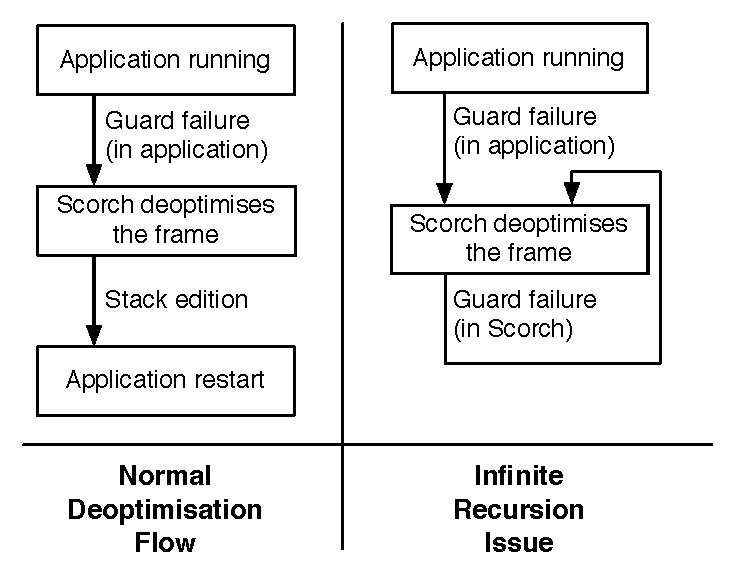
\includegraphics[width=0.65\linewidth]{InfiniteRecursionDeoptPb}
        \caption{Infinite recursion problem during deoptimisation}
        \label{fig:InfiniteRecursionDeoptPb}
    \end{center}
\end{figure}

This problem was solved in the optimiser by disabling it temporarily in specific circumstances. The optimiser could be disabled as the execution could simply fall back to non optimised code. The deoptimiser cannot however be disabled or any application green thread requiring deoptimisation would not be able to keep executing code. As the deoptimiser cannot be disabled, it is not possible to solve the infinite recursion problem in the same way than the optimiser. 

To solve this infinite recursion problem, we implemented two different solutions. The first solution attempts to restore the runtime in a "recovery mode" when recursive deoptimisation happens. In recovery mode, no optimised function can be used (the runtime relies entirely on the v-function interpreter and the baseline JIT). This solution was used for the first benchmarks, but it did not work correctly with benchmarks creating multiple green threads and making this solution thread-safe had too many constraints. We then designed and implemented a second solution in use now. The second solution consists in keeping all the deoptimiser code in a library completely independent from the rest of the system that cannot be optimised.

\subsection{Recovery mode}

As a first attempt to solve the infinite recursion issue for the deoptimiser, we forced Scorch to keep a recovery copy of each method dictionary where optimised v-functions are installed. The recovery copies include only non optimised v-functions. We added a global flag, marking if a deoptimisation is in progress. If the deoptimiser is activated while a deoptimisation is in progress (this can be known thanks to the global flag), the deoptimiser falls back to recovery mode. To do so, the deoptimiser use the primitive \ct{become:} to swap all method dictionaries with their recovery copy and disables the optimiser not to optimise anything in the recovery copies. The deoptimiser can then deoptimise the stack without calling itself repeatedly as it now uses only non optimised functions. Once the stack is deoptimised, the deoptimiser restores the method dictionaries with the optimised v-functions and re-enables the optimiser. 

With this solution, most of the deoptimiser code can be optimised as if an infinite recursion happens, the runtime switches to recovery mode and executes correctly the code. Only most of the deoptimiser code can be optimised as all the Smalltalk code executed from the guard failure call-back to the point where recovery mode is activated cannot be optimised. Such code is not protected by the recovery mode and may suffer from the infinite recursion issue. To avoid the problem, we marked a very small list of functions so they cannot be optimised.

We were able to run most benchmarks with this solutions. However, some benchmarks showed significant slow-down during deoptimisation. Moreover, other benchmarks (the ones using multiple green threads) were crashing. With this solution, we had two major problems. 

The first problem is that switching to recovery mode requires to edit many caches in the VM to use the non optimised version of functions. Each look-up cache entry referencing an optimised function needs to be edited to refer back to the non optimised function. Once the deoptimisation in recovery mode is terminated, the caches need to be updated again to reference the optimised functions. Updating all the caches can take a significant amount of time. Especially, in our implementation the inline caches are directly written in the native code and each mutation requires partial flush of the cpu instruction cache. The recovery mode therefore slowed down the application for a short while both due to the time spent for the VM to update the caches and for the cpu to restore all the instruction caches.

The second and main problem is that several of our benchmarks use multiple green threads. In this case, the global flag approach does not work as multiple deoptimisations may happen concurrently. One solution is to wrap the code switching from recovery mode to optimised mode and the other way around in semaphores to be green thread safe. However, every function called from the deoptimisation call-back to the point where recovery mode is enabled needs to be marked not to be optimised. We did not want to disable optimisations on code present in the semaphores and the process scheduler as such code may be performance critical in some applications. Forbidding the optimisation of such code seemed to be too restrictive. We concluded that this approach could not work for our production environment.

\subsection{Independent library}

As a second solution, we designed the whole deoptimiser as a completely independent Smalltalk library. The deoptimiser may use primitives but is not allowed to use any external functions. All the deoptimiser classes are marked: their functions do not have profiling counters and the Scorch optimiser is aware that the optimisation of such functions is not allowed. The deoptimiser code is therefore not optimised at runtime, it is running using only the v-function interpreter and the baseline JIT. As the deoptimiser code cannot be optimised and cannot use any external function that could be optimised, the infinite recursion issue cannot happen.

This solution has multiple important constraints. 

Firstly, the deoptimiser code cannot be optimised at runtime. This constraint is the least important as there are potential solutions. As deoptimisation is uncommon, arguably, not optimising the deoptimiser code is not a problem. In addition, this problem can be partially solved by optimising the deoptimiser code ahead-of-time using Scorch only with optimisations that do not require deoptimisation guards and type information inferred statically. As the library is quite small (500 LoC) and has a very strong invariant (it cannot call any external function), a type inferencer can be very precise and efficient.

Secondly, the deoptimiser code needs to be completely independent. Only primitives can be used directly because any external function may be optimised, potentially leading to the infinite recursion problem. We analysed what other libraires the deoptimiser depended on and remove most of the dependencies by duplicating a bit of code. However, the deoptimiser was relying both on arrays and dictionaries to deoptimise the stack. We create a minimal array and a minimal dictionary as part of the deoptimiser library. The two collection code have now to be maintained in parallel to the core collections.

Lastly, working of the deoptimiser is very tedious. A simple thing such as logging a string in the deoptimiser code require to call a function external to the deoptimiser and may lead to the infinite recursion problem.

Although the constraints are important, we were able to run all our benchmarks with this design. We believe we are going to keep this implementation to move to production.

%%%%%%%%%%%%%%%%%%%%%%%%%%%%%%%%%%%%%%%%%%%%%%%%%%%%%%%%%%%%%%%%%%%%%%%%%%%%%%%%%%%%%%%%%%%%%%%%%%%%%%%%%%%%%%%%%%%%%%%%%%%%%

\section{Related work}

To have an optimising JIT optimising its own code and encounter the infinite recursion problem we discussed in this chapter, the optimising JIT has to be written in one of the languages it can optimise and run in the same runtime than the optimised application. Such an optimising JIT is not common.

Many production VMs are entirely written in a low-level language such as C++ (CITE V8 Webkit hotspot). The optimising JIT cannot optimise its own code in such VMs. Other VMs such as the ones written with the RPython toolchain (CITE) are written in a language that the optimising JIT could optimise, but the production VMs are compiled ahead-of-time to native code, hence the optimising JIT does not optimise its own code at runtime in the production runtime. Some VMs are metacircular(CITE KLEIN and Jalapeno), which means they are entirely written in a language they can run. However, many metacircular VMs, such as Klein (CITE), do not feature an optimising JIT. 

Overall, there are two main VMs where the optimising JIT optimises its own code at runtime. On the one hand, there is the Graal compiler (CITE) which can be used both in the context of the Maxine VM (CITE) and the Java hotspot VM (CITE). The Graal compiler effectively optimises its own code at runtime as it would optimise the application code. On the other hand, Jikes RVM (CITE) features a runtime compiler that can optimise its own code at runtime. 

\subsection{Graal optimising JIT}

The Graal runtime compiler(CITE) was initially designed and implemented as part of the Maxine VM (CITE), a metacircular Java VM. Graal was then extracted from Maxine. It was then integrated in the Java hotspot VM (CITE). Graal can be used in two different ways on top of the hotspot VM. It can be used as an alternative optimising JIT, replacing the Java hotspot optimising JIT written in C++ or it can be used as a special purpose optimising JIT, optimising only specific libraries or application while the rest of the Java runtime is optimised with hotspot optimising JIT. VMs built with Truffle (CITE), a framework allowing to build efficient VMs by simply writting an AST interpreter in Java, are now running using the Java hotspot VM and the Graal compiler as the optimising JIT.

The most relevant use-case, in our context, is when the Graal compiler is used as an alternative optimising JIT on top of the Java hotspot VM. The interpreter and baseline JIT tiers are in this case present in Java hotspot VM, written in a low level language (C++) and compiled ahead-of-time to native code. In our case, the Pharo interpreter and baseline JIT are also compiled ahead-of-time to native code. The optimising JIT are in both cases written in the language run by the VM (Graal in Java and Scorch in Smalltalk), they can optimise their own code and they need to interface with the existing VM to trigger runtime compilation or to install optimised code.

In the Graal-hotspot runtime, when a hotspot is detected, code in the hotspot VM (written in C++) searches the stack for a function to optimise. Once the function is chosen, Hotspot adds it to a thread-safe compilation queue. The Graal compiler is run in different native threads concurrently to the application native threads. Graal takes functions to optimise from the compilation queue, generates concurrently optimised n-function and hands them over to the hotspot VM for installation. The optimised n-functions handed by Graal to hotspot respect the Graal Java native interface. They include deoptimisation metadata that hot spot is able to understand. When dynamic deoptimisation happens, code written in the hotspot VM (in C++) is responsible for the deoptimisation of the stack.

In our work, Scorch optimiser is able to optimise most of its own code unconditionnally, but the stack search code can be optimised only if the a hot spot is detected while the optimiser is running in background mode. Scorch deoptimiser code cannot be optimised at all. In the case of the Graal-hotspot runtime, the stack search and deoptimisation code is written in C++ and cannot be optimised by Graal. Having the stack search and deoptimisation code in Smalltalk, even if they cannot be optimised normally, allow us to change part of the design such as the deoptimisation metadata without having to recompile the VM. We therefore believe that our approach has an advantage over the Graal-hotspot runtime.

\subsection{Jikes RVM}

Jikes RVM (CITE) optimising runtime compiler is written entirely in Java and can optimise Java code. However, it is not currently able to use runtime information to direct its optimisations and do not generate deoptimisation guards, making it not that relevant in our context. The runtime compiler uses however an interesting technique (CITE ADAPTIVE) to choose what function to optimise. Jikes RVM uses an external sampling profiling native thread. Based on the profiling samples, the profiling thread detect what function should be optimised and adds it to a thread-safe compilation queue. The optimising runtime compiler can then start other native threads which take functions to optimise from the compilation queue, optimise and install them. 

The n-function generated by the Jikes RVM baseline JIT do not need profiling counters as profiling is performed using the samples taken by the profiling native thread. The functions to optimise are chosen entirely concurrently. The application is not interrupted, at any time, to search the stack for a function to optimise or to detect a hot spot.

We did not investigate in this direction because our VM is currently single threaded. We do not think it is possible to implement something similar in a single-threaded environment.

%%%%%%%%%%%%%%%%%%%%%%%%%%%%%%%%%%%%%%%%%%%%%%%%%%%%%%%%%%%%%%%%%%%%%%%%%%%%%%%%%%%%%%%%%%%%%%%%%%%%%%%%%%%%%%%%%%%%%%%%%%%%%

\section{Conclusion}

In this chapter we discussed the main issue existing because the optimiser and the deoptimiser are implemented in Smalltalk and are running in the same runtime and the same native thread than the application they optimise and deoptimise respectively. The main issue is related to infinite recursion. If a hot spot is detected inside the optimiser code, the optimiser may call itself indefinitely to try to optimise it. The deoptimiser has a similar issue when it needs to deoptimise its own code. In both cases, the program may get slow or gets completely stuck.

The optimiser solves this issue by disabling itself when it runs in critical mode (when it interrupts temporarily the application green thread to perform the optimisation). The optimiser cannot optimise itself directly while running in critical mode, it can only optimise the  application, which may include libraries used both by the application and the optimiser itself. For functions taking a long time to optimise, the optimiser cannot stop the application for too long or the application becomes unresponsive, hence it postpone the optimisation to a background compilation queue where functions are optimised when the application is in idle. When performing optimisations in the background, the optimiser can optimise itself entirely.

The deoptimiser cannot solve the problem the same way as it cannot be disabled at any time or Smalltalk code cannot be executed any more. The deoptimiser avoids the problem by being written using a small number of classes that cannot be optimised nor call any other libraries.

The next chapter explains how the runtime state is persisted across multiple VM start-ups, including the running green threads and the optimised functions.

\ifx\wholebook\relax\else
    \end{document}
\fi
\ifx\wholebook\relax\else

% --------------------------------------------
% Lulu:

    \documentclass[a4paper,12pt,twoside]{../includes/ThesisStyle}

	\usepackage[T1]{fontenc} %%%key to get copy and paste for the code!
%\usepackage[utf8]{inputenc} %%% to support copy and paste with accents for frnehc stuff
\usepackage{times}
\usepackage{ifthen}
\usepackage{xspace}
\usepackage{alltt}
\usepackage{latexsym}
\usepackage{url}            
\usepackage{amssymb}
\usepackage{amsfonts}
\usepackage{amsmath}
\usepackage{stmaryrd}
\usepackage{enumerate}
\usepackage{cite}
%\usepackage[pdftex,colorlinks=true,pdfstartview=FitV,linkcolor=blue,citecolor=blue,urlcolor=blue]{hyperref}
\usepackage{xspace}
%\usepackage{graphicx}
\usepackage{subfigure}
\usepackage[scaled=0.85]{helvet}
        
        
\newcommand{\sepe}{\mbox{>>}}
\newcommand{\pack}[1]{\emph{#1}}
\newcommand{\ozo}{\textsc{oZone}\xspace}
\newcommand\currentissues{\par\smallskip\textbf{Current Issues -- }}

\newboolean{showcomments}
\setboolean{showcomments}{true}
\ifthenelse{\boolean{showcomments}}
  {\newcommand{\bnote}[2]{
	\fbox{\bfseries\sffamily\scriptsize#1}
    {\sf\small$\blacktriangleright$\textit{#2}$\blacktriangleleft$}
    % \marginpar{\fbox{\bfseries\sffamily#1}}
   }
   \newcommand{\cvsversion}{\emph{\scriptsize$-$Id: macros.tex,v 1.1.1.1 2007/02/28 13:43:36 bergel Exp $-$}}
  }
  {\newcommand{\bnote}[2]{}
   \newcommand{\cvsversion}{}
  } 


\newcommand{\here}{\bnote{***}{CONTINUE HERE}}
\newcommand{\nb}[1]{\bnote{NB}{#1}}
\newcommand{\fix}[1]{\bnote{FIX}{#1}}
%%%% add your own macros 

\newcommand{\sd}[1]{\bnote{Stef}{#1}}
\newcommand{\ja}[1]{\bnote{Jannik}{#1}}
\newcommand{\na}[1]{\bnote{Nico}{#1}}
%%% 


\newcommand{\figref}[1]{Figure~\ref{fig:#1}}
\newcommand{\figlabel}[1]{\label{fig:#1}}
\newcommand{\tabref}[1]{Table~\ref{tab:#1}}
\newcommand{\layout}[1]{#1}
\newcommand{\commented}[1]{}
\newcommand{\secref}[1]{Section \ref{sec:#1}}
\newcommand{\seclabel}[1]{\label{sec:#1}}

%\newcommand{\ct}[1]{\textsf{#1}}
\newcommand{\stCode}[1]{\textsf{#1}}
\newcommand{\stMethod}[1]{\textsf{#1}}
\newcommand{\sep}{\texttt{>>}\xspace}
\newcommand{\stAssoc}{\texttt{->}\xspace}

\newcommand{\stBar}{$\mid$}
\newcommand{\stSelector}{$\gg$}
\newcommand{\ret}{\^{}}
\newcommand{\msup}{$>$}
%\newcommand{\ret}{$\uparrow$\xspace}

\newcommand{\myparagraph}[1]{\noindent\textbf{#1.}}
\newcommand{\eg}{\emph{e.g.,}\xspace}
\newcommand{\ie}{\emph{i.e.,}\xspace}
\newcommand{\ct}[1]{{\textsf{#1}}\xspace}


\newenvironment{code}
    {\begin{alltt}\sffamily}
    {\end{alltt}\normalsize}

\newcommand{\defaultScale}{0.55}
\newcommand{\pic}[3]{
   \begin{figure}[h]
   \begin{center}
   \includegraphics[scale=\defaultScale]{#1}
   \caption{#2}
   \label{#3}
   \end{center}
   \end{figure}
}

\newcommand{\twocolumnpic}[3]{
   \begin{figure*}[!ht]
   \begin{center}
   \includegraphics[scale=\defaultScale]{#1}
   \caption{#2}
   \label{#3}
   \end{center}
   \end{figure*}}

\newcommand{\infe}{$<$}
\newcommand{\supe}{$\rightarrow$\xspace}
\newcommand{\di}{$\gg$\xspace}
\newcommand{\adhoc}{\textit{ad-hoc}\xspace}

\usepackage{url}            
\makeatletter
\def\url@leostyle{%
  \@ifundefined{selectfont}{\def\UrlFont{\sf}}{\def\UrlFont{\small\sffamily}}}
\makeatother
% Now actually use the newly defined style.
\urlstyle{leo}



	\usepackage{amsmath,amssymb}             % AMS Math
% \usepackage[french]{babel}
\usepackage[latin1]{inputenc}
\usepackage[T1]{fontenc}
\usepackage[left=1.5in,right=1.3in,top=1.1in,bottom=1.1in,includefoot,includehead,headheight=13.6pt]{geometry}
\renewcommand{\baselinestretch}{1.05}

\usepackage{multicol}

% Table of contents for each chapter

\usepackage[nottoc, notlof, notlot]{tocbibind}
\usepackage{minitoc}
\setcounter{minitocdepth}{1}
\mtcindent=15pt
% Use \minitoc where to put a table of contents

\usepackage{enumitem}

\usepackage{aecompl}

% Glossary / list of abbreviations

%\usepackage[intoc]{nomencl}
%\renewcommand{\nomname}{List of Abbreviations}
%
%\makenomenclature

% My pdf code

\usepackage[pdftex]{graphicx}
\usepackage[a4paper,pagebackref,hyperindex=true]{hyperref}

\usepackage{pgfplotstable,booktabs,colortbl}
\pgfplotsset{compat=1.8}

% Links in pdf
\usepackage{color}
\definecolor{linkcol}{rgb}{0,0,0.4} 
\definecolor{citecol}{rgb}{0.5,0,0} 

% Change this to change the informations included in the pdf file

% See hyperref documentation for information on those parameters

\hypersetup
{
bookmarksopen=true,
pdftitle="Sista: a Metacircular Architecture for Runtime Optimisation Persistence",
pdfauthor="Clement BERA", 
pdfsubject="Thesis", %subject of the document
%pdftoolbar=false, % toolbar hidden
pdfmenubar=true, %menubar shown
pdfhighlight=/O, %effect of clicking on a link
colorlinks=true, %couleurs sur les liens hypertextes
pdfpagemode=None, %aucun mode de page
pdfpagelayout=SinglePage, %ouverture en simple page
pdffitwindow=true, %pages ouvertes entierement dans toute la fenetre
linkcolor=linkcol, %couleur des liens hypertextes internes
citecolor=citecol, %couleur des liens pour les citations
urlcolor=linkcol %couleur des liens pour les url
}

% definitions.
% -------------------

\setcounter{secnumdepth}{3}
\setcounter{tocdepth}{1}

% Some useful commands and shortcut for maths:  partial derivative and stuff

\newcommand{\pd}[2]{\frac{\partial #1}{\partial #2}}
\def\abs{\operatorname{abs}}
\def\argmax{\operatornamewithlimits{arg\,max}}
\def\argmin{\operatornamewithlimits{arg\,min}}
\def\diag{\operatorname{Diag}}
\newcommand{\eqRef}[1]{(\ref{#1})}

\usepackage{rotating}                    % Sideways of figures & tables
%\usepackage{bibunits}
%\usepackage[sectionbib]{chapterbib}          % Cross-reference package (Natural BiB)
%\usepackage{natbib}                  % Put References at the end of each chapter
                                         % Do not put 'sectionbib' option here.
                                         % Sectionbib option in 'natbib' will do.
\usepackage{fancyhdr}                    % Fancy Header and Footer

% \usepackage{txfonts}                     % Public Times New Roman text & math font
  
%%% Fancy Header %%%%%%%%%%%%%%%%%%%%%%%%%%%%%%%%%%%%%%%%%%%%%%%%%%%%%%%%%%%%%%%%%%
% Fancy Header Style Options

\pagestyle{fancy}                       % Sets fancy header and footer
\fancyfoot{}                            % Delete current footer settings

%\renewcommand{\chaptermark}[1]{         % Lower Case Chapter marker style
%  \markboth{\chaptername\ \thechapter.\ #1}}{}} %

%\renewcommand{\sectionmark}[1]{         % Lower case Section marker style
%  \markright{\thesection.\ #1}}         %

\fancyhead[LE,RO]{\bfseries\thepage}    % Page number (boldface) in left on even
% pages and right on odd pages
\fancyhead[RE]{\bfseries\nouppercase{\leftmark}}      % Chapter in the right on even pages
\fancyhead[LO]{\bfseries\nouppercase{\rightmark}}     % Section in the left on odd pages

\let\headruleORIG\headrule
\renewcommand{\headrule}{\color{black} \headruleORIG}
\renewcommand{\headrulewidth}{1.0pt}
\usepackage{colortbl}
\arrayrulecolor{black}

\fancypagestyle{plain}{
  \fancyhead{}
  \fancyfoot{}
  \renewcommand{\headrulewidth}{0pt}
}

\usepackage{algorithm}
\usepackage[noend]{algorithmic}

%%% Clear Header %%%%%%%%%%%%%%%%%%%%%%%%%%%%%%%%%%%%%%%%%%%%%%%%%%%%%%%%%%%%%%%%%%
% Clear Header Style on the Last Empty Odd pages
\makeatletter

\def\cleardoublepage{\clearpage\if@twoside \ifodd\c@page\else%
  \hbox{}%
  \thispagestyle{empty}%              % Empty header styles
  \newpage%
  \if@twocolumn\hbox{}\newpage\fi\fi\fi}

\makeatother
 
%%%%%%%%%%%%%%%%%%%%%%%%%%%%%%%%%%%%%%%%%%%%%%%%%%%%%%%%%%%%%%%%%%%%%%%%%%%%%%% 
% Prints your review date and 'Draft Version' (From Josullvn, CS, CMU)
\newcommand{\reviewtimetoday}[2]{\special{!userdict begin
    /bop-hook{gsave 20 710 translate 45 rotate 0.8 setgray
      /Times-Roman findfont 12 scalefont setfont 0 0   moveto (#1) show
      0 -12 moveto (#2) show grestore}def end}}
% You can turn on or off this option.
% \reviewtimetoday{\today}{Draft Version}
%%%%%%%%%%%%%%%%%%%%%%%%%%%%%%%%%%%%%%%%%%%%%%%%%%%%%%%%%%%%%%%%%%%%%%%%%%%%%%% 

\newenvironment{maxime}[1]
{
\vspace*{0cm}
\hfill
\begin{minipage}{0.5\textwidth}%
%\rule[0.5ex]{\textwidth}{0.1mm}\\%
\hrulefill $\:$ {\bf #1}\\
%\vspace*{-0.25cm}
\it 
}%
{%

\hrulefill
\vspace*{0.5cm}%
\end{minipage}
}

\let\minitocORIG\minitoc
\renewcommand{\minitoc}{\minitocORIG \vspace{1.5em}}

\usepackage{multirow}
\usepackage{slashbox}

\newenvironment{bulletList}%
{ \begin{list}%
	{$\bullet$}%
	{\setlength{\labelwidth}{25pt}%
	 \setlength{\leftmargin}{30pt}%
	 \setlength{\itemsep}{\parsep}}}%
{ \end{list} }

\newtheorem{definition}{D�finition}
\renewcommand{\epsilon}{\varepsilon}

% centered page environment

\newenvironment{vcenterpage}
{\newpage\vspace*{\fill}\thispagestyle{empty}\renewcommand{\headrulewidth}{0pt}}
{\vspace*{\fill}}



	\graphicspath{{.}{../figures/}}
	\begin{document}
\fi

\chapter{Runtime state persistance across start-ups}
\label{chap:persistance}
\minitoc

TODO: sec1,sec3,sec4 add papers from review in conf

This chapter describes how the Sista VM persists the runtime state across multiple VM start-ups, including the running green threads and the optimised code. The first section discusses how snapshots are implemented in Smalltalk, including how the code and the running green threads are persisted across start-ups. Section \ref{sec:warmup} focuses on the main issue: the start-up performance of many VMs today is far worse than the peak performance. Several cases where the start-up performance is a problem are described. Section \ref{sec:persistanceSol} details our solution: optimised v-functions are persisted across multiple start-ups, allowing to persist optimised code and the running green threads. Section \ref{sec:relWork} compares our approach to existing VMs. Few VMs attempts to persist the runtime state across multiple start-ups, but some VMs include solutions to improve start-up performance, solving the same problem of poor start-up performance.

\section{Snapshots and persistance}

- discuss snapshots again. 
and persist v-function, 
Explain briefly cogit mapping and v-function persistance.
Explain saving processes
platform independent
Restart from snapshot and move from v-function interpretation to n-func in loop and function call.

TO CHECK


In the Smalltalk terminology, a snapshot, also called \emph{image}, is a sequence of bytes that represents a serialized form of all the objects present at a precise moment in the runtime. As everything is an object in Smalltalk, including processes, the virtual machine can, at start-up, load all the objects from a snapshot and resume the execution based on the active process precised by the snapshot. In fact, this is the normal way of launching a Smalltalk runtime. 

In Dart, the word snapshot refers to the serialized form of one or more Dart objects \cite{Anna13a}. Dart snapshots can save the whole heap, as part of their \emph{full snapshots}, but as far as we know it is not possible in this language to save processes. Hence, the virtual machine always restarts at the \ct{main} function once the snapshot is loaded.

One interesting problem in snapshots is how to save the call stack, \ie the processes. It possible in the Smalltalk virtual machine to convert each stack frame to a context object reifying the function activation. To perform a snapshot, each stack frame is reified and only objects are saved in the snapshot. When the snapshot is restarted, the virtual machine recreates a stack frame for each function activation lazily from the context objects. 

TOCHECK


To avoid this warm-up time, this paper introduces an architecture to save a platform-independent version of the optimized code as part of a snapshot. Snapshots are available in multiple object-oriented languages such as Smalltalk \cite{Gold83a} and later Dart \cite{Anna13a}. Snapshots allow the program to save the heap in a given state, and the virtual machine can resume execution from this snapshot later. Usually, compiled code is available in different versions. On the one hand, a bytecoded version, which is on the heap if the bytecoded version of functions is reified as an object (as in Dart and Smalltalk).  On the other hand one or several machine code versions are available in the machine code zone. Machine code versions are usually not part of the heap directly but of a separated part of memory which is marked as executable. Snapshots cannot save easily machine code versions of functions as a snapshot needs to be platform-independent and machine code versions of functions are not regular objects.

END TO CHECK

\section{Warm-up time problem}
\label{sec:warmup}

The most important problem we attempt to solve by persisting the runtime state across start-up is the warm-up time problem, i.e., the time wasted by the VM at each start-up to reach peak performance. Depending on use-cases, the warm-up time may not matter. The warm-up time required to reach peak performance may be negligible compared to the overall runtime of the application. However, when applications are started frequently and are short-lived, this time can matter.

We give three examples where the virtual machine start-up time matters. These examples are specific, but they give an idea where the warm-up performance is a serious problem.

\paragraph{Distributed applications.}
Modern large distributed applications run on hundreds, if not thousands, of machines such as the slaves one can rent on Amazon Web Services. Slaves are usually rented per hour, though now some contracts allow one to rent a slave for 5 minutes or even 30 seconds. If the application needs more power, it rents new slaves, if it does not need it anymore, it frees the slaves. The slaves are paid only when needed, no application users imply no cost whereas the application can scale very well.

The problem is that to reduce the cost to the minimum, the best would be to rent a slave when needed, and at the second where the slave is not used, to free it not to pay anymore for it. Doing that implies having very short lived slaves, with an order of 30 seconds life-time for example. To be worth it, the time between the slave start-up and the peak performance of the language used has to be as small as possible. A good VM for such kind of scenario should reach peak performance very fast.

\paragraph{Mobile application.}
In the case of mobile applications, the start-up performance matters because of  battery consumption. During warm-up time, the optimizing compiler recompiles frequently used code. All this compilation process requires time and energy, whereas the application is not run. In the example of the Android runtime, the implementation used JIT compilation with the Dalvik VM \cite{Born08a}, then switched to client-side ahead of time compilation (ART) to avoid that energy consumption at start-up, and is now switching back to JIT compilation because of the AOT (Ahead of Time compiler) constraints \cite{Geof15a}. These different attempts show the difficulty to build a system that requires JIT compilation for high performance but can't afford an energy consuming start-up time.

\paragraph{Web pages.}
Web pages sometimes execute just a bit of Javascript code at start-up, or use extensively Javascript in their lifetime (in this latter case, one usually talk about web application). A Javascript virtual machine has to reach peak performance as quickly as possible to perform well on web pages where only a bit of Javascript code is executed at start-up, while it has also to perform well on long running web applications.

\section{Persistance of optimised virtual functions}
\label{sec:persistanceSol}

- Solution snapshot optimised v-functions - work the same way.
platform independent, moving from v-func interpretation to n-function.
Discussion on reg alloc and Cogit compilation time.

TO CHECK


Our architecture, \emph{Sista} (Speculative Inlining SmallTalk Architecture) works as follows. Our optimizing compiler, after doing language-specific optimizations such as speculative inlining or array bounds check elimination, generates an optimized version of the function using a bytecode representation and does not directly generate machine code. This optimized version has access to an extended bytecode set to encode unchecked operations such as array access without bounds checks similar to the work of B\'era et al.\cite{Bera14a}. Optimized bytecoded functions are reifed as objects the same as normal bytecoded functions, hence they can be saved without any additional work as part of the snapshot. Then, the VM uses the baseline Just-in-Time compiler (JIT) as a back-end to generate machine code from the optimized bytecoded function. The optimized functions are marked, so the VM can decide to handle differently optimized bytecoded functions. 

Dynamic deoptimization is also split in two steps. Firstly, Sista asks the baseline JIT to reify the stack frame from machine state to bytecode interpreter state of the optimized bytecoded function, mapping correctly the register to stack entries and converting object representations from unboxed versions to boxed versions, as it would do for any unoptimized version of the function. Secondly, a separate deoptimizer maps the bytecode interpreter state of the optimized bytecoded function to multiple stack frame corresponding to the bytecode interpreter state of multiple unoptimized functions, rematerializing objects from constants and stack values.

With this architecture, the Sista VM can reach peak performance almost immediately after start-up if it starts from a snapshot where optimized code was persisted.

TO CHECK


We solve this warm-up time problem by saving runtime optimizations across start-ups. This way, we are able to start the virtual machine in a pre-heated state. With this approach, we reuse and take advantage of techniques reaching peak performance but with the advantage of being effective without warm-up time. 

\paragraph{Platform-independent.}We save optimizations across start-ups in a platform-independent way: this implies that we cannot save directly machine code. As our technique depends on snapshots, the platform-dependency depends on the snapshot being dependent on a platform or not. 

\paragraph{Bytecode saved.}Our approach saves the optimized code as a bytecoded version because the languages with snapshots already supports saving bytecoded functions as part of the snapshot. Bytecode is already a compressed and platform-independent representation of executable code. The optimized code is saved using an extended bytecode set to encode unchecked operations. %\sd{However, we believe that our approach is not exclusively tight with snapshots but could be used with a system serialising bytecodes.} \md{the problem is that then the whole point of the paper is a bit weak... I would maybe discuss it in the discussion section} 

\paragraph{Simplicity.}We try to keep the solution simple by reusing the existing snapshot infrastructure, which can persist the bytecode version of each methods. We do not want to extend the snapshot logic to be able to persist machine code as it is very complex. More precisely, we would need to extend the snapshot logic with specific code for each back-end supported (currently at least ARMv5, x86, x64 and MIPS little endian) and we would need to handle cases such as position-dependent machine code.


\section{Related work}
\label{sec:relWork}

\emph{TO DO: add the ones from author review.
+ from review of author}

This section discusses other strategies implemented in other VMs and research projects to decrease the warm-up time.

\subsection{Preheating through snapshots in Dart}

The Dart programming languages features snapshots for fast application start-up. In Dart, the programmer can generate different kind of snapshots \cite{Anna13a}. Since that publication, the Dart team have added two new kind of snapshots, specialized for iOS and Android application deployment, which are the most similar to our snapshots.

\paragraph{Android.} A Dart snapshot for an Android application is a complete representation of the application code and the heap once the application code has been loaded but before the execution of the application. The Android snapshots are taken after a warm-up phase to be able to record call site caches in the snapshot. The call site cache is a regular heap object accessed from machine code, and its presence in the snapshot allows to persist type feedback and call site frequency.

In this case, the code is loaded pre-optimized with inline caches prefilled values. However, optimized functions are not loaded as our architecture allows to do. Only unoptimized code with precomputed runtime information is loaded.

\paragraph{iOS.} For iOS, the Dart snapshot is slightly different as iOS does not allow JIT compilers. All reachable functions from the iOS application are compiled ahead of time, using only the features of the Dart optimizing compiler that don't require dynamic deoptimization. A shared library is generated, including all the instructions, and a snapshot that includes all the classes, functions, literal pools, call site caches, etc.

This second case is difficult to compare to our architecture: iOS forbids machine code generation, which is currently required by our architecture. A good application of our architecture to iOS is future work.

\subsection{Fast warm-up}

An alternative to snapshots is to improve the JIT compiler so the peak performance can be reached as early as possible. The improvements would consists of decreasing the JIT compilation time by improving the efficiency of the JIT code, or have better heuristic so the JIT can generate optimized code with the correct speculations with little runtime information.

\paragraph{Tiered architecture}
One solution, used the Webkit VM\cite{Webkit15}, is to have a tiered architecture with many tiers. In the version of Webkit in production from March 2015 to February 2016 \cite{Webkit15}, the code is:
\begin{itemize}
\item interpreted by a bytecode interpreter the first 6 executions.
\item compiled to machine code at 7th execution, with a non optimizing compiler, and executed as machine code up to 66 executions.
\item recompiled to more optimized machine code at 67th execution, with an optimizing compiler doing some but not all optimizations, up to 666 executions.
\item recompiled to heavily optimized machine code at 667th execution, with an optimizing compiler using LLVM as a backend.
\end{itemize}

At each step, the compilation time is greater but the execution time decreases. This tiered approach (4 tiers in the case of Webkit), allows to have good performance from start-up, while reaching high performance for long running code. This kind of approaches has also draw-backs: the VM development team needs to maintain and evolve four different tiers.

\paragraph{Saving metadata.}

To reach quickly peak performance, an alternative of saving optimized code is to save the runtime information. The Dart snapshot saves already the call site information in its Android snapshots. Other techniques are available.

In Strongtalk \cite{Sun06}, a high-performance Smalltalk, it is possible to save the inlining decision of the optimizing compiler in a separate file. The optimizing compiler can then reuse this file to make the right inlining decision the first time a hot spot is detected.

\paragraph{Saving machine code.}

In the Azul VM Zing \cite{Azul}, available for Java, the official web site claims that "operations teams can save accumulated optimizations from one day or set of market conditions for later reuse" thanks to the technology called \emph{Ready Now!}. In addition, the website precises that the Azul VM provides an API for the developer to help the JIT to make the right optimization decisions. As Azul is closed source, implementation details are not entirely known. 

However, word has been that the Azul VM reduces the warm-up time by saving machine code across multiple start-ups. If the application is started on another processor, then the saved machine code is simply discarded. We did not go in this direction to persist the optimization in a platform-independent way (in our architecture, starting the application on x86 instead of ARMv5 does not require the saved optimized code to be discarded), but we have a small overhead due to the bytecode to machine code translation at each start-up. In addition, we believe it's very difficult to persist correctly machine code compared to persisting bytecodes.

\paragraph{Ahead-of-time compilation.}

The last alternative is to pre-optimize the code ahead of time. This can be done by doing static analysis over the code to try to infer types. Applications for the iPhone are a good example where static analysis is used to pre-optimize the Objective-C application. The peak performance is lower than with a JIT compiler if the program uses a lot of virtual calls, as static analysis are not as precised as runtime information on highly dynamic language. 
However, if the program uses few dynamic features (for example most of the calls are not virtual) and is running on top of a high-performance language kernel like the Objective-C kernel, the result can be satisfying.

\section{Conclusion.} This chapter discusses how the runtime state is persisted across multiple start-ups, improving the performance during start-up. The next chapter validates the Sista architecture, mainly through performance evaluation in a set of benchmarks. The validation chapter also evaluates the Sista VM performance when the runtime state is persisted across multiple start-ups.

\ifx\wholebook\relax\else
    \end{document}
\fi
%\ifx\wholebook\relax\else

% --------------------------------------------
% Lulu:

    \documentclass[a4paper,12pt,twoside]{../includes/ThesisStyle}

	\usepackage[T1]{fontenc} %%%key to get copy and paste for the code!
%\usepackage[utf8]{inputenc} %%% to support copy and paste with accents for frnehc stuff
\usepackage{times}
\usepackage{ifthen}
\usepackage{xspace}
\usepackage{alltt}
\usepackage{latexsym}
\usepackage{url}            
\usepackage{amssymb}
\usepackage{amsfonts}
\usepackage{amsmath}
\usepackage{stmaryrd}
\usepackage{enumerate}
\usepackage{cite}
%\usepackage[pdftex,colorlinks=true,pdfstartview=FitV,linkcolor=blue,citecolor=blue,urlcolor=blue]{hyperref}
\usepackage{xspace}
%\usepackage{graphicx}
\usepackage{subfigure}
\usepackage[scaled=0.85]{helvet}
        
        
\newcommand{\sepe}{\mbox{>>}}
\newcommand{\pack}[1]{\emph{#1}}
\newcommand{\ozo}{\textsc{oZone}\xspace}
\newcommand\currentissues{\par\smallskip\textbf{Current Issues -- }}

\newboolean{showcomments}
\setboolean{showcomments}{true}
\ifthenelse{\boolean{showcomments}}
  {\newcommand{\bnote}[2]{
	\fbox{\bfseries\sffamily\scriptsize#1}
    {\sf\small$\blacktriangleright$\textit{#2}$\blacktriangleleft$}
    % \marginpar{\fbox{\bfseries\sffamily#1}}
   }
   \newcommand{\cvsversion}{\emph{\scriptsize$-$Id: macros.tex,v 1.1.1.1 2007/02/28 13:43:36 bergel Exp $-$}}
  }
  {\newcommand{\bnote}[2]{}
   \newcommand{\cvsversion}{}
  } 


\newcommand{\here}{\bnote{***}{CONTINUE HERE}}
\newcommand{\nb}[1]{\bnote{NB}{#1}}
\newcommand{\fix}[1]{\bnote{FIX}{#1}}
%%%% add your own macros 

\newcommand{\sd}[1]{\bnote{Stef}{#1}}
\newcommand{\ja}[1]{\bnote{Jannik}{#1}}
\newcommand{\na}[1]{\bnote{Nico}{#1}}
%%% 


\newcommand{\figref}[1]{Figure~\ref{fig:#1}}
\newcommand{\figlabel}[1]{\label{fig:#1}}
\newcommand{\tabref}[1]{Table~\ref{tab:#1}}
\newcommand{\layout}[1]{#1}
\newcommand{\commented}[1]{}
\newcommand{\secref}[1]{Section \ref{sec:#1}}
\newcommand{\seclabel}[1]{\label{sec:#1}}

%\newcommand{\ct}[1]{\textsf{#1}}
\newcommand{\stCode}[1]{\textsf{#1}}
\newcommand{\stMethod}[1]{\textsf{#1}}
\newcommand{\sep}{\texttt{>>}\xspace}
\newcommand{\stAssoc}{\texttt{->}\xspace}

\newcommand{\stBar}{$\mid$}
\newcommand{\stSelector}{$\gg$}
\newcommand{\ret}{\^{}}
\newcommand{\msup}{$>$}
%\newcommand{\ret}{$\uparrow$\xspace}

\newcommand{\myparagraph}[1]{\noindent\textbf{#1.}}
\newcommand{\eg}{\emph{e.g.,}\xspace}
\newcommand{\ie}{\emph{i.e.,}\xspace}
\newcommand{\ct}[1]{{\textsf{#1}}\xspace}


\newenvironment{code}
    {\begin{alltt}\sffamily}
    {\end{alltt}\normalsize}

\newcommand{\defaultScale}{0.55}
\newcommand{\pic}[3]{
   \begin{figure}[h]
   \begin{center}
   \includegraphics[scale=\defaultScale]{#1}
   \caption{#2}
   \label{#3}
   \end{center}
   \end{figure}
}

\newcommand{\twocolumnpic}[3]{
   \begin{figure*}[!ht]
   \begin{center}
   \includegraphics[scale=\defaultScale]{#1}
   \caption{#2}
   \label{#3}
   \end{center}
   \end{figure*}}

\newcommand{\infe}{$<$}
\newcommand{\supe}{$\rightarrow$\xspace}
\newcommand{\di}{$\gg$\xspace}
\newcommand{\adhoc}{\textit{ad-hoc}\xspace}

\usepackage{url}            
\makeatletter
\def\url@leostyle{%
  \@ifundefined{selectfont}{\def\UrlFont{\sf}}{\def\UrlFont{\small\sffamily}}}
\makeatother
% Now actually use the newly defined style.
\urlstyle{leo}



	\usepackage{amsmath,amssymb}             % AMS Math
% \usepackage[french]{babel}
\usepackage[latin1]{inputenc}
\usepackage[T1]{fontenc}
\usepackage[left=1.5in,right=1.3in,top=1.1in,bottom=1.1in,includefoot,includehead,headheight=13.6pt]{geometry}
\renewcommand{\baselinestretch}{1.05}

\usepackage{multicol}

% Table of contents for each chapter

\usepackage[nottoc, notlof, notlot]{tocbibind}
\usepackage{minitoc}
\setcounter{minitocdepth}{1}
\mtcindent=15pt
% Use \minitoc where to put a table of contents

\usepackage{enumitem}

\usepackage{aecompl}

% Glossary / list of abbreviations

%\usepackage[intoc]{nomencl}
%\renewcommand{\nomname}{List of Abbreviations}
%
%\makenomenclature

% My pdf code

\usepackage[pdftex]{graphicx}
\usepackage[a4paper,pagebackref,hyperindex=true]{hyperref}

\usepackage{pgfplotstable,booktabs,colortbl}
\pgfplotsset{compat=1.8}

% Links in pdf
\usepackage{color}
\definecolor{linkcol}{rgb}{0,0,0.4} 
\definecolor{citecol}{rgb}{0.5,0,0} 

% Change this to change the informations included in the pdf file

% See hyperref documentation for information on those parameters

\hypersetup
{
bookmarksopen=true,
pdftitle="Sista: a Metacircular Architecture for Runtime Optimisation Persistence",
pdfauthor="Clement BERA", 
pdfsubject="Thesis", %subject of the document
%pdftoolbar=false, % toolbar hidden
pdfmenubar=true, %menubar shown
pdfhighlight=/O, %effect of clicking on a link
colorlinks=true, %couleurs sur les liens hypertextes
pdfpagemode=None, %aucun mode de page
pdfpagelayout=SinglePage, %ouverture en simple page
pdffitwindow=true, %pages ouvertes entierement dans toute la fenetre
linkcolor=linkcol, %couleur des liens hypertextes internes
citecolor=citecol, %couleur des liens pour les citations
urlcolor=linkcol %couleur des liens pour les url
}

% definitions.
% -------------------

\setcounter{secnumdepth}{3}
\setcounter{tocdepth}{1}

% Some useful commands and shortcut for maths:  partial derivative and stuff

\newcommand{\pd}[2]{\frac{\partial #1}{\partial #2}}
\def\abs{\operatorname{abs}}
\def\argmax{\operatornamewithlimits{arg\,max}}
\def\argmin{\operatornamewithlimits{arg\,min}}
\def\diag{\operatorname{Diag}}
\newcommand{\eqRef}[1]{(\ref{#1})}

\usepackage{rotating}                    % Sideways of figures & tables
%\usepackage{bibunits}
%\usepackage[sectionbib]{chapterbib}          % Cross-reference package (Natural BiB)
%\usepackage{natbib}                  % Put References at the end of each chapter
                                         % Do not put 'sectionbib' option here.
                                         % Sectionbib option in 'natbib' will do.
\usepackage{fancyhdr}                    % Fancy Header and Footer

% \usepackage{txfonts}                     % Public Times New Roman text & math font
  
%%% Fancy Header %%%%%%%%%%%%%%%%%%%%%%%%%%%%%%%%%%%%%%%%%%%%%%%%%%%%%%%%%%%%%%%%%%
% Fancy Header Style Options

\pagestyle{fancy}                       % Sets fancy header and footer
\fancyfoot{}                            % Delete current footer settings

%\renewcommand{\chaptermark}[1]{         % Lower Case Chapter marker style
%  \markboth{\chaptername\ \thechapter.\ #1}}{}} %

%\renewcommand{\sectionmark}[1]{         % Lower case Section marker style
%  \markright{\thesection.\ #1}}         %

\fancyhead[LE,RO]{\bfseries\thepage}    % Page number (boldface) in left on even
% pages and right on odd pages
\fancyhead[RE]{\bfseries\nouppercase{\leftmark}}      % Chapter in the right on even pages
\fancyhead[LO]{\bfseries\nouppercase{\rightmark}}     % Section in the left on odd pages

\let\headruleORIG\headrule
\renewcommand{\headrule}{\color{black} \headruleORIG}
\renewcommand{\headrulewidth}{1.0pt}
\usepackage{colortbl}
\arrayrulecolor{black}

\fancypagestyle{plain}{
  \fancyhead{}
  \fancyfoot{}
  \renewcommand{\headrulewidth}{0pt}
}

\usepackage{algorithm}
\usepackage[noend]{algorithmic}

%%% Clear Header %%%%%%%%%%%%%%%%%%%%%%%%%%%%%%%%%%%%%%%%%%%%%%%%%%%%%%%%%%%%%%%%%%
% Clear Header Style on the Last Empty Odd pages
\makeatletter

\def\cleardoublepage{\clearpage\if@twoside \ifodd\c@page\else%
  \hbox{}%
  \thispagestyle{empty}%              % Empty header styles
  \newpage%
  \if@twocolumn\hbox{}\newpage\fi\fi\fi}

\makeatother
 
%%%%%%%%%%%%%%%%%%%%%%%%%%%%%%%%%%%%%%%%%%%%%%%%%%%%%%%%%%%%%%%%%%%%%%%%%%%%%%% 
% Prints your review date and 'Draft Version' (From Josullvn, CS, CMU)
\newcommand{\reviewtimetoday}[2]{\special{!userdict begin
    /bop-hook{gsave 20 710 translate 45 rotate 0.8 setgray
      /Times-Roman findfont 12 scalefont setfont 0 0   moveto (#1) show
      0 -12 moveto (#2) show grestore}def end}}
% You can turn on or off this option.
% \reviewtimetoday{\today}{Draft Version}
%%%%%%%%%%%%%%%%%%%%%%%%%%%%%%%%%%%%%%%%%%%%%%%%%%%%%%%%%%%%%%%%%%%%%%%%%%%%%%% 

\newenvironment{maxime}[1]
{
\vspace*{0cm}
\hfill
\begin{minipage}{0.5\textwidth}%
%\rule[0.5ex]{\textwidth}{0.1mm}\\%
\hrulefill $\:$ {\bf #1}\\
%\vspace*{-0.25cm}
\it 
}%
{%

\hrulefill
\vspace*{0.5cm}%
\end{minipage}
}

\let\minitocORIG\minitoc
\renewcommand{\minitoc}{\minitocORIG \vspace{1.5em}}

\usepackage{multirow}
\usepackage{slashbox}

\newenvironment{bulletList}%
{ \begin{list}%
	{$\bullet$}%
	{\setlength{\labelwidth}{25pt}%
	 \setlength{\leftmargin}{30pt}%
	 \setlength{\itemsep}{\parsep}}}%
{ \end{list} }

\newtheorem{definition}{D�finition}
\renewcommand{\epsilon}{\varepsilon}

% centered page environment

\newenvironment{vcenterpage}
{\newpage\vspace*{\fill}\thispagestyle{empty}\renewcommand{\headrulewidth}{0pt}}
{\vspace*{\fill}}



	\graphicspath{{.}{../figures/}}
	\begin{document}
\fi

\chapter{Minimal language-virtual machine interfacee}
\label{chap:interface}
\minitoc


Explain why the interface has to be minimal

type of operations we added. that limit.

machine interface versus bytecode interface, truffle comparison.

Discussion on performance limitation. For example integer overflow or not, at: with all checks.

I need to discuss Web assebly. It's safe, supported , secure, they could do the same thing.

First approach was small extension on bytecode set.

Future work oculd be with something like web assembly

\section{Runtime information access}

new primitive operation

To extract information from the machine code version of a method, we added a new primitive operation \emph{sendAndBranchData}. This operation can be performed only on compiled methods. If the method has currently a machine code version, the primitive answers the types met at each inline cache and the values of the counters at each branch. This information can be then used by the runtime optimizer to type variables and to detect the usage of each basic block. The primitive answers the runtime information relative to the compiled method and all the closures defined in the compiled method.

\section{New call-backs}

As in our implementation the runtime optimizer and deoptimizer are implemented in Smalltalk run and not in the virtual machine itself, we needed to introduce callbacks activated by the virtual machine to activate the optimizer and the deoptimizer. 

These callbacks use the reification of stack frame available for the debugger to inform the language which frame had its method detected as a hot spot and which frame has to be deoptimized.

\section{Bytecode set extension}

!!!
This is an EXACT repetition from other chapters be careful
!!!

(our work not blind)
To support unsafe operations, the bytecode set needed to be extended. In our previous work, we describe the extended bytecode set used \cite{Bera14a}. The extended bytecode set design relies on the assumption that only a small number of new bytecode instructions are needed for the baseline JIT to produce efficient machine code. Three main kind of instructions were added into the bytecode set:
\begin{itemize}
\item \textbf{Guards}: guards are used to ensure a specific object has a given type, else they trigger dynamic deoptimization.
\item \textbf{Object unchecked accesses}: normally variable-sized objects such as arrays or byte arrays require type and bounds checks to allow a program to access their fields. Unchecked access directly reads the field of an object without any checks.
\item \textbf{Unchecked arithmetics}: Arithmetic operations needs to check for the operand types to know what arithmetic operation to call (on integers, double, etc.). Unchecked operations are typed and do not need these check. In addition, unchecked operations do not do an overflow check and are converted efficiently to machine code conditional branches if followed by a conditional jump.
\end{itemize}

We are considering adding other unchecked operations in the future, for example those related to object creation or stores without the garbage collector write barrier.

The extended bytecode set was designed to use a baseline JIT as a back-end and not an interpreter. It is important to note as we considered that as there are a few optimized methods, we can encode unchecked operations in multiple bytecodes to save other bytecodes for more frequent instructions and lower the overall memory footprint of the runtime. In the case of a bytecode set targetting the bytecode interpreter, we would need to encode unchecked instruction in the smallest number of byte possible as these intructions are on performance critical code and bytecode fetching has a noticeable impact on a bytecode interpreter performance.

%Currently, the extended bytecode set is generated by the runtime optimizing compiler only. If someone adds simple syntaxic extensions to Smalltalk, it is possible to extend slightly the regular bytecode compiler to use unchecked instructions. We did not go in that direction as the unchecked instructions are unsafe, leading potentially in virtual machine crashes if they are used incorrectly, which doesn't work with the protection expected by high-level language programmers. \md{i would move this to the discussion}

Need bytecode set paper in addition + description of new instructions. The precise list come in implementation section.


\ifx\wholebook\relax\else
    \end{document}
\fi
\ifx\wholebook\relax\else

% --------------------------------------------
% Lulu:

    \documentclass[a4paper,12pt,twoside]{../includes/ThesisStyle}

	\usepackage[T1]{fontenc} %%%key to get copy and paste for the code!
%\usepackage[utf8]{inputenc} %%% to support copy and paste with accents for frnehc stuff
\usepackage{times}
\usepackage{ifthen}
\usepackage{xspace}
\usepackage{alltt}
\usepackage{latexsym}
\usepackage{url}            
\usepackage{amssymb}
\usepackage{amsfonts}
\usepackage{amsmath}
\usepackage{stmaryrd}
\usepackage{enumerate}
\usepackage{cite}
%\usepackage[pdftex,colorlinks=true,pdfstartview=FitV,linkcolor=blue,citecolor=blue,urlcolor=blue]{hyperref}
\usepackage{xspace}
%\usepackage{graphicx}
\usepackage{subfigure}
\usepackage[scaled=0.85]{helvet}
        
        
\newcommand{\sepe}{\mbox{>>}}
\newcommand{\pack}[1]{\emph{#1}}
\newcommand{\ozo}{\textsc{oZone}\xspace}
\newcommand\currentissues{\par\smallskip\textbf{Current Issues -- }}

\newboolean{showcomments}
\setboolean{showcomments}{true}
\ifthenelse{\boolean{showcomments}}
  {\newcommand{\bnote}[2]{
	\fbox{\bfseries\sffamily\scriptsize#1}
    {\sf\small$\blacktriangleright$\textit{#2}$\blacktriangleleft$}
    % \marginpar{\fbox{\bfseries\sffamily#1}}
   }
   \newcommand{\cvsversion}{\emph{\scriptsize$-$Id: macros.tex,v 1.1.1.1 2007/02/28 13:43:36 bergel Exp $-$}}
  }
  {\newcommand{\bnote}[2]{}
   \newcommand{\cvsversion}{}
  } 


\newcommand{\here}{\bnote{***}{CONTINUE HERE}}
\newcommand{\nb}[1]{\bnote{NB}{#1}}
\newcommand{\fix}[1]{\bnote{FIX}{#1}}
%%%% add your own macros 

\newcommand{\sd}[1]{\bnote{Stef}{#1}}
\newcommand{\ja}[1]{\bnote{Jannik}{#1}}
\newcommand{\na}[1]{\bnote{Nico}{#1}}
%%% 


\newcommand{\figref}[1]{Figure~\ref{fig:#1}}
\newcommand{\figlabel}[1]{\label{fig:#1}}
\newcommand{\tabref}[1]{Table~\ref{tab:#1}}
\newcommand{\layout}[1]{#1}
\newcommand{\commented}[1]{}
\newcommand{\secref}[1]{Section \ref{sec:#1}}
\newcommand{\seclabel}[1]{\label{sec:#1}}

%\newcommand{\ct}[1]{\textsf{#1}}
\newcommand{\stCode}[1]{\textsf{#1}}
\newcommand{\stMethod}[1]{\textsf{#1}}
\newcommand{\sep}{\texttt{>>}\xspace}
\newcommand{\stAssoc}{\texttt{->}\xspace}

\newcommand{\stBar}{$\mid$}
\newcommand{\stSelector}{$\gg$}
\newcommand{\ret}{\^{}}
\newcommand{\msup}{$>$}
%\newcommand{\ret}{$\uparrow$\xspace}

\newcommand{\myparagraph}[1]{\noindent\textbf{#1.}}
\newcommand{\eg}{\emph{e.g.,}\xspace}
\newcommand{\ie}{\emph{i.e.,}\xspace}
\newcommand{\ct}[1]{{\textsf{#1}}\xspace}


\newenvironment{code}
    {\begin{alltt}\sffamily}
    {\end{alltt}\normalsize}

\newcommand{\defaultScale}{0.55}
\newcommand{\pic}[3]{
   \begin{figure}[h]
   \begin{center}
   \includegraphics[scale=\defaultScale]{#1}
   \caption{#2}
   \label{#3}
   \end{center}
   \end{figure}
}

\newcommand{\twocolumnpic}[3]{
   \begin{figure*}[!ht]
   \begin{center}
   \includegraphics[scale=\defaultScale]{#1}
   \caption{#2}
   \label{#3}
   \end{center}
   \end{figure*}}

\newcommand{\infe}{$<$}
\newcommand{\supe}{$\rightarrow$\xspace}
\newcommand{\di}{$\gg$\xspace}
\newcommand{\adhoc}{\textit{ad-hoc}\xspace}

\usepackage{url}            
\makeatletter
\def\url@leostyle{%
  \@ifundefined{selectfont}{\def\UrlFont{\sf}}{\def\UrlFont{\small\sffamily}}}
\makeatother
% Now actually use the newly defined style.
\urlstyle{leo}



	\usepackage{amsmath,amssymb}             % AMS Math
% \usepackage[french]{babel}
\usepackage[latin1]{inputenc}
\usepackage[T1]{fontenc}
\usepackage[left=1.5in,right=1.3in,top=1.1in,bottom=1.1in,includefoot,includehead,headheight=13.6pt]{geometry}
\renewcommand{\baselinestretch}{1.05}

\usepackage{multicol}

% Table of contents for each chapter

\usepackage[nottoc, notlof, notlot]{tocbibind}
\usepackage{minitoc}
\setcounter{minitocdepth}{1}
\mtcindent=15pt
% Use \minitoc where to put a table of contents

\usepackage{enumitem}

\usepackage{aecompl}

% Glossary / list of abbreviations

%\usepackage[intoc]{nomencl}
%\renewcommand{\nomname}{List of Abbreviations}
%
%\makenomenclature

% My pdf code

\usepackage[pdftex]{graphicx}
\usepackage[a4paper,pagebackref,hyperindex=true]{hyperref}

\usepackage{pgfplotstable,booktabs,colortbl}
\pgfplotsset{compat=1.8}

% Links in pdf
\usepackage{color}
\definecolor{linkcol}{rgb}{0,0,0.4} 
\definecolor{citecol}{rgb}{0.5,0,0} 

% Change this to change the informations included in the pdf file

% See hyperref documentation for information on those parameters

\hypersetup
{
bookmarksopen=true,
pdftitle="Sista: a Metacircular Architecture for Runtime Optimisation Persistence",
pdfauthor="Clement BERA", 
pdfsubject="Thesis", %subject of the document
%pdftoolbar=false, % toolbar hidden
pdfmenubar=true, %menubar shown
pdfhighlight=/O, %effect of clicking on a link
colorlinks=true, %couleurs sur les liens hypertextes
pdfpagemode=None, %aucun mode de page
pdfpagelayout=SinglePage, %ouverture en simple page
pdffitwindow=true, %pages ouvertes entierement dans toute la fenetre
linkcolor=linkcol, %couleur des liens hypertextes internes
citecolor=citecol, %couleur des liens pour les citations
urlcolor=linkcol %couleur des liens pour les url
}

% definitions.
% -------------------

\setcounter{secnumdepth}{3}
\setcounter{tocdepth}{1}

% Some useful commands and shortcut for maths:  partial derivative and stuff

\newcommand{\pd}[2]{\frac{\partial #1}{\partial #2}}
\def\abs{\operatorname{abs}}
\def\argmax{\operatornamewithlimits{arg\,max}}
\def\argmin{\operatornamewithlimits{arg\,min}}
\def\diag{\operatorname{Diag}}
\newcommand{\eqRef}[1]{(\ref{#1})}

\usepackage{rotating}                    % Sideways of figures & tables
%\usepackage{bibunits}
%\usepackage[sectionbib]{chapterbib}          % Cross-reference package (Natural BiB)
%\usepackage{natbib}                  % Put References at the end of each chapter
                                         % Do not put 'sectionbib' option here.
                                         % Sectionbib option in 'natbib' will do.
\usepackage{fancyhdr}                    % Fancy Header and Footer

% \usepackage{txfonts}                     % Public Times New Roman text & math font
  
%%% Fancy Header %%%%%%%%%%%%%%%%%%%%%%%%%%%%%%%%%%%%%%%%%%%%%%%%%%%%%%%%%%%%%%%%%%
% Fancy Header Style Options

\pagestyle{fancy}                       % Sets fancy header and footer
\fancyfoot{}                            % Delete current footer settings

%\renewcommand{\chaptermark}[1]{         % Lower Case Chapter marker style
%  \markboth{\chaptername\ \thechapter.\ #1}}{}} %

%\renewcommand{\sectionmark}[1]{         % Lower case Section marker style
%  \markright{\thesection.\ #1}}         %

\fancyhead[LE,RO]{\bfseries\thepage}    % Page number (boldface) in left on even
% pages and right on odd pages
\fancyhead[RE]{\bfseries\nouppercase{\leftmark}}      % Chapter in the right on even pages
\fancyhead[LO]{\bfseries\nouppercase{\rightmark}}     % Section in the left on odd pages

\let\headruleORIG\headrule
\renewcommand{\headrule}{\color{black} \headruleORIG}
\renewcommand{\headrulewidth}{1.0pt}
\usepackage{colortbl}
\arrayrulecolor{black}

\fancypagestyle{plain}{
  \fancyhead{}
  \fancyfoot{}
  \renewcommand{\headrulewidth}{0pt}
}

\usepackage{algorithm}
\usepackage[noend]{algorithmic}

%%% Clear Header %%%%%%%%%%%%%%%%%%%%%%%%%%%%%%%%%%%%%%%%%%%%%%%%%%%%%%%%%%%%%%%%%%
% Clear Header Style on the Last Empty Odd pages
\makeatletter

\def\cleardoublepage{\clearpage\if@twoside \ifodd\c@page\else%
  \hbox{}%
  \thispagestyle{empty}%              % Empty header styles
  \newpage%
  \if@twocolumn\hbox{}\newpage\fi\fi\fi}

\makeatother
 
%%%%%%%%%%%%%%%%%%%%%%%%%%%%%%%%%%%%%%%%%%%%%%%%%%%%%%%%%%%%%%%%%%%%%%%%%%%%%%% 
% Prints your review date and 'Draft Version' (From Josullvn, CS, CMU)
\newcommand{\reviewtimetoday}[2]{\special{!userdict begin
    /bop-hook{gsave 20 710 translate 45 rotate 0.8 setgray
      /Times-Roman findfont 12 scalefont setfont 0 0   moveto (#1) show
      0 -12 moveto (#2) show grestore}def end}}
% You can turn on or off this option.
% \reviewtimetoday{\today}{Draft Version}
%%%%%%%%%%%%%%%%%%%%%%%%%%%%%%%%%%%%%%%%%%%%%%%%%%%%%%%%%%%%%%%%%%%%%%%%%%%%%%% 

\newenvironment{maxime}[1]
{
\vspace*{0cm}
\hfill
\begin{minipage}{0.5\textwidth}%
%\rule[0.5ex]{\textwidth}{0.1mm}\\%
\hrulefill $\:$ {\bf #1}\\
%\vspace*{-0.25cm}
\it 
}%
{%

\hrulefill
\vspace*{0.5cm}%
\end{minipage}
}

\let\minitocORIG\minitoc
\renewcommand{\minitoc}{\minitocORIG \vspace{1.5em}}

\usepackage{multirow}
\usepackage{slashbox}

\newenvironment{bulletList}%
{ \begin{list}%
	{$\bullet$}%
	{\setlength{\labelwidth}{25pt}%
	 \setlength{\leftmargin}{30pt}%
	 \setlength{\itemsep}{\parsep}}}%
{ \end{list} }

\newtheorem{definition}{D�finition}
\renewcommand{\epsilon}{\varepsilon}

% centered page environment

\newenvironment{vcenterpage}
{\newpage\vspace*{\fill}\thispagestyle{empty}\renewcommand{\headrulewidth}{0pt}}
{\vspace*{\fill}}



	\graphicspath{{.}{../figures/}}
	\begin{document}
\fi

\chapter{Validation}
\label{chap:validation}
\minitoc


To validate the Sista architecture, we evaluated in Section \ref{sec:bench} the execution time of a set of benchmarks on the Pharo VM with and without the Sista architecture. The VM was also evaluated in different configuration to show the overhead of profiling counters and the persistance of optimisations across multiple start-ups. Section \ref{sec:otherValid} discusses other strategies we implemented to validate our architecture.

\section{Benchmarks}
\label{sec:bench}

%TODO use a citation instead of footnote

We evaluate our architecture on a variety of benchmarks from the Squeak/Smalltalk speed center~\cite{Felg16a} that is used to monitor the performance of the Cog VM and other compatible virtual machines for Squeak and Pharo. The benchmarks are adapted from the Computer Language Benchmarks Game suite \cite{GameBenchs} and contributed by the Smalltalk community. We have selected these benchmarks to give an indication of how certain combinations of operations are optimised with our architecture. Although they tend to over-emphasize the effectiveness of certain aspects of a VM, they are widely used by VM authors to give an indication of performance.

We consider the results on the Pharo VM with four different configurations:
\begin{enumerate}
	\item \emph{Cog} is the existing VM (interpreter and Cogit as the baseline JIT). Cog represents the baseline performance.
	\item \emph{Cog+Counters} is the existing VM with profiling counters without any additional optimisation. Cog+Counters is used to evaluate the profiling counters overhead.
	\item \emph{Sista Cold} is the Sista VM started on a snapshot without any optimised v-function.
	\item \emph{Sista Warm} is the Sista VM started on a snapshot that already contains optimised v-functions.
\end{enumerate}

We iterated each benchmark for 100 iterations or 60 seconds, whichever came last, and measured the last 10 iterations. For Sista Warm, we start with an already optimised snapshot. For Sista Cold, we only enable the optimising compiler before the last 10 iterations (this way, the warm-up from Cog's baseline JIT is not included in measuring the warm-up of Sista Cold). The benchmarks were run on an otherwise idle Mac mini 7,1 with a Dual-Core Intel Core i7 running at 3GHz and 16 GB of RAM. We report the average milliseconds taken per iteration, with the confidence interval given for the 90$^{th}$ percentile. For these measurements, we configured the VM to detect hot spots when a profiling counter reaches 65535 iterations (they are encoded as \emph{int16}, so this is currently the maximum) and we allow the optimiser up to 0.4 seconds to produce an optimised method in critical mode (the benchmarks are run consecutively without any idle time so optimisation in background mode is not considered). We use a high counter value and allow for a long optimisation time, because as the optimisations are saved across start-ups we believe it does not matter that much if the VM takes a long time to reach peak performance. We have found these values to produce good performance across a variety of benchmarks. Because Scorch is written in Smalltalk itself, it is possible to configure various other optimisation options depending on the application, for example, to emphasize inlining, to produce larger or smaller methods, or to spend more or less time in various optimisation steps. 

Figure \ref{fig:measure} shows all the measurements in the form of graphs. The exact values of the measurements are reported in Figure \ref{tbl:benchmark}. The following paragraphs describe each a benchmark and its corresponding performance measurements. 

\begin{figure}[h!]
    \begin{center}
        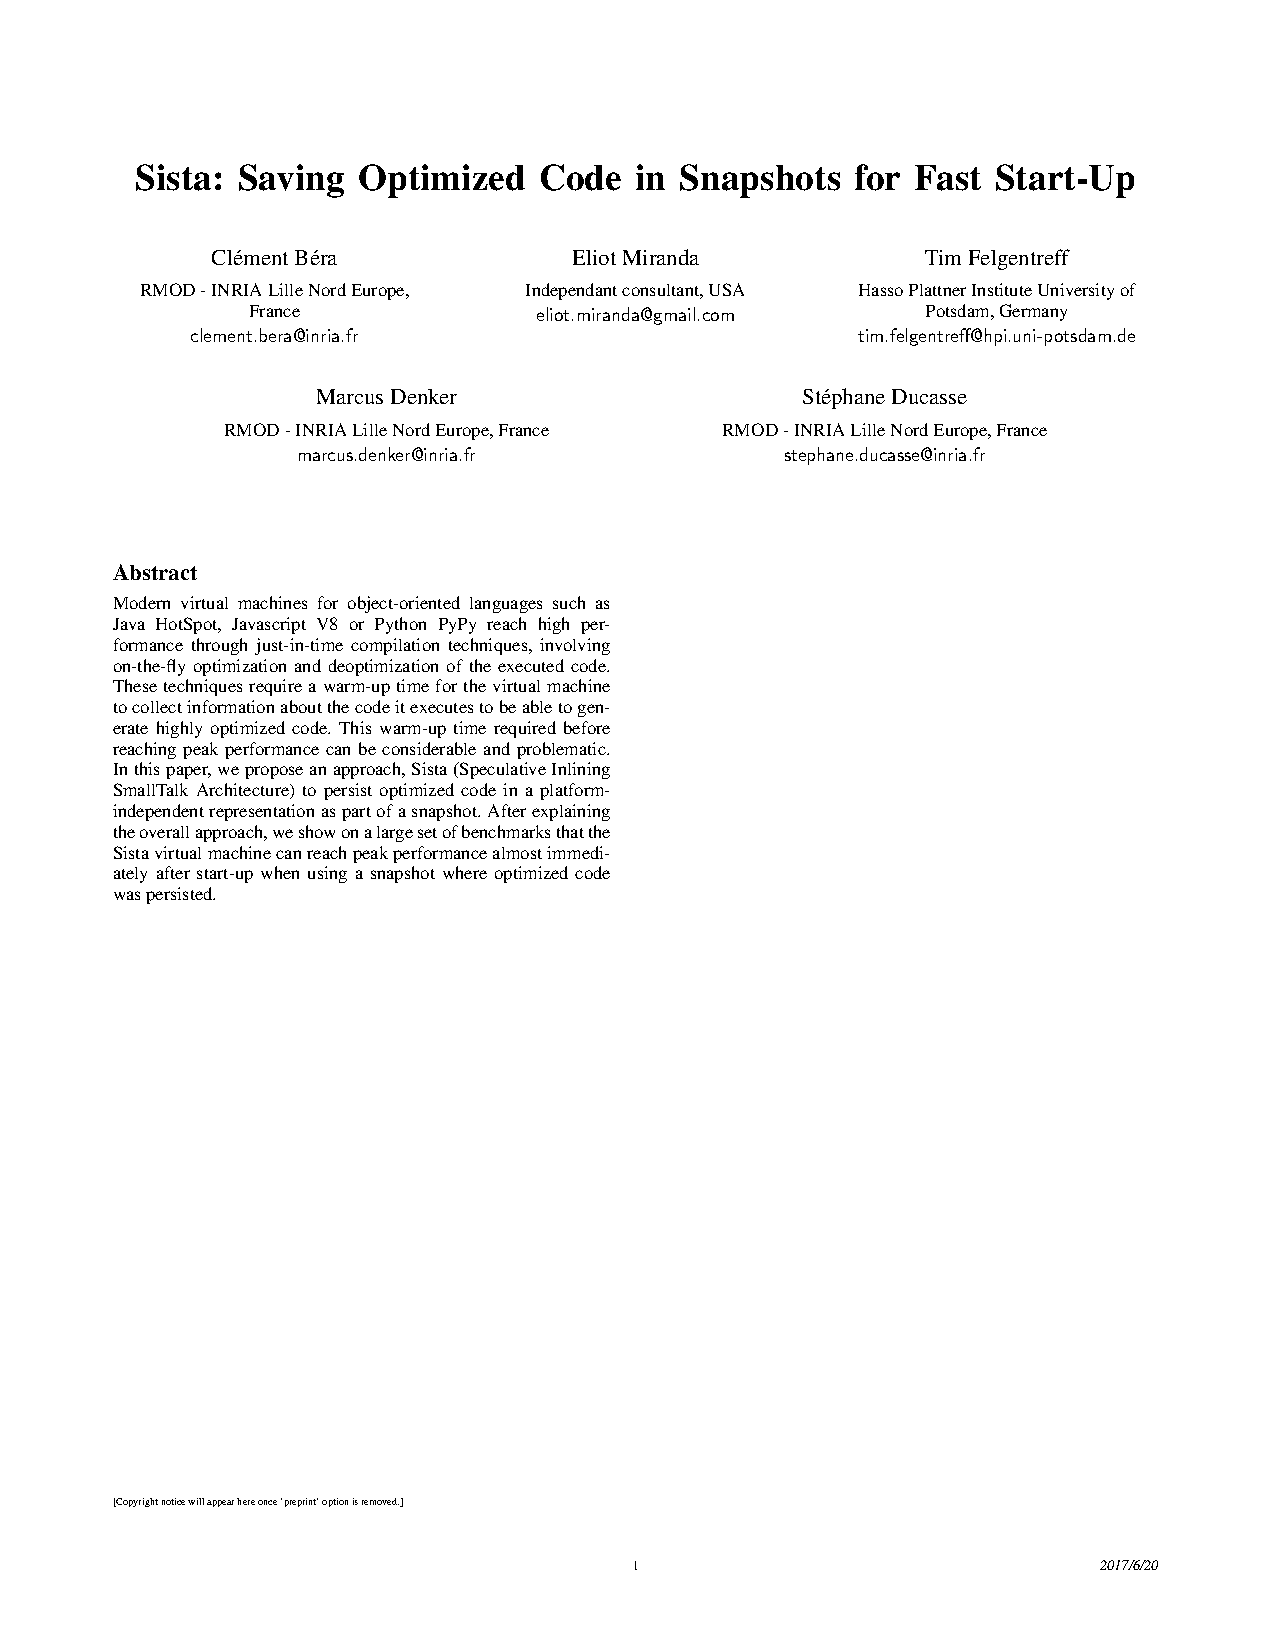
\includegraphics[width=\linewidth]{Bench}
        \caption{Benchmark measurements}
        \label{fig:measure}
    \end{center}
\end{figure}

\subparagraph{A*.}

The A* benchmark is a good approximation for applications where many objects collaborate. It measures parsing of large strings that define the layout of the nodes, message sending between each node, arithmetic to calculate costs, and collection operations. In the benchmark, we alternately parse and traverse two different graphs with 2,500 and 10,000 nodes, respectively. It is also a good benchmark for inlining block closures that are used in iterations.

Figure~\ref{fig:measure}(a) shows that adding counters to the VM comes with a slight overhead. A cold start for the benchmarks manages to improve the performance, but due to the ongoing optimisations in the beginning of the measurments, the error is extremely large and thus the run is not significantly faster. Measuring the warmed up image, we see a significant improvement being about 30\% faster.                          

\subparagraph{Binary tree.}

The binary tree benchmark allocates, walks and deallocates binary trees. The benchmark is parameterized with  the maximum tree depth, which we have set to 10.

In this benchmark, peak performance of Sista is about 25\% faster than the standard VM, with very little error (Figure~\ref{fig:measure}(b)). The overhead of optimisation during a cold start leaves it around 5\% behind warm start.

\subparagraph{JSON parsing.}

We test a JSON parser written in Smalltalk as it parses a constant, minified, well-formed JSON string of 25 Kilobytes. This benchmark is heavy on nested loops and string operations, as well as a lot of parsing rules that call each other.

We can see a peak-performance is about 20\% faster (Figure~\ref{fig:measure}(c)). Even from a cold start Sista quickly improves performance to about 10\% faster than Cog.

\subparagraph{Richards.}

Richards is an OS kernel simulation benchmark that focuses on message sending between objects and block invocation. We ran this benchmark with the customary idle task, two devices, two handler tasks, and a worker, and filled the work queue of the latter three.

Figure \ref{fig:measure}(d) again shows a clear decrease in performance after adding counters to the VM. For this benchmark, warm-up is very quick even with our additional optimisations. The top-level benchmarking method is optimised very quickly, and only six optimised methods are installed in total. This quick warm-up means there is no significant difference between the cold start Sista and the warmed up image. Both cases are a little over 10\% faster than the Cog VM without counters.

\subparagraph{k-Nucleotide.}

This benchmark reads a 2.4 MB DNA sequence string and counts all occurrences of nucleotides of lengths 1 and 2, as well as a number of specific sequences. It is a benchmark meant to test the performance of dictionaries in different languages, but serves well to test our inlining of small methods into loops.

The benchmark runs much slower than the others due to the large input, taking over 4 minutes to complete. Sista manages to optimise it to be about 10\% faster, with the cold start showing that the optimisation takes a while to amortize (Figure~\ref{fig:measure}(e)).

\subparagraph{Thread ring benchmark.}

The Thread ring benchmark switches from thread to thread (green threads) passing one token between threads. Each iteration, 503 green threads are created and the token is passed around 5,000,000 times.

From an unoptimised snapshot, the first iteration of this benchmark is bound to be slow with our architecture, because multiple threads exist with the same code on the stack, each asking the profiler to optimise the same methods, while the optimiser refuses to do so because an optimised function already exists for the frequently used code. This might be a reason for the large error (Figure~\ref{fig:measure}(f)). Started again after warm-up, the optimised code runs over 40\% faster than the standard VM.

\subparagraph{Blowfish.}

Blowfish tests the performance of bit operations by encrypting and decrypting messages. Each iteration encrypts and decrypts 20 messages with 20 different keys.

Figure~\ref{fig:measure}(g) shows no significant differences between Cog, Cog with counters and Sista after warm-up. We explain this with the fact that most time here is spent in bit operations and very little message sending takes place in comparison. The inlining does not significantly improve the performance in this case, and bit shift, logical AND and OR operations are already treated specially in the default bytecode set so there is not much performance to gain.

\subparagraph{DeltaBlue.}

DeltaBlue is a constraint solver, it tests polymorphic message sending and graph traversal. Each iteration tests updating a chain of 5000 connected variables once with equality constraints and once with a simple arithmetic scale constraint.

For our default parameters, the benchmark shows no significant differences between Cog, Cog with counters and Sista -- all errors overlap (\ref{fig:measure}(h)). We have found that increasing the maximum allowed inlining depth to 14 levels (rather than 12, as used for the other benchmarks), allows the optimiser to produce code that is 20\% faster, but it has caused performance problems other benchmarks, so we chosen not to change the variable for the time being.

\subparagraph{Comments.}

We ran our VM profiler to profile the VM C code, but as for real world application, the time spent in the baseline JIT compiler generating machine code from bytecode is less than 1\% of the total execution time. As the runtime switches from interpreted code to machine code at second invocation for most functions and at first invocation for optimised functions, the time lost here is too small to be shown on our graphics. In fact, the time lost here is not significant compared to the variation so it is difficult to evaluate in our current setting. We believe that using a back-end doing many more machine low-level optimisations would increase the machine code compilation time and in this case we would be able to see a difference between the first run of pre-heated snapshot and second run as the VM still needs to produce the machine code for the optimised bytecoded functions.

\begin{figure}[h!]
    \begin{center}
        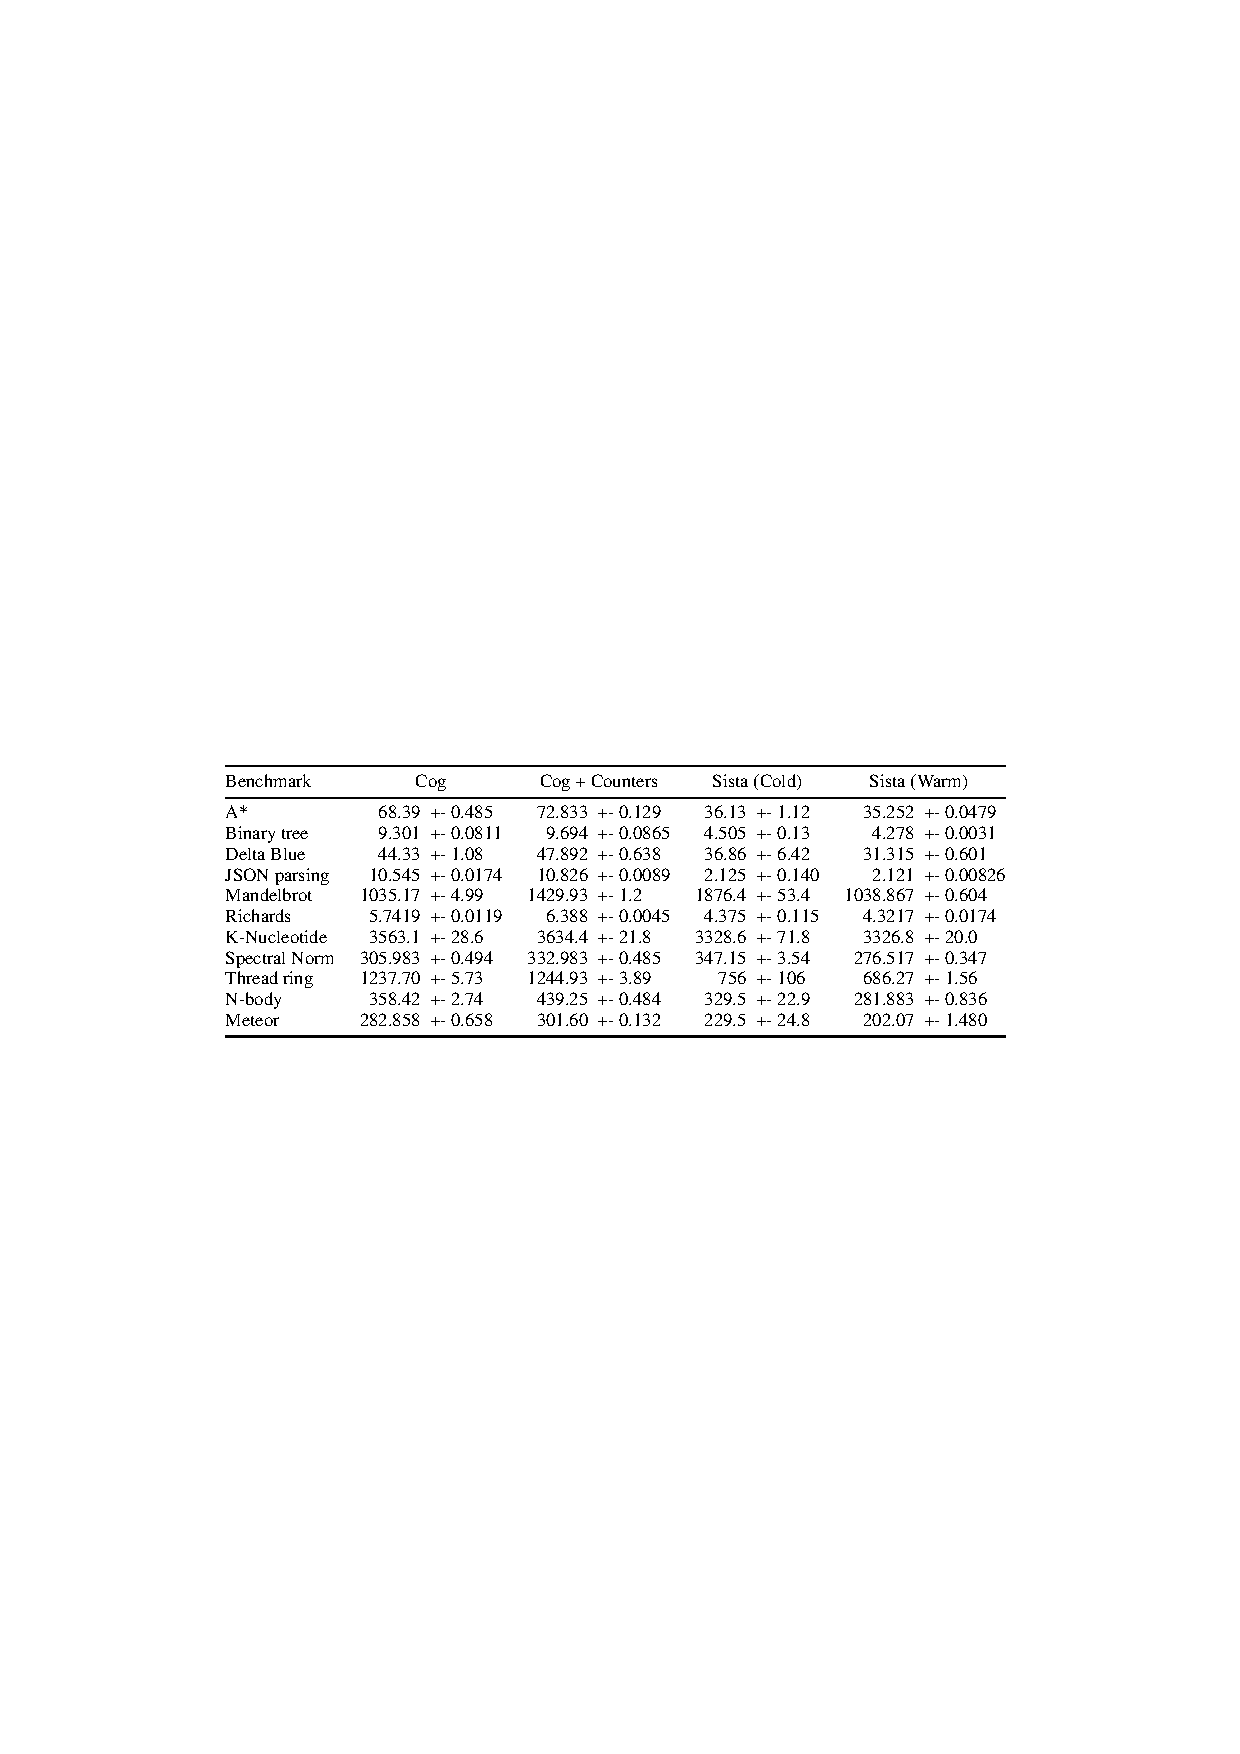
\includegraphics[width=\linewidth]{BenchTable}
        \caption{Benchmark results (standard errors in avg ms, 90\% confidence interval)}
        \label{tbl:benchmark}
    \end{center}
\end{figure}

Our optimiser is controlled by a number of variables that have been heuristically chosen to give good performance in a variety of cases. These include, among others, global settings for inlining depth, the allowed maximum size of optimised methods as well as methods to be inlined, as well as the time allowed for the optimiser to create an optimised method before it is aborted. We have found that for certain benchmarks (such as DeltaBlue), these variables can have a great impact. We are working on fine-tuning these default values, as well as enabling heuristics to dynamically adapt these values depending on the application.

\section{Other validations}
\label{sec:otherValid}

To evaluate our infrastructure, we tried two other innovative techniques in addition to measuring benchmarks. On the one hand, we built an experimental technique to validate runtime deoptimisation using partial evaluation. On the other hand, we built a type inferencer using the runtime information extracted from inline caches. The promising results of the type inferencer confirm that the runtime information is quite precise and should give Scorch valuable hints to direct compiler optimisations.

\subsection{Experimental validation of the deoptimiser}

The speculative optimisations in the Sista VM enable many performance optimisations. However, they also introduce significant complexity. The compiler optimisations themselves, as well as the deoptimisation mechanism are complex and error prone. To stabilize Scorch, we designed a new approach to validate the correctness of dynamic deoptimisation. The approach~\cite{Bera16a} consists of the symbolic execution of an optimised and a non optimised v-function side by side, deoptimising the abstract stack at each point where dynamic deoptimisation is possible and comparing the deoptimised and non optimised abstract stack to detect bugs. 

Although this approach is interesting, the complexity required to maintain a good symbolic executor is significant compared to the time available for the maintenance of the overall VM. In other VMs such as V8~\cite{V8}, dynamic deoptimisation is stabilised using a "deopt-every-n-time" approach: the program run is forced to deoptimise the stack regularly (every n deoptimisation point met). This approach is way simpler to maintain and finds in practice a similar number of bugs than the approach built. We are now using a "deopt-every-n-time" approach to validate the deoptimisation of functions.

\subsection{Assessment of the runtime information quality}

Thanks to a new primitive method, any Pharo program, including Scorch, may request Cogit to provide the runtime information of a specific function. This runtime information is composed of the types met and functions called at each virtual call and the profiling counter values. To assess the quality of the runtime information provided for each virtual call, we built an approach called \emph{inline-cache type inference} (ICTI) to augment the precision of fast and simple type inference algorithms~\cite{Milo16a}. 

ICTI uses type information available in the inline caches during multiple software runs, to provide a ranked-list of possible classes that most likely represent a variable's type. We evaluated ICTI through a proof-of-concept that we implemented in Pharo Smalltalk. Analyzing the top-$n$+2 inferred types (where $n$ is the number of recorded runtime types for a variable) for 5486 variables from four different software systems (Glamour~\cite{Bung09a}, Roassal2~\cite{Pena13a}, Morphic~\cite{Fern07y} and Moose~\cite{Girb10a, Duca05a, Duca00b}) show that ICTI produces promising results for about 75\% of the variables. For more than 90\% of variables, the correct runtime type was present among first ten inferred types. Our ordering shows a twofold improvement when compared with the unordered base approach, \ie for a significant number of variables for which the base approach offered ambiguous results, ICTI was able to promote the correct type to the top of the list.

Based on this results, we believe the runtime information extracted from the first runs to be quite reliable. In any case, this information is used only to direct compiler optimisation: if the runtime information is not correct, the code is executed slower but correctly.

%%%%%%%%%%%%%%%%%%%%%%%%%%%%%%%%%%%%%%%%%%%%%%%%%%%%%%%%%%%%%%%%%%%%%%%%%%%%%%%%%%%%%%%%%%%%%%%%%%%%%%%%%%%%%%%%%%%%%%%%%%%%%%%%%%%%%%%%%%%%%%%%%%%

\section*{Conclusion}

This chapter validates Sista by showing on a range of benchmarks the performance gain of the architecture. The next Chapter discusses the future works that could be considered based on this thesis.

\ifx\wholebook\relax\else
    \end{document}
\fi
\ifx\wholebook\relax\else

% --------------------------------------------
% Lulu:

    \documentclass[a4paper,12pt,twoside]{../includes/ThesisStyle}

	\usepackage[T1]{fontenc} %%%key to get copy and paste for the code!
%\usepackage[utf8]{inputenc} %%% to support copy and paste with accents for frnehc stuff
\usepackage{times}
\usepackage{ifthen}
\usepackage{xspace}
\usepackage{alltt}
\usepackage{latexsym}
\usepackage{url}            
\usepackage{amssymb}
\usepackage{amsfonts}
\usepackage{amsmath}
\usepackage{stmaryrd}
\usepackage{enumerate}
\usepackage{cite}
%\usepackage[pdftex,colorlinks=true,pdfstartview=FitV,linkcolor=blue,citecolor=blue,urlcolor=blue]{hyperref}
\usepackage{xspace}
%\usepackage{graphicx}
\usepackage{subfigure}
\usepackage[scaled=0.85]{helvet}
        
        
\newcommand{\sepe}{\mbox{>>}}
\newcommand{\pack}[1]{\emph{#1}}
\newcommand{\ozo}{\textsc{oZone}\xspace}
\newcommand\currentissues{\par\smallskip\textbf{Current Issues -- }}

\newboolean{showcomments}
\setboolean{showcomments}{true}
\ifthenelse{\boolean{showcomments}}
  {\newcommand{\bnote}[2]{
	\fbox{\bfseries\sffamily\scriptsize#1}
    {\sf\small$\blacktriangleright$\textit{#2}$\blacktriangleleft$}
    % \marginpar{\fbox{\bfseries\sffamily#1}}
   }
   \newcommand{\cvsversion}{\emph{\scriptsize$-$Id: macros.tex,v 1.1.1.1 2007/02/28 13:43:36 bergel Exp $-$}}
  }
  {\newcommand{\bnote}[2]{}
   \newcommand{\cvsversion}{}
  } 


\newcommand{\here}{\bnote{***}{CONTINUE HERE}}
\newcommand{\nb}[1]{\bnote{NB}{#1}}
\newcommand{\fix}[1]{\bnote{FIX}{#1}}
%%%% add your own macros 

\newcommand{\sd}[1]{\bnote{Stef}{#1}}
\newcommand{\ja}[1]{\bnote{Jannik}{#1}}
\newcommand{\na}[1]{\bnote{Nico}{#1}}
%%% 


\newcommand{\figref}[1]{Figure~\ref{fig:#1}}
\newcommand{\figlabel}[1]{\label{fig:#1}}
\newcommand{\tabref}[1]{Table~\ref{tab:#1}}
\newcommand{\layout}[1]{#1}
\newcommand{\commented}[1]{}
\newcommand{\secref}[1]{Section \ref{sec:#1}}
\newcommand{\seclabel}[1]{\label{sec:#1}}

%\newcommand{\ct}[1]{\textsf{#1}}
\newcommand{\stCode}[1]{\textsf{#1}}
\newcommand{\stMethod}[1]{\textsf{#1}}
\newcommand{\sep}{\texttt{>>}\xspace}
\newcommand{\stAssoc}{\texttt{->}\xspace}

\newcommand{\stBar}{$\mid$}
\newcommand{\stSelector}{$\gg$}
\newcommand{\ret}{\^{}}
\newcommand{\msup}{$>$}
%\newcommand{\ret}{$\uparrow$\xspace}

\newcommand{\myparagraph}[1]{\noindent\textbf{#1.}}
\newcommand{\eg}{\emph{e.g.,}\xspace}
\newcommand{\ie}{\emph{i.e.,}\xspace}
\newcommand{\ct}[1]{{\textsf{#1}}\xspace}


\newenvironment{code}
    {\begin{alltt}\sffamily}
    {\end{alltt}\normalsize}

\newcommand{\defaultScale}{0.55}
\newcommand{\pic}[3]{
   \begin{figure}[h]
   \begin{center}
   \includegraphics[scale=\defaultScale]{#1}
   \caption{#2}
   \label{#3}
   \end{center}
   \end{figure}
}

\newcommand{\twocolumnpic}[3]{
   \begin{figure*}[!ht]
   \begin{center}
   \includegraphics[scale=\defaultScale]{#1}
   \caption{#2}
   \label{#3}
   \end{center}
   \end{figure*}}

\newcommand{\infe}{$<$}
\newcommand{\supe}{$\rightarrow$\xspace}
\newcommand{\di}{$\gg$\xspace}
\newcommand{\adhoc}{\textit{ad-hoc}\xspace}

\usepackage{url}            
\makeatletter
\def\url@leostyle{%
  \@ifundefined{selectfont}{\def\UrlFont{\sf}}{\def\UrlFont{\small\sffamily}}}
\makeatother
% Now actually use the newly defined style.
\urlstyle{leo}



	\usepackage{amsmath,amssymb}             % AMS Math
% \usepackage[french]{babel}
\usepackage[latin1]{inputenc}
\usepackage[T1]{fontenc}
\usepackage[left=1.5in,right=1.3in,top=1.1in,bottom=1.1in,includefoot,includehead,headheight=13.6pt]{geometry}
\renewcommand{\baselinestretch}{1.05}

\usepackage{multicol}

% Table of contents for each chapter

\usepackage[nottoc, notlof, notlot]{tocbibind}
\usepackage{minitoc}
\setcounter{minitocdepth}{1}
\mtcindent=15pt
% Use \minitoc where to put a table of contents

\usepackage{enumitem}

\usepackage{aecompl}

% Glossary / list of abbreviations

%\usepackage[intoc]{nomencl}
%\renewcommand{\nomname}{List of Abbreviations}
%
%\makenomenclature

% My pdf code

\usepackage[pdftex]{graphicx}
\usepackage[a4paper,pagebackref,hyperindex=true]{hyperref}

\usepackage{pgfplotstable,booktabs,colortbl}
\pgfplotsset{compat=1.8}

% Links in pdf
\usepackage{color}
\definecolor{linkcol}{rgb}{0,0,0.4} 
\definecolor{citecol}{rgb}{0.5,0,0} 

% Change this to change the informations included in the pdf file

% See hyperref documentation for information on those parameters

\hypersetup
{
bookmarksopen=true,
pdftitle="Sista: a Metacircular Architecture for Runtime Optimisation Persistence",
pdfauthor="Clement BERA", 
pdfsubject="Thesis", %subject of the document
%pdftoolbar=false, % toolbar hidden
pdfmenubar=true, %menubar shown
pdfhighlight=/O, %effect of clicking on a link
colorlinks=true, %couleurs sur les liens hypertextes
pdfpagemode=None, %aucun mode de page
pdfpagelayout=SinglePage, %ouverture en simple page
pdffitwindow=true, %pages ouvertes entierement dans toute la fenetre
linkcolor=linkcol, %couleur des liens hypertextes internes
citecolor=citecol, %couleur des liens pour les citations
urlcolor=linkcol %couleur des liens pour les url
}

% definitions.
% -------------------

\setcounter{secnumdepth}{3}
\setcounter{tocdepth}{1}

% Some useful commands and shortcut for maths:  partial derivative and stuff

\newcommand{\pd}[2]{\frac{\partial #1}{\partial #2}}
\def\abs{\operatorname{abs}}
\def\argmax{\operatornamewithlimits{arg\,max}}
\def\argmin{\operatornamewithlimits{arg\,min}}
\def\diag{\operatorname{Diag}}
\newcommand{\eqRef}[1]{(\ref{#1})}

\usepackage{rotating}                    % Sideways of figures & tables
%\usepackage{bibunits}
%\usepackage[sectionbib]{chapterbib}          % Cross-reference package (Natural BiB)
%\usepackage{natbib}                  % Put References at the end of each chapter
                                         % Do not put 'sectionbib' option here.
                                         % Sectionbib option in 'natbib' will do.
\usepackage{fancyhdr}                    % Fancy Header and Footer

% \usepackage{txfonts}                     % Public Times New Roman text & math font
  
%%% Fancy Header %%%%%%%%%%%%%%%%%%%%%%%%%%%%%%%%%%%%%%%%%%%%%%%%%%%%%%%%%%%%%%%%%%
% Fancy Header Style Options

\pagestyle{fancy}                       % Sets fancy header and footer
\fancyfoot{}                            % Delete current footer settings

%\renewcommand{\chaptermark}[1]{         % Lower Case Chapter marker style
%  \markboth{\chaptername\ \thechapter.\ #1}}{}} %

%\renewcommand{\sectionmark}[1]{         % Lower case Section marker style
%  \markright{\thesection.\ #1}}         %

\fancyhead[LE,RO]{\bfseries\thepage}    % Page number (boldface) in left on even
% pages and right on odd pages
\fancyhead[RE]{\bfseries\nouppercase{\leftmark}}      % Chapter in the right on even pages
\fancyhead[LO]{\bfseries\nouppercase{\rightmark}}     % Section in the left on odd pages

\let\headruleORIG\headrule
\renewcommand{\headrule}{\color{black} \headruleORIG}
\renewcommand{\headrulewidth}{1.0pt}
\usepackage{colortbl}
\arrayrulecolor{black}

\fancypagestyle{plain}{
  \fancyhead{}
  \fancyfoot{}
  \renewcommand{\headrulewidth}{0pt}
}

\usepackage{algorithm}
\usepackage[noend]{algorithmic}

%%% Clear Header %%%%%%%%%%%%%%%%%%%%%%%%%%%%%%%%%%%%%%%%%%%%%%%%%%%%%%%%%%%%%%%%%%
% Clear Header Style on the Last Empty Odd pages
\makeatletter

\def\cleardoublepage{\clearpage\if@twoside \ifodd\c@page\else%
  \hbox{}%
  \thispagestyle{empty}%              % Empty header styles
  \newpage%
  \if@twocolumn\hbox{}\newpage\fi\fi\fi}

\makeatother
 
%%%%%%%%%%%%%%%%%%%%%%%%%%%%%%%%%%%%%%%%%%%%%%%%%%%%%%%%%%%%%%%%%%%%%%%%%%%%%%% 
% Prints your review date and 'Draft Version' (From Josullvn, CS, CMU)
\newcommand{\reviewtimetoday}[2]{\special{!userdict begin
    /bop-hook{gsave 20 710 translate 45 rotate 0.8 setgray
      /Times-Roman findfont 12 scalefont setfont 0 0   moveto (#1) show
      0 -12 moveto (#2) show grestore}def end}}
% You can turn on or off this option.
% \reviewtimetoday{\today}{Draft Version}
%%%%%%%%%%%%%%%%%%%%%%%%%%%%%%%%%%%%%%%%%%%%%%%%%%%%%%%%%%%%%%%%%%%%%%%%%%%%%%% 

\newenvironment{maxime}[1]
{
\vspace*{0cm}
\hfill
\begin{minipage}{0.5\textwidth}%
%\rule[0.5ex]{\textwidth}{0.1mm}\\%
\hrulefill $\:$ {\bf #1}\\
%\vspace*{-0.25cm}
\it 
}%
{%

\hrulefill
\vspace*{0.5cm}%
\end{minipage}
}

\let\minitocORIG\minitoc
\renewcommand{\minitoc}{\minitocORIG \vspace{1.5em}}

\usepackage{multirow}
\usepackage{slashbox}

\newenvironment{bulletList}%
{ \begin{list}%
	{$\bullet$}%
	{\setlength{\labelwidth}{25pt}%
	 \setlength{\leftmargin}{30pt}%
	 \setlength{\itemsep}{\parsep}}}%
{ \end{list} }

\newtheorem{definition}{D�finition}
\renewcommand{\epsilon}{\varepsilon}

% centered page environment

\newenvironment{vcenterpage}
{\newpage\vspace*{\fill}\thispagestyle{empty}\renewcommand{\headrulewidth}{0pt}}
{\vspace*{\fill}}



	\graphicspath{{.}{../figures/}}
	\begin{document}
\fi

\chapter{Future work}
\label{chap:futureWork}
\minitoc

This chapter discusses future work related to Sista. The focus is on research-oriented future work, but the first two sections also mention engineering-oriented future work (for instance, moving the architecture to production).

Section \ref{sec:archEvo} describes the evolution planned or considered for the overall architecture. Section \ref{sec:newOpt} discusses specifically the optimisations that could be implemented in Scorch and Cogit. Section \ref{sec:useCase} details how the application of Sista on a real-world application requiring quick start-ups would be very valuable to validate further the architecture. Lastly, Section \ref{sec:energy} discusses briefly the potentially low energy consumption of the Sista VM and how it could be valuable in specific use-cases.

\section{Architecture evolution}
\label{sec:archEvo}

This section details the evolution of the Sista architecture that are worth investigating. Section \ref{ss:FWInterface} describes the potential evolution of the interface VM-language: Sista is currently using an extended bytecode set to communicate between Scorch and Cogit, another representation may be better. Section \ref{ss:FWIDE} explains the on-going work to integrate Sista with the development tools. The evaluation of the memory footprint used by the Sista runtime is precised in Section \ref{ss:FWMemFootprint}. Section \ref{ss:FWPlatDep} discusses the current platform-dependencies of the persistence of the runtime state across start-ups and how these dependencies could be avoided. Section \ref{ss:FWProduct} briefly states the on-going work to move Sista to production.

\subsection{Interface VM-language}
\label{ss:FWInterface}

\paragraph{Stack-based or register-based IR.}The v-functions discussed in the thesis are currently encoded in a stack-based bytecode Intermediate Representation (IR). Stack-based IRs are usually considered as difficult to deal with in optimising compilers, so this can be seen as a problem. For this reason, Scorch decompiles the v-function to a register-based IR (similar to TAC\footnote{Three Address Code.}, but some operations such as virtual calls may have more than three parameters), performs the optimisations and translates it back to the stack-based bytecode. Cogit then takes the stack-based bytecode as input, and translates it to a register-based IR to generate the n-function. 

The stack-based extended bytecode sets has two main issues:
\begin{itemize}
	\item \textbf{Loss of information:} Scorch IR has significant information about the instructions (liveness, uses) than the stack-based bytecode. This information is lost during the translation to the stack-based bytecode, while it may be valuable for Cogit to perform efficiently low-level optimisations.
	\item \textbf{redundant conversion:} When compiling using Sista's optimising JIT, unoptimised v-functions are compiled by Scorch to optimised v-functions and then by Cogit to optimised n-functions. It feels a bit redundant to take a stack-based IR (bytecode of the v-function), translate it to a register-based IR (Scorch IR), then translate it back to a stack-based IR (extended bytecode of the optimised v-function) and lastly translate it to a register-based IR (Cogit's IR), as shown in the left part of Figure \ref{fig:FutureWorkredundant}. One could consider encoding optimised v-functions in a register-based IR, to avoid two translations.
\end{itemize}

\begin{figure}[h!]
    \begin{center}
        \includegraphics[width=0.7\linewidth]{FutureWorkredondant}
        \caption{redundant conversion}
        \label{fig:FutureWorkredundant}
    \end{center}
\end{figure}

However, the extended bytecode set was designed stack-based for two relevant reasons:
\begin{itemize}
	\item \textbf{Compatibility:} The existing bytecode set is stack-based, and having the extended bytecode set stack-based allows us to generate optimised functions using existing instructions and not only new ones. This was very convenient to have quickly a working version of Sista (only the new unsafe operations used needed to work to have the architecture working).
	\item \textbf{Machine-independent:} A stack-based representation allows one to abstract away from low-level details such as the exact number of registers. To abstract away from the exact number of registers, both a stack-based IR and a register-based IR with an infinite number of registers are possible. 
	Although at first look it seems the register-based solution is easier to deal with, experts such as the ones which designed WebAssembly~\cite{WebAssembly} chose to use a stack-based IR over a register-based IR. It is not clear which solution is better.
\end{itemize}	 

One future work is to design another extended bytecode set, register-based, and to evaluate the complexity of the representation in the back-end of Scorch and the front-end of Cogit, as shown on the right part of Figure \ref{fig:FutureWorkredundant}.

\paragraph{Lower-level representation.}The optimised v-functions are encoded in a quite high-level representation. For example, instructions like array accesses generate multiple native instructions. The extended bytecode set is quite high-level because it abstracts away from:
\begin{itemize}
	\item the memory representation of objects.
	\item the processor used.
\end{itemize}

We believe abstracting away from the processor used was a good idea as it allows one to use snapshot to persist the optimised state across multiple start-ups. However, snapshots are already dependent on the memory representation of objects used, so one could implement a new representation of optimised v-functions with a lower-level representation, object representation dependent but still processor independent. This would allow Scorch to perform additional optimisations, such as better constant propagation (Some constants are currently hidden in high-level instructions), which are currently hard to support in Cogit.

Currently, only the VM code is aware of the memory representation of object. Hence, using such a lower-level representation would require to duplicate the knowledge about the memory representation of objects from the VM code-base to Pharo, so Scorch could be aware of it. 

\subparagraph{Summary.}To summarize, one could change Sista so optimised v-functions would be encoded in a lower-level representation instead of the extended bytecode set. Such changes would make Scorch dependent of the memory representation of objects, while keeping it independent from the processor used. Some code would need to be duplicated from the VM code-base to Pharo to make Scorch aware of the internal memory representation of objects. Scorch would be able to produce more optimised code, performing optimisations that are currently difficult to implement in Cogit, yielding hopefully better performance.

\subparagraph{Implementation.}To implement such a solution, one could build a back-end for Scorch targeting the abstract assembly instructions set featured by the Cog VM, called Lowcode~\cite{Salg16a}, similar to WebAssembly~\cite{WebAssembly}. Lowcode features low-level instructions, compiled almost in most processors one-to-one to machine instructions. The future work is to implement such a back-end for Scorch and evaluate the complexity and the performance.

\subsection{Development tools integration}
\label{ss:FWIDE}

In Sista, Scorch is an unoptimised v-functions to optimised v-functions compiler, running in the same runtime as the application. Although this design has several advantages, there is a major draw-back: when the programmer accesses the reification of a stack frame, depending on the optimisation state, an optimised frame might be shown. 

In some cases, for example when the programmer is working on Scorch itself, it is relevant to show in the development tools the optimised frames. In other cases, for example when the programmer is working in an end-user application on top of Pharo, development tools should show only unoptimised frames by transparently deoptimising stack frames.

We are now adapting the debugging tools to request deoptimise stack frames when needed. To do so, we are adding a development tool setting: one may or may not want to see the stack internals, depending on what one wants to implement.

\subsection{Memory footprint evaluation}
\label{ss:FWMemFootprint}

When implementing an optimising JIT, it is relevant to evaluate the memory footprint of the optimised code and the deoptimisation metadata. In our context, such an evaluation would be very interesting as:
\begin{itemize}
	\item \textbf{Split architecture:} Due to the split between Scorch and Cogit, optimised functions are present both as v-functions and n-functions, and each of them has different deoptimisation metadata, potentially increasing the memory footprint. 
	\item \textbf{Persistence:} As optimised v-functions are persisted across start-ups, it is interesting to know the size of the optimised v-functions and the corresponding deoptimisation metadata that is persisted.
\end{itemize}

Two future works are planned in this direction:
\begin{itemize}
	\item Does the split in the optimising JIT induce memory overhead compared to a classical function-based optimising JIT, and how big is the overhead?
	\item What is the size of the optimised v-functions and the corresponding deoptimisation metadata that is persisted across start-up?
\end{itemize}

We did not evaluate the memory footprint because currently the deoptimisation metadata of Scorch is kept uncompressed. As Scorch deoptimiser requires to read deoptimisation metadata, compressing the metadata requires to write a decompressor which is, as all the deoptimiser code, independent from the rest of the system. This is possible but requires a certain amount of engineering work, which is the reason why we postponed it.

\subsection{Platform-dependency}
\label{ss:FWPlatDep}

In Pharo, snapshots are independent of the processor and the OS used. It is proven as the same snapshot can be deployed on x86, ARMv6 and MIPSEL, as well as on Windows, Mac OS X, iOS, Linux, Android or RISC OS. However, the snapshots are dependent on the machine word size: 32 bit or 64 bit snapshots are not compatible. They are not compatible because the size of managed pointers is different, but also because the representation of specific objects, such as floating numbers, is different. It is however possible to convert offline a 32 bit snapshot to 64 bit and vice-versa. 

As some optimisations related to number arithmetics, such as overflow checks elimination, depends on the number representations, Scorch is currently dependent on the machine word size. A fully portable solution would either need not to do optimisations on machine word specific number representations or deoptimise the affected code on start-up.

\subsection{Productisation}
\label{ss:FWProduct}

With the current version, the Sista VM is able to run all our benchmark suite. We are now able to do part of our development with the development tools, written in Pharo, running on the Sista VM. We still have work to do in the integration with the development tools, especially the debugger, but it seems that the biggest part of the work has been done. 

There are still some edge cases where the Sista VM is unstable, which still need to be fixed, but most code can be run on top of the Sista VM as it would be run on the production VM. We have started to integrate the dependencies of Sista in Pharo, such as the new implementation of closures, the new bytecode set or read-only objects. We are now looking forward to integrate Scorch in Pharo.

\section{New optimisations}
\label{sec:newOpt}

Another direction for future work is the implementation of new optimisations in Scorch or Cogit. 

\subsection{State-of-the-art optimisations}

To compare Sista against other optimising JITs efficiently, the next thing to do is to implement all the state-of-the-art compiler optimisation in Scorch and Cogit. Scorch lacks multiple common optimisation passes, including important ones for performance such as floating-pointer related optimisations or advanced escape analysis. Cogit features a naive register allocator to set registers in its dynamic templates, but we have plan to build a more advanced one and evaluate the performance difference. 

\subsection{New optimisations}

Aside from existing optimisations, one could implement new optimisations that are not present in other compilers. 

One way to do so is to have new ideas on how to optimise code, to design and implement new algorithms. This is far from trivial as many experts have worked in compiler optimisations in other compilers, but, it is theoretically possible.

Alternatively, one could describe how traditional optimisations are implemented in the context of the split architecture present in Sista. For example, one could explain which optimisation should be implemented in Scorch, which one should be implemented in Cogit, which one should be implemented partly with both and which annotations are required in the optimised v-functions to communicate extra information from Scorch to Cogit. 

Lastly, and most interestingly, one could work on Smalltalk-specific optimisations that are not possible or not relevant in other programming languages because they do not usually support the unconventional features present in Smalltalk.

Indeed, Smalltalk provides some unconventional operations that are not usually available in other object-oriented languages. These operations are problematic for the optimising JIT. The main operations we are talking about are become, described in Section \label{par:become} and heavy stack manipulation APIs on reified stack frames detailed in Section \ref{par:frameToContext}. 

In each case, the feature has implications in the context of an optimising JIT as at any interrupt point, there any temporary variable of the optimised stack frame, or worst, any internal state (sender frame, program counter, etc.) could be edited to any object in the heap. This would invalidate all assumptions taken at compilation time by Scorch.

Fortunately, all these operations are uncommon in a normal Smalltalk program at runtime. They are usually used for implementing the debugging functionalities of Pharo. Currently, profiling production applications does not show we could earn noticeable performance if we would optimise such cases. The current solution is therefore to always deoptimise the stack frames involved when such unconventional operations happen. In the case of become, if a temporary variable in a stack frame executing an optimised method is edited, the frame is deoptimised. In the case of the stack manipulation, if the reification of the stack is mutated from the language, we deoptimise the corresponding mutated stack frames.

However, in specific libraries or workflow, such operations may be common enough to have some impact on performance. Especially, continuations and exceptions are built in Pharo in the language on top of the stack manipulation features, and a few libraries use them extensively. It could be possible to have Scorch aware of these features and to handle them specifically. Scorch would for example mark some temporary variables as being accessed frequently from the outside of the function: such temporaries would not be optimised and the deoptimisation metadata would include information on how to access those temporaries of inlined functions directly in the optimised frame. Optimising such features would allow to have efficient continuations and exceptions, in a similar way to the optimisation of exceptions described in \cite{Ogas01a}. 

\section{Application of Sista for quick start-ups}
\label{sec:useCase}

One point that is a bit unclear is how to use the Sista for quick start-up in a real-world application. It is possible to persist optimised functions across start-ups. However, how are the optimised functions generated in the first place? Are they generated from warm-up runs using a test suite or are they generated the first day the application is running?

A good example on how to use persisted optimisations across start-up is the success story of Azul~\cite{Azul}: a trading bank claims that they are able to use the optimised functions generated the day N-1 to improve the start-up performance of the day N. Another good example is the user-base of the cloneable Java VM~\cite{Kawa07a}.

It seems that depending on the use-case where start-up performance matters (distributed application with short-lived slaves, such as the ones on Amazon lambda, Android application or Web pages), different frameworks and solutions require to be set up to improve start-up performance using persisted optimisations. 

It would be very valuable to focus on one of those use-cases and build a solid framework showing how to use the persistence of optimisations to reduce warm-up time and evaluate what is the cost for the application programmer. Does the programmer have to do something specific to persist the optimisations as part of the deployment (warm-up runs, etc.) or is it done automatically as part of a framework?

In the case of distributed application on Amazon lambda, slaves may live down to a couple seconds in case of a high-variant demand, so that there are very few slaves rent when the application is unused and a lot of slaves when the application is heavily used. Is it possible to build a framework that automatically learn from the life of previous slaves what optimised functions are worth keeping, so when a new short-lived slaved is instantiated, it can reach peak performance very quickly?

In the case of web pages, is it possible to build a global cache so all frequently used web pages would have pre-optimised code available from the runs of the previous users? How would such a design work with modern security requirements?

All these applications of the persistence of optimisations across start-ups of Sista are very interesting and could be analysed in future work.

\section{Energy consumption evaluation}
\label{sec:energy}

Another interesting aspect of Sista is the energy saved at start-up by re-using persisted optimised functions instead of wasting cpu cycles re-generating them. 

One of the most relevant use-case is Android application. With the Dalvik VM or the Android Runtime, Google's team on the VM for Android application have switched their VM design from JIT compilation to AOT compilation then back to JIT compilation. The main problem is that JIT compilation yields better peak performance, but requires warm-up time for each Android application start-up which wastes many cpu cycles, which corresponds in practice to an important part of the smart phone battery.

Sista would be relevant in this context as the application could be shipped unoptimised, but each time the user would use the application, the optimised functions generated from previous runs would be persisted so further uses won't waste battery. This way, theoretically, the application could have very good peak performance due to the JIT while not wasting too many battery at each Android application start-up.

In addition, power drain is becoming an important factor not just in mobile computing but also computers embedded in things (Internet of Things) and even on servers. Excessive power leads to increased cooling. In flash memory, excessive writes can not only shorten its life but also lead to increased power (writes draw more power than reads).

To work in this direction, one would need to evaluate the energy consumed by the VM to reach peak-performance. We did not work in this direction because we did not have expertise in energy consumption measurement, but this is definitely a relevant future work.

\section*{Conclusion}

This chapter discussed the future works that may be done based on this thesis. The next chapter summarises the contents of the thesis and concludes.

\ifx\wholebook\relax\else
    \end{document}
\fi
\ifx\wholebook\relax\else

% --------------------------------------------
% Lulu:

    \documentclass[a4paper,12pt,twoside]{../includes/ThesisStyle}

	\usepackage[T1]{fontenc} %%%key to get copy and paste for the code!
%\usepackage[utf8]{inputenc} %%% to support copy and paste with accents for frnehc stuff
\usepackage{times}
\usepackage{ifthen}
\usepackage{xspace}
\usepackage{alltt}
\usepackage{latexsym}
\usepackage{url}            
\usepackage{amssymb}
\usepackage{amsfonts}
\usepackage{amsmath}
\usepackage{stmaryrd}
\usepackage{enumerate}
\usepackage{cite}
%\usepackage[pdftex,colorlinks=true,pdfstartview=FitV,linkcolor=blue,citecolor=blue,urlcolor=blue]{hyperref}
\usepackage{xspace}
%\usepackage{graphicx}
\usepackage{subfigure}
\usepackage[scaled=0.85]{helvet}
        
        
\newcommand{\sepe}{\mbox{>>}}
\newcommand{\pack}[1]{\emph{#1}}
\newcommand{\ozo}{\textsc{oZone}\xspace}
\newcommand\currentissues{\par\smallskip\textbf{Current Issues -- }}

\newboolean{showcomments}
\setboolean{showcomments}{true}
\ifthenelse{\boolean{showcomments}}
  {\newcommand{\bnote}[2]{
	\fbox{\bfseries\sffamily\scriptsize#1}
    {\sf\small$\blacktriangleright$\textit{#2}$\blacktriangleleft$}
    % \marginpar{\fbox{\bfseries\sffamily#1}}
   }
   \newcommand{\cvsversion}{\emph{\scriptsize$-$Id: macros.tex,v 1.1.1.1 2007/02/28 13:43:36 bergel Exp $-$}}
  }
  {\newcommand{\bnote}[2]{}
   \newcommand{\cvsversion}{}
  } 


\newcommand{\here}{\bnote{***}{CONTINUE HERE}}
\newcommand{\nb}[1]{\bnote{NB}{#1}}
\newcommand{\fix}[1]{\bnote{FIX}{#1}}
%%%% add your own macros 

\newcommand{\sd}[1]{\bnote{Stef}{#1}}
\newcommand{\ja}[1]{\bnote{Jannik}{#1}}
\newcommand{\na}[1]{\bnote{Nico}{#1}}
%%% 


\newcommand{\figref}[1]{Figure~\ref{fig:#1}}
\newcommand{\figlabel}[1]{\label{fig:#1}}
\newcommand{\tabref}[1]{Table~\ref{tab:#1}}
\newcommand{\layout}[1]{#1}
\newcommand{\commented}[1]{}
\newcommand{\secref}[1]{Section \ref{sec:#1}}
\newcommand{\seclabel}[1]{\label{sec:#1}}

%\newcommand{\ct}[1]{\textsf{#1}}
\newcommand{\stCode}[1]{\textsf{#1}}
\newcommand{\stMethod}[1]{\textsf{#1}}
\newcommand{\sep}{\texttt{>>}\xspace}
\newcommand{\stAssoc}{\texttt{->}\xspace}

\newcommand{\stBar}{$\mid$}
\newcommand{\stSelector}{$\gg$}
\newcommand{\ret}{\^{}}
\newcommand{\msup}{$>$}
%\newcommand{\ret}{$\uparrow$\xspace}

\newcommand{\myparagraph}[1]{\noindent\textbf{#1.}}
\newcommand{\eg}{\emph{e.g.,}\xspace}
\newcommand{\ie}{\emph{i.e.,}\xspace}
\newcommand{\ct}[1]{{\textsf{#1}}\xspace}


\newenvironment{code}
    {\begin{alltt}\sffamily}
    {\end{alltt}\normalsize}

\newcommand{\defaultScale}{0.55}
\newcommand{\pic}[3]{
   \begin{figure}[h]
   \begin{center}
   \includegraphics[scale=\defaultScale]{#1}
   \caption{#2}
   \label{#3}
   \end{center}
   \end{figure}
}

\newcommand{\twocolumnpic}[3]{
   \begin{figure*}[!ht]
   \begin{center}
   \includegraphics[scale=\defaultScale]{#1}
   \caption{#2}
   \label{#3}
   \end{center}
   \end{figure*}}

\newcommand{\infe}{$<$}
\newcommand{\supe}{$\rightarrow$\xspace}
\newcommand{\di}{$\gg$\xspace}
\newcommand{\adhoc}{\textit{ad-hoc}\xspace}

\usepackage{url}            
\makeatletter
\def\url@leostyle{%
  \@ifundefined{selectfont}{\def\UrlFont{\sf}}{\def\UrlFont{\small\sffamily}}}
\makeatother
% Now actually use the newly defined style.
\urlstyle{leo}



	\usepackage{amsmath,amssymb}             % AMS Math
% \usepackage[french]{babel}
\usepackage[latin1]{inputenc}
\usepackage[T1]{fontenc}
\usepackage[left=1.5in,right=1.3in,top=1.1in,bottom=1.1in,includefoot,includehead,headheight=13.6pt]{geometry}
\renewcommand{\baselinestretch}{1.05}

\usepackage{multicol}

% Table of contents for each chapter

\usepackage[nottoc, notlof, notlot]{tocbibind}
\usepackage{minitoc}
\setcounter{minitocdepth}{1}
\mtcindent=15pt
% Use \minitoc where to put a table of contents

\usepackage{enumitem}

\usepackage{aecompl}

% Glossary / list of abbreviations

%\usepackage[intoc]{nomencl}
%\renewcommand{\nomname}{List of Abbreviations}
%
%\makenomenclature

% My pdf code

\usepackage[pdftex]{graphicx}
\usepackage[a4paper,pagebackref,hyperindex=true]{hyperref}

\usepackage{pgfplotstable,booktabs,colortbl}
\pgfplotsset{compat=1.8}

% Links in pdf
\usepackage{color}
\definecolor{linkcol}{rgb}{0,0,0.4} 
\definecolor{citecol}{rgb}{0.5,0,0} 

% Change this to change the informations included in the pdf file

% See hyperref documentation for information on those parameters

\hypersetup
{
bookmarksopen=true,
pdftitle="Sista: a Metacircular Architecture for Runtime Optimisation Persistence",
pdfauthor="Clement BERA", 
pdfsubject="Thesis", %subject of the document
%pdftoolbar=false, % toolbar hidden
pdfmenubar=true, %menubar shown
pdfhighlight=/O, %effect of clicking on a link
colorlinks=true, %couleurs sur les liens hypertextes
pdfpagemode=None, %aucun mode de page
pdfpagelayout=SinglePage, %ouverture en simple page
pdffitwindow=true, %pages ouvertes entierement dans toute la fenetre
linkcolor=linkcol, %couleur des liens hypertextes internes
citecolor=citecol, %couleur des liens pour les citations
urlcolor=linkcol %couleur des liens pour les url
}

% definitions.
% -------------------

\setcounter{secnumdepth}{3}
\setcounter{tocdepth}{1}

% Some useful commands and shortcut for maths:  partial derivative and stuff

\newcommand{\pd}[2]{\frac{\partial #1}{\partial #2}}
\def\abs{\operatorname{abs}}
\def\argmax{\operatornamewithlimits{arg\,max}}
\def\argmin{\operatornamewithlimits{arg\,min}}
\def\diag{\operatorname{Diag}}
\newcommand{\eqRef}[1]{(\ref{#1})}

\usepackage{rotating}                    % Sideways of figures & tables
%\usepackage{bibunits}
%\usepackage[sectionbib]{chapterbib}          % Cross-reference package (Natural BiB)
%\usepackage{natbib}                  % Put References at the end of each chapter
                                         % Do not put 'sectionbib' option here.
                                         % Sectionbib option in 'natbib' will do.
\usepackage{fancyhdr}                    % Fancy Header and Footer

% \usepackage{txfonts}                     % Public Times New Roman text & math font
  
%%% Fancy Header %%%%%%%%%%%%%%%%%%%%%%%%%%%%%%%%%%%%%%%%%%%%%%%%%%%%%%%%%%%%%%%%%%
% Fancy Header Style Options

\pagestyle{fancy}                       % Sets fancy header and footer
\fancyfoot{}                            % Delete current footer settings

%\renewcommand{\chaptermark}[1]{         % Lower Case Chapter marker style
%  \markboth{\chaptername\ \thechapter.\ #1}}{}} %

%\renewcommand{\sectionmark}[1]{         % Lower case Section marker style
%  \markright{\thesection.\ #1}}         %

\fancyhead[LE,RO]{\bfseries\thepage}    % Page number (boldface) in left on even
% pages and right on odd pages
\fancyhead[RE]{\bfseries\nouppercase{\leftmark}}      % Chapter in the right on even pages
\fancyhead[LO]{\bfseries\nouppercase{\rightmark}}     % Section in the left on odd pages

\let\headruleORIG\headrule
\renewcommand{\headrule}{\color{black} \headruleORIG}
\renewcommand{\headrulewidth}{1.0pt}
\usepackage{colortbl}
\arrayrulecolor{black}

\fancypagestyle{plain}{
  \fancyhead{}
  \fancyfoot{}
  \renewcommand{\headrulewidth}{0pt}
}

\usepackage{algorithm}
\usepackage[noend]{algorithmic}

%%% Clear Header %%%%%%%%%%%%%%%%%%%%%%%%%%%%%%%%%%%%%%%%%%%%%%%%%%%%%%%%%%%%%%%%%%
% Clear Header Style on the Last Empty Odd pages
\makeatletter

\def\cleardoublepage{\clearpage\if@twoside \ifodd\c@page\else%
  \hbox{}%
  \thispagestyle{empty}%              % Empty header styles
  \newpage%
  \if@twocolumn\hbox{}\newpage\fi\fi\fi}

\makeatother
 
%%%%%%%%%%%%%%%%%%%%%%%%%%%%%%%%%%%%%%%%%%%%%%%%%%%%%%%%%%%%%%%%%%%%%%%%%%%%%%% 
% Prints your review date and 'Draft Version' (From Josullvn, CS, CMU)
\newcommand{\reviewtimetoday}[2]{\special{!userdict begin
    /bop-hook{gsave 20 710 translate 45 rotate 0.8 setgray
      /Times-Roman findfont 12 scalefont setfont 0 0   moveto (#1) show
      0 -12 moveto (#2) show grestore}def end}}
% You can turn on or off this option.
% \reviewtimetoday{\today}{Draft Version}
%%%%%%%%%%%%%%%%%%%%%%%%%%%%%%%%%%%%%%%%%%%%%%%%%%%%%%%%%%%%%%%%%%%%%%%%%%%%%%% 

\newenvironment{maxime}[1]
{
\vspace*{0cm}
\hfill
\begin{minipage}{0.5\textwidth}%
%\rule[0.5ex]{\textwidth}{0.1mm}\\%
\hrulefill $\:$ {\bf #1}\\
%\vspace*{-0.25cm}
\it 
}%
{%

\hrulefill
\vspace*{0.5cm}%
\end{minipage}
}

\let\minitocORIG\minitoc
\renewcommand{\minitoc}{\minitocORIG \vspace{1.5em}}

\usepackage{multirow}
\usepackage{slashbox}

\newenvironment{bulletList}%
{ \begin{list}%
	{$\bullet$}%
	{\setlength{\labelwidth}{25pt}%
	 \setlength{\leftmargin}{30pt}%
	 \setlength{\itemsep}{\parsep}}}%
{ \end{list} }

\newtheorem{definition}{D�finition}
\renewcommand{\epsilon}{\varepsilon}

% centered page environment

\newenvironment{vcenterpage}
{\newpage\vspace*{\fill}\thispagestyle{empty}\renewcommand{\headrulewidth}{0pt}}
{\vspace*{\fill}}



	\graphicspath{{.}{../figures/}}
	\begin{document}
\fi

\chapter{Conclusion}
\label{chap:conclusion}
\minitoc

In this chapter we summarise the dissertation, then list the contributions and lastly discuss the impact of the thesis.

\section{Summary}

In the thesis we focused on three problems. First, we investigated how to build an optimising JIT architecture where the optimising JIT is running in the same runtime than the running application on top of an existing VM composed of an interpreter and a baseline JIT. The result is Sista, our optimising JIT architecture. Second, we studied metacircular problems related to an optimising JIT that can optimise its own code. As a result, Scorch is able to optimise its own code with metacircular problems under specific circumstances. Third, we analysed the persistence of the runtime state, including runtime optimisations, across multiple VM start-ups in the context of the warm-up time problem. As a result, Sista is able to avoid most of the warm-up time by persisting optimised v-functions across VM start-ups.

%hspace to simulate non working indent.
\textbf{Chapter \ref{chap:stateOfTheArt}} defined the terminology used in the thesis. The chapter then described the two most common architectures for optimising JITs, the function-based and the meta-tracing architecture, with examples of VMs using one architecture or the other. Then, work related to Sista in the context of metacircular VMs and the persistence of the runtime state across start-ups were listed.

\textbf{Chapter \ref{chap:existing}} detailed the existing Pharo runtime. The focus was on the features not present in most other VMs or relevant in the context of the dissertation. Sista is built on top of the existing runtime described in this chapter.

\textbf{Chapter \ref{chap:architecture}} explained Sista, including the inner details of the architecture. Especially, the split between Scorch and Cogit in the optimising JIT architecture was described. The chapter compared Sista against existing architectures for optimising JITs.

\textbf{Chapter \ref{chap:runtimeEvolution}} discussed the evolutions required to the existing Pharo runtime to implement Sista on top of the existing runtime. This included all the core aspects of the system which needed to be changed to support Sista, such as the implementation of closures or the ability to mark an object as read-only.

\textbf{Chapter \ref{chap:metacircular}} was articulated around a problem happening in metacircular optimising JIT such as Scorch: under specific circumstances, Scorch ends up in an infinite recursion where it calls itself repeatedly. The problem can happen both when Scorch attempts to optimise one of its own function or when it attempts to deoptimise one of its own frame. The problem is solved by disabling temporarily the optimiser when relevant and by making the deoptimisater code completely independent from the rest of Pharo.

\textbf{Chapter \ref{chap:persistence}} detailed how the runtime state is persisted across multiple start-ups in the context of Sista, including optimised v-functions, allowing one to decrease warm-up time. 

\textbf{Chapter \ref{chap:validation}} showed benchmarks run on the existing Pharo runtime and the Sista runtime. The Sista VM is up to 5x faster at peak performance than the current production runtime and peak performance is reached almost immediately after start-up if optimised v-functions are persisted as part of the snapshot.

\textbf{Chapter \ref{chap:futureWork}} discussed future work that are worth investigating based on the contents of this thesis.

\section{Contributions}

The main contributions of this thesis are:
\begin{itemize}
	\item The implementation of Sista, which yields 1.5x to 5x speed-up in execution time compared to the existing Pharo runtime and allow one to reach peak performance very quickly if optimised v-functions are persisted from previous runs of the VM.
	\item An alternative bytecode set solving multiple existing encoding limitations.
	\item A language extension: each object can now be marked as read-only.
	\item An alternative implementation of closures, both allowing simplifications in existing code and enabling new optimisation possibilities.
\end{itemize}

\section{Impact of the thesis}

Multiple contributions of the thesis (the alternative bytecode set, the read-only objects and the alternative implementation of closures) are integrated in Pharo and got some attention from the user-base. The main impact is Sista, which is currently being integrated in Pharo and will hopefully enable new research and industrial work.

\ifx\wholebook\relax\else
    \end{document}
\fi

\appendix
\include{appendix/def}

\bibliographystyle{includes/ThesisStyle}
\bibliography{bib/sista}
%bib/rmod, bib/others


\end{document}

%%% Local Variables: 
%%% coding: utf-8
%%% mode: latex
%%% TeX-master: "main"
%%% TeX-PDF-mode: t
%%% End:
